\documentclass{article}

  % packages
    % basic stuff for rendering math
    \usepackage[letterpaper, top=1in, bottom=1in, left=1in, right=1in]{geometry}
    \usepackage[utf8]{inputenc}
    \usepackage[english]{babel}
    \usepackage{amsmath} 
    \usepackage{amssymb}
    % \usepackage{amsthm}
    \usepackage{bbm}

    % extra math symbols and utilities
    \usepackage{mathtools}        % for extra stuff like \coloneqq
    \usepackage{mathrsfs}         % for extra stuff like \mathsrc{}
    \usepackage{centernot}        % for the centernot arrow 
    \usepackage{bm}               % for better boldsymbol/mathbf 
    \usepackage{enumitem}         % better control over enumerate, itemize
    \usepackage{xr-hyper}
    \usepackage{hyperref}         % for hypertext linking
    \usepackage{fancyvrb}          % for better verbatim environments
    \usepackage{newverbs}         % for texttt{}
    \usepackage{xcolor}           % for colored text 
    \usepackage{listings}         % to include code
    \usepackage{lstautogobble}    % helper package for code
    \usepackage{parcolumns}       % for side by side columns for two column code
    

    % page layout
    \usepackage{fancyhdr}         % for headers and footers 
    \usepackage{lastpage}         % to include last page number in footer 
    \usepackage{parskip}          % for no indentation and space between paragraphs    
    \usepackage[T1]{fontenc}      % to include \textbackslash
    \usepackage{footnote}
    \usepackage{etoolbox}

    % for custom environments
    \usepackage{tcolorbox}        % for better colored boxes in custom environments
    \tcbuselibrary{breakable}     % to allow tcolorboxes to break across pages

    % figures
    \usepackage{pgfplots}
    \pgfplotsset{compat=1.18}
    \usepackage{float}            % for [H] figure placement
    \usepackage{tikz}
    \usepackage{tikz-cd}
    \usetikzlibrary{arrows}
    \usetikzlibrary{positioning}
    \usetikzlibrary{calc}
    \usepackage{graphicx}
    \usepackage{caption} 
    \usepackage{subcaption}

    % for tabular stuff 
    \usepackage{dcolumn}

    \usepackage[nottoc]{tocbibind}
    \pdfsuppresswarningpagegroup=1
    \hfuzz=5.002pt                % ignore overfull hbox badness warnings below this limit

  % New and replaced operators
    \DeclareMathOperator{\Tr}{Tr}
    \DeclareMathOperator{\Sym}{Sym}
    \DeclareMathOperator{\Span}{span}
    \DeclareMathOperator{\std}{std}
    \DeclareMathOperator{\Cov}{Cov}
    \DeclareMathOperator{\Var}{Var}
    \DeclareMathOperator{\Corr}{Corr}
    \DeclareMathOperator{\pos}{pos}
    \DeclareMathOperator*{\argmin}{\arg\!\min}
    \DeclareMathOperator*{\argmax}{\arg\!\max}
    \newcommand{\ket}[1]{\ensuremath{\left|#1\right\rangle}}
    \newcommand{\bra}[1]{\ensuremath{\left\langle#1\right|}}
    \newcommand{\braket}[2]{\langle #1 | #2 \rangle}
    \newcommand{\qed}{\hfill$\blacksquare$}     % I like QED squares to be black

  % Custom Environments
    \tcbset{
      colframe = black,
      colback  = white,
      coltitle = black,
      colbacktitle = black!10,
      breakable, 
      arc=0mm,
      boxrule=1pt,
      left=8pt,
      right=8pt,
      top=6pt,
      bottom=6pt,
      before skip=12pt,
      after skip=12pt,
      bottomrule at break=-1pt,
      toprule at break=-1pt,
      fonttitle=\bfseries,
    }
    \newtcolorbox[auto counter, number within=section]{question}[1][]
    {
      title = \textbf{Question \thetcbcounter ~(#1)}
    }
    \newtcolorbox[auto counter, number within=section]{exercise}[1][]
    {
      title = \textbf{Exercise \thetcbcounter ~(#1)}
    }
    \newtcolorbox[auto counter, number within=section]{solution}[1][]
    {
      title = \textbf{Solution \thetcbcounter}
    }
    \newtcolorbox[auto counter, number within=section]{lemma}[1][]
    {
      title = \textbf{Lemma \thetcbcounter ~(#1)},
    }
    \newtcolorbox[auto counter, number within=section]{theorem}[1][]
    {
      title = \textbf{Theorem \thetcbcounter ~(#1)},
    } 
    \newtcolorbox[auto counter, number within=section]{corollary}[1][]
    {
      title = \textbf{Corollary \thetcbcounter ~(#1)},
    } 
    \newtcolorbox[auto counter, number within=section]{proof}[1][]
    {
      before skip = -7pt,
      before upper = \textit{Proof. },
    } 
    \newtcolorbox[auto counter, number within=section]{definition}[1][]
    {
      title = \textbf{Definition \thetcbcounter ~(#1)}
    }
    \newtcolorbox[auto counter, number within=section]{example}[1][]
    {
      title = \textbf{Example \thetcbcounter ~(#1)}
    } 
    \newtcolorbox[auto counter, number within=section]{code}[1][]
    {
      title = \textbf{Code \thetcbcounter ~(#1)}
    } 

    \definecolor{dkgreen}{rgb}{0,0.6,0}
    \definecolor{gray}{rgb}{0.5,0.5,0.5}
    \definecolor{mauve}{rgb}{0.58,0,0.82}
    \definecolor{lightgray}{gray}{0.93}

    % default options for listings (for code)
    \lstset{
      autogobble,
      frame=ltbr,
      language=C,                           % the language of the code
      aboveskip=3mm,
      belowskip=3mm,
      showstringspaces=false,
      columns=fullflexible,
      keepspaces=true,
      basicstyle={\small\ttfamily},
      numbers=left,
      firstnumber=1,                        % start line number at 1
      numberstyle=\tiny\color{gray},
      keywordstyle=\color{blue},
      commentstyle=\color{dkgreen},
      stringstyle=\color{mauve},
      backgroundcolor=\color{lightgray}, 
      breaklines=true,                      % break lines
      breakatwhitespace=true,
      tabsize=3, 
      xleftmargin=2em, 
      framexleftmargin=1.5em, 
      stepnumber=1
    }

  % Page style
    \pagestyle{fancy}
    \fancyhead[L]{Measure Theory}
    \fancyhead[C]{Muchang Bahng}
    \fancyhead[R]{Fall 2025} 
    \fancyfoot[C]{\thepage / \pageref{LastPage}}
    \renewcommand{\footrulewidth}{0.4pt}          % the footer line should be 0.4pt wide
    \renewcommand{\thispagestyle}[1]{}  % needed to include headers in title page

  % external documents 
   \externaldocument[real-]{../Univariate_Analysis/paper}[../Univariate_Analysis/paper.pdf] 

\begin{document}

\title{Measure Theory}
\author{Muchang Bahng}
\date{Fall 2025}

\maketitle
\tableofcontents
\pagebreak

This covers computability theory, complexity theory, and automata theory. 
Alphabet. Boolean logic


\section{Sigma Algebras} 

  In here, we will develop a deeper formalism of set theory and topology, now that we have the tools of analysis. 

\subsection{Set-Theroetic Limits}

  Let's talk about sequences of sets $(A_n)_n$. 

  \begin{definition}[Monotone Sequence]
    A sequence of sets $(A_n)_n$ is called 
    \begin{enumerate}
      \item \textbf{(strictly) increasing} if $A_n \subsetneq A_{n+1}$. 
      \item \textbf{nondecreasing} if $A_n \subseteq A_{n+1}$. 
      \item \textbf{(strictly) decreasing} if $A_n \supsetneq A_{n+1}$. 
      \item \textbf{nonincreasing} if $A_n \supseteq A_{n+1}$. 
    \end{enumerate}
  \end{definition}

  \begin{definition}[Limsup and Liminf of Sets]
    Given a sequence of sets $(A_n)_n$, the \textbf{limsup} and \textbf{liminf} of them can be defined in the equivalent ways. 
    \begin{enumerate}
      \item The \textbf{liminf} is the set of points that are missing in only a finite number of sets, and the \textbf{limsup} is the set of points that are in an infinite number of sets. 
      \begin{align}
        \liminf_{n \to \infty} A_n & \coloneqq \bigcup_{n=1}^\infty \bigcap_{m=n}^\infty A_m \\
        \limsup_{n \to \infty} A_n & \coloneqq \bigcap_{n=1}^\infty \bigcup_{m=n}^\infty A_m 
      \end{align} 

      \item The \textbf{liminf} and \textbf{limsup} are the set of points $x$ where the liminf and limsup of the indicator function function evaluated at $x$ equals $1$. 
        \begin{align}
          \liminf_{n \to \infty} A_n & \coloneqq \{x \in X \mid \liminf_{n \to \infty} \mathbbm{1}_{A_n} (x) = 1 \} \\ 
          \limsup_{n \to \infty} A_n & \coloneqq \{x \in X \mid \limsup_{n \to \infty} \mathbbm{1}_{A_n} (x) = 1 \}
        \end{align}

    \end{enumerate}
    Both liminf and limsup always exist for any sequence of sets. 
  \end{definition} 
  \begin{proof}
    DeMorgan's law. 
  \end{proof}

  \begin{lemma}[Monotonicity]
    For any sequence of sets 
    \begin{equation}
      \liminf_{n \to \infty} A_n \subseteq \limsup_{n \to \infty} A_n 
    \end{equation}
  \end{lemma}

  \begin{lemma}[Complements]
    \begin{equation}
      \liminf_{n \to \infty} A_n = \bigg( \limsup_{n \to \infty} A_n^c  \bigg)^c
    \end{equation}
  \end{lemma}
  \begin{proof}
    
  \end{proof}

  \begin{definition}[Limit of Sets]
    
  \end{definition} 

\subsection{Borel Hierarchy}

  \begin{definition}[$F_\sigma$ Sets]
    A \textbf{$F_\sigma$-set} is a subset of a topological space that is a countable union of closed sets. 
  \end{definition}

  \begin{definition}[$G_\delta$ Sets]
    A \textbf{$G_\delta$-set} is a subset of a topological space  that is a countable intersection of open sets. 
  \end{definition}

  \begin{lemma}
    The complement of a $F_\sigma$ set is a $G_\delta$ set. 
  \end{lemma} 

\subsection{Sigma Algebra}

  Now, given any set $X$, we can construct its power set $2^X$. But we can't naively just give a measure to every $A \in 2^X$, since for certain spaces, this causes nasty contradictions shown through the Banach-Tarski Paradox.\footnote{Given any two bounded subsets $A$ and $B$ of $\mathbb{R}^n$ where $n \geq 3$, both of which have a nonempty interior, there are partitions of $A$ and $B$ into a finite number of disjoint subsets, $A = A_1 \cup \ldots \cup A_k$, $B = B_1 \cup \ldots \cup B_k$, such that $A_i$ and $B_i$ are congruent for every $i \in [k]$.} A nice set of subsets of $X$ to work with is the $\sigma$-algebra of $X$. 

  \begin{definition}[$\sigma$-Algebra]
    A \textbf{$\boldsymbol{\sigma}$-algebra} on a set $X$ is a collection  of subsets of $X$, denoted $\mathcal{A} \subset 2^X$ that contains $\emptyset$, $X$ itself, is stable under a countable union, and is stable under complementation. This pair $(X, \mathcal{A})$ is called a \textbf{measurable space}. 
  \end{definition}

  \begin{lemma}[Additional Property of $\sigma$-Algebras]
    A commonly known property of any $\sigma$-algebra $\mathcal{A}$ is that it is stable under countable intersections, too. 
    \begin{equation}
      A_1, A_2, \ldots, \in \mathcal{A} \implies \bigcap_{k=1}^\infty A_k \in \mathcal{A}
    \end{equation}
  \end{lemma}
  \begin{proof}
    We can utilize the fact that 
    \begin{equation}
      \bigcap_{k=1}^\infty A_k = X \setminus \bigcup_{k=1}^\infty A_k^c
    \end{equation}
  \end{proof}

  A $\sigma$-algebra is similar to the topology $\tau$ of topological space. Both $\mathcal{A}$ and $\tau$ require $\emptyset$ and $X$ to be in it. The three differences are that (i) $\tau$ does not allow compelmentation, (ii) $\tau$ allows any (even uncountable) union of sets (condition is strengthened), and (iii) $\tau$ allows only finite intersection of sets (condition is weakened). Now in order to construct $\sigma$-algebras, the following theorems are useful since they allow us to construct $\sigma$-algebras from other $\sigma$-algebras. It turns out that the intersection of $\sigma$-algebras is a $\sigma$-algebra, but not for unions. 

  \begin{theorem}[Intersection of Sigma Algebras is a Sigma Algebra]
    Let $\{\mathcal{A}_k\}$ be a family of $\sigma$-algebras of $X$. Then, $\cap \mathcal{A}_k$ is also a $\sigma$-algebra of $X$. 
  \end{theorem}
  \begin{proof}
    Clearly, $\emptyset, X$ is in $\cap \mathcal{A}_k$. To prove complementation, 
    \begin{equation}
      A \in \bigcap \mathcal{A}_k \implies A \in \mathcal{A}_k \; \forall k \implies A^c \in A_k \; \forall k \implies A^c \in \bigcap \mathcal{A}_k
    \end{equation}
    To prove countable union, let $\{A_j\}_{j \in J}$ be some countable family of subsets in $\cap \mathcal{A}_k$. Then, 
    \begin{equation}
      A_j \in \bigcap \mathcal{A}_k \; \forall j \in J \implies A_j \in \mathcal{A}_k \; \forall k \forall j \implies \bigcup A_j \in \mathcal{A}_k \; \forall k \implies \bigcup A_j \in \bigcap \mathcal{A}_k
    \end{equation}
  \end{proof}

  This allows us to easily prove the following theorem, which just establishes the existence of $\sigma$-algebras. 

  \begin{theorem}[Unique Smallest Sigma Algebra]
    Let $F \subset 2^X$. Then there exists a unique smallest $\sigma$-algebra $\sigma(F)$ containing $F$, called the $\sigma$-algebra \textbf{generated} by $F$. 
  \end{theorem}
  \begin{proof}
    Let us denote $\mathcal{M}$ as the set of all possible $\sigma$-algebras $\mathcal{B}$ of $X$. $\mathcal{M}$ is nonempty since it contains $2^X$. Then, the intersection 
    \begin{equation}
      \bigcap_{\mathcal{B} \in \mathcal{M}} \mathcal{B}
    \end{equation}
    is the unique smallest $\sigma$-algebra. 
  \end{proof} 

  With this guarantee, we can now define what it means for a set of subsets to \textit{generate} a $\sigma$-algebra. 

  \begin{definition}[$\sigma$-Algebra Generated by a Set]
    Given a collection of sets $\mathscr{C}$, the $\sigma$-algebra \textbf{generated} by $\mathscr{C}$ is the unique smallest $\sigma$-algebra containing $\mathscr{C}$, denoted $\sigma(\mathscr{C})$. 
  \end{definition} 

  This gives us a convenient way to construct $\sigma$-algebras. The general method is to identify a collection of ``important'' subsets that we would like to be included in the $\sigma$-algebra, and then just generate it.   

  \begin{definition}[Borel $\sigma$-algebra]
    The \textbf{Borel $\boldsymbol{\sigma}$-algebra} of a topological space $(X, \mathscr{T})$ is the $\sigma$-algebra generated by the topology $\mathscr{T}$, denoted $\mathcal{B}(X) \coloneqq \sigma(\mathscr{T})$. An element of the Borel algebra is called a \textbf{Borel set}. 
  \end{definition}

  Note that the Borel algebra contains: 
  \begin{enumerate}
    \item all open sets, 
    \item all closed sets due to closure under complements, 
    \item all $G_\delta$ sets due to closure under countable unions, 
    \item all $F_\sigma$ sets due to closure under countable intersection. 
  \end{enumerate}

  \begin{definition}[Measure Space]
    A \textbf{measure set} is a tuple $(X, \mathcal{A})$, where $X$ is an arbitrary space and $\mathcal{A}$ a $\sigma$-algebra. 
  \end{definition}

\section{Jordan Measure}

  We would like to generalize the concepts of size, which are specified as length/area/volume depending on the dimension of the space we live in. The most intuitive notion of size are those of segments, rectangles, and boxes, and these are the simplest forms of sets that we will work with. 

  Such that for ``simple'' sets $A$ where we know what the area is, the outer measure of $A$ should coincide with the area of $A$. Let's first start by defining what a ``simple'' set is. 

  \begin{definition}[Box] 
    An \textbf{box} $E \subset \mathbb{R}^n$ is defined recursively as follows. 
    \begin{enumerate}
      \item An \textbf{interval} $I \subset \mathbb{R}$ is one of the sets $(a, b), [a, b), (a, b], [a, b]$ for $a, b \in \mathbb{R}$. 
      \item For $n > 1$, an box $E \subset \mathbb{R}^n$ is $E = I_1 \times \ldots \times I_n$ for intervals $I_1, \ldots, I_k$. 
    \end{enumerate}
  \end{definition} 

  \begin{definition}[Size of a Box]
    The \textbf{size} of a box $E = I_1 \times \ldots \times I_n \subset \mathbb{R}^n$ is defined as follows. 
    \begin{enumerate}
      \item The \textbf{length} of an interval $I$ is $\ell(I) \coloneqq b - a$. 
      \item The \textbf{size} of $E$ is $|E| \coloneqq \prod_{i=1}^n (b_i - a_i)$. 
    \end{enumerate}
  \end{definition} 

  Now we can combine these to get an elementary set. 

  \begin{definition}[Elementary Set]
    An \textbf{elementary set} is a set $E \subset \mathbb{R}^n$ that is a finite union of boxes. 
  \end{definition}

  We would like to have some nice properties of these elementary sets. 

  \begin{lemma}[Boolean Closure of Elementary Sets]
    Given two elementary sets $E, F \subset \mathbb{R}^n$, 
    \begin{enumerate}
      \item $E \cup F$ is elementary. 
      \item $E \cap F$ is elementary. 
      \item $E \setminus F$ is elementary. 
    \end{enumerate}
  \end{lemma}
  \begin{proof}
    
  \end{proof}

  \begin{lemma} 
    Let $E \subset \mathbb{R}^n$ be an elementary set. Then, $E$ can be expressed as a finite union of \textit{disjoint} boxes. 
  \end{lemma}
  \begin{proof}
    
  \end{proof}

  \begin{definition}[Elementary Measure]
    The \textbf{elementary measure} of an elementary set $E \subset \mathbb{R}^n$ is defined as the sum of the sizes of each box in a partition: 
    \begin{equation}
      m(E) \coloneqq \sum_{i=1}^k |B_k|
    \end{equation}
    We claim that this sum is invariant depending on the partition, and hence, well defined. 
  \end{definition}
  \begin{proof}
    
  \end{proof}

  This elementary measure clearly extends the notion of size, since 
  \begin{equation}
    m(B) = s(B)
  \end{equation}
  whenever $B$ is elementary. Furthermore, we can deduce finite additivity and nonnegativity. These are really trivial but we state them as theorems to establish a pattern. 

  \begin{lemma}[Fundamental Properties of Elementary Measure]
    The elementary measure satisfies the following. 
    \begin{enumerate}
      \item \textit{Nonnegativity}. For any elementary set $E$, $m(E) \geq 0$. 
      \item \textit{Finite Additivity} Given $E_1, \ldots, E_n$ are disjoint elementary sets, 
      \begin{equation}
        m(E_1 \cup \ldots \cup E_k) = m(E_1) + \ldots + m(E_k)
      \end{equation}

      \item \textit{Monotonicity}. Given elementary sets $E \subset F$, we have 
      \begin{equation}
        m(E) \leq m(F)
      \end{equation}

      \item \textit{Finite Subadditivity}. Let $E_1, \ldots, E_n$ be any elementary sets (not necessarily disjoint). Then 
      \begin{equation}
        m(E_1 \cup \ldots \cup E_n) \leq m(E_1) + \ldots + m(E_n)
      \end{equation}

      \item \textit{Translation Invariance}. For $x \in \mathbb{R}^n$ and elementary set $E \subset \mathbb{R}^n$, 
      \begin{equation}
        m(E) = m(x + E) 
      \end{equation}
    \end{enumerate}
  \end{lemma}

  It turns out that these properties uniquely determine an elementary measure. 

  \begin{theorem}[Uniqueness of Elementary Measure]
    
  \end{theorem}

\subsection{Jordan Measure}

  Now, we define the outer and inner measure, which are defined for \textit{all} subsets of $\mathbb{R}^n$. 

  \begin{definition}[Jordan Outer, Inner Measure]
    Let $E \subset \mathbb{R}^n$. 
    \begin{enumerate}
      \item The \textbf{Jordan inner measure} is defined 
      \begin{equation}
        m_\ast (E) \coloneqq \sup_{A \subset E, A \text{ elementary}} m(A)
      \end{equation}

      \item The \textbf{Jordan outer measure} is defined 
      \begin{equation}
        m_\ast (E) \coloneqq \inf_{B \supset E, B \text{ elementary}} m(B)
      \end{equation}
    \end{enumerate}
    Note that if $E$ is unbounded, then there exists no elementary set that is a superset of $E$, and so the infimum of such a set is $+\infty$ conventionally. 
  \end{definition}

  This is where our first big leap in construction comes in. Before, we have defined elementary boxes, which are pretty much guaranteed to have a well-defined elementary measure. Here, we \textit{begin} with a function on the power set of $\mathbb{R}^n$, and then we will filter the power set to those subsets that behave nicely. 

  \begin{definition}[Jordan Measurable Set, Jordan Measure]
    Let $E \subset \mathbb{R}^n$ be bounded.\footnote{Note that by convention, we don't consider unbounded sets to be Jordan measurable.} If $m_\ast (E) = m^\ast (E)$, then $E$ is said to be \textbf{Jordan-measurable}, and we define 
    \begin{equation}
      m(E) \coloneqq m_\ast (E) = m^\ast (E)
    \end{equation}
    as the \textbf{Jordan measure} of $E$. 
  \end{definition}

  Note first of all that Jordan measure is a generalization of elementary measure, since if $E$ is elementary, then we can set $A = E = B$ to achieve these bounds. Furthermore, by monotonicity, we can never get past them, and will always have 
  \begin{equation}
    m(A) \leq m(E) \leq m(B)
  \end{equation}
  where $m$ is the elementary measure. So, we can overload the notation and just write $m$ to denote elementary and Jordan measure. Second, note that the Jordan measure shares the same properties. 

  \begin{lemma}[Boolean Closure of Jordan Measurable Sets]
    Given two Jordan-measurable sets $E, F \subset \mathbb{R}^n$, 
    \begin{enumerate}
      \item $E \cup F$ is elementary. 
      \item $E \cap F$ is elementary. 
      \item $E \setminus F$ is elementary. 
    \end{enumerate}
  \end{lemma}
  \begin{proof}
    
  \end{proof}

  The properties of the Jordan measure parallel those of elementary measure. 

  \begin{theorem}[Fundamental Properties of Jordan Measure]
    The elementary measure satisfies the following. 
    \begin{enumerate}
      \item \textit{Nonnegativity}. For any elementary set $E$, $m(E) \geq 0$. 
      \item \textit{Finite Additivity} Given $E_1, \ldots, E_n$ are disjoint elementary sets, 
      \begin{equation}
        m(E_1 \cup \ldots \cup E_k) = m(E_1) + \ldots + m(E_k)
      \end{equation}

      \item \textit{Monotonicity}. Given elementary sets $E \subset F$, we have 
      \begin{equation}
        m(E) \leq m(F)
      \end{equation}

      \item \textit{Finite Subadditivity}. Let $E_1, \ldots, E_n$ be any elementary sets (not necessarily disjoint). Then 
      \begin{equation}
        m(E_1 \cup \ldots \cup E_n) \leq m(E_1) + \ldots + m(E_n)
      \end{equation}

      \item \textit{Translation Invariance}. For $x \in \mathbb{R}^n$ and elementary set $E \subset \mathbb{R}^n$, 
      \begin{equation}
        m(E) = m(x + E) 
      \end{equation}
    \end{enumerate}
  \end{theorem}
  \begin{proof}
    
  \end{proof}

  Jordan measurable sets are sets that are ``almost'' elementary, but a few sets already come to mind that are not Jordan measurable. 

  \begin{example}[Rationals in Unit Interval]
    $\mathbb{Q} \cap [0, 1]$ is not Jordan measurable. 
  \end{example} 

  It may be hard to tell directly whether something is Jordan measurable. This is where the ``Cauchy criterion'' of Jordan measurable sets comes in. 

  \begin{theorem}[Equivalent Notions]
    $E$ is Jordan measurable iff $\forall \epsilon > 0$, $\exists$ elementary sets $A \subset E \subset B$ s.t. $m(B \setminus A) < \epsilon$. 
  \end{theorem}
  \begin{proof}
    
  \end{proof}

  Note how the previous lemma is very similar to \hyperref[real-thm:cauchy-riemann-integrability]{this theorem on Riemann integrability}. 

  \begin{example}[Regions Under Graphs are Jordan Measurable]
    
  \end{example}

  \begin{example}[Triangle is Jordan Measurable]
    
  \end{example}

  \begin{example}[Compact Convex Polytopes are Jordan Measurable]
    
  \end{example}

  \begin{example}[Open and Closed Balls in Euclidean Space are Jordan Measurable]
    
  \end{example}

  \begin{example}[Subsets of Jordan Null Sets have 0 Jordan Measure]
    
  \end{example}

  \begin{theorem}[Uniqueness of Jordan Measure]
    
  \end{theorem}

  \begin{theorem}[Topological Approximations of Jordan Measurable Sets]
    Let $E \subset \mathbb{R}^n$ be a bounded set. Then, 
    \begin{enumerate}
      \item $E$ and its closure $\overline{E}$ have the same Jordan outer measure. 
      \item $E$ and its interior $E^\circ$ have the same Jordan outer measure. 
      \item $E$ is Jordan measurable iff the topological boundary $\partial E$ has Jordan outer measure $0$. 
    \end{enumerate}
  \end{theorem}
  \begin{proof}
    
  \end{proof}

  \begin{example}[Bullet Riddled Square]
    Show that both sets have a Jordan inner measure $0$ and Jordan outer measure $1$. 
    \begin{enumerate}
      \item $[0, 1]^2 \setminus \mathbb{Q}^2$. 
      \item $[0, 1]^2 \cap \mathbb{Q}^2$. 
    \end{enumerate}
  \end{example}

  Finally, a little teaser theorem. 

  \begin{theorem}[Caratheodory Property]
    Let $E \subset \mathbb{R}^n$ be a bounded set, and $F \subset \mathbb{R}^n$ be an elementary set. Show that 
    \begin{equation}
      m^\ast (E) = m^\ast (E \cap F) + m^\ast(E \setminus F)
    \end{equation}
    where $m^\ast$ is the Jordan outer measure. 
  \end{theorem}
  \begin{proof}
    
  \end{proof}

\subsection{Riemann Integration} 

  Now, we connect the Riemann integral to the Jordan measure. 

  \begin{theorem}
    If $E \subset [a, b]$ is Jordan measurable, then the indicator function $\mathbbm{1}_E$ is Riemann integrable, and 
    \begin{equation}
      \int_a^b \mathbbm{1}_{E} \,dx = m(E)
    \end{equation}
  \end{theorem}



\section{Lebesgue Measure} 

  We have seen that there are some common sets that are not Jordan measurable, but a bigger problem is that countable unions and intersections aren't. 

  \begin{example}[Countable Union/Intersection of Jordan Measurable Sets are Not J.M.]
    We show a few counterexamples. 
    \begin{enumerate}
      \item \textit{Countable Union}. Take $\mathbb{N} = \{n\}_{n=1}^\infty$. Each point $n$ has Jordan measure $0$, but their union is unbounded so it isn't Jordan measurable. 

      \item \textit{Bounded Countable Union}. Maybe we can fix this by considering bounded unions. But consider $E = \mathbb{Q} \cap [0, 1]$. By density of rationals, 
      \begin{equation}
        m_\ast (E) = 0 \neq 1 = m^\ast (E)
      \end{equation}
        
      \item \textit{Intersection}. Consider the Cantor set $C$, which is bounded, but again 
      \begin{equation}
        m_\ast (C) = 0 \neq 1 = m^\ast (C)
      \end{equation}
    \end{enumerate}
  \end{example}

  In some applications, we can just ignore some of these sets as ``pathological.'' But for Riemann integrability, we are integrating over Jordan measurable sets. I turns out that it is really important that we can \textit{at least} guarantee that countable unions and intersections of Jordan measurable sets are measurable. If we don't, then not even uniform convergence---an extremely strong property---can preserve continuity, differentiability, and integrability of a sequence of functions. 

  \begin{example}[Disasters of Uniform Limit of Integrable Functions is Not Integrable]
    Tao Exercise 1.2.2. 
  \end{example}

  This motivates the definition of a $\sigma$-algebra. 

  \begin{definition}[$\sigma$-Algebra]
    A \textbf{$\boldsymbol{\sigma}$-algebra} on a set $X$ is a collection of subsets of $X$ satisfying the following: 
    \begin{enumerate}
      \item \textit{Contains Empty and Full Set}. $\emptyset, X \in \mathcal{A}$. 
      \item \textit{Closed Under Countable Unions}. $A_n \in \mathcal{A}$ for all $n \in \mathbb{N}$ implies $\bigcup_n A_n \in \mathcal{A}$. 
      \item \textit{Closed Under Complements}. $A \in \mathcal{A} \implies A^c \in \mathcal{A}$. 
      \item \textit{Closed Under Countable Intersections}.\footnote{This is actually a consequence of the previous properties. We can utilize the fact that $\cap_{k=1}^\infty A_k = X \setminus \cup_{k=1}^\infty A_k^c$ } $A_n \in \mathcal{A}$ for all $n \in \mathbb{N}$ implies $\bigcap_n A_n \in \mathcal{A}$. 
    \end{enumerate}
  \end{definition}

\subsection{Lebesgue Outer Measure}

  Therefore, we would like the collection of our measurable sets to be a $\sigma$-algebra. To do this, we tinker around with the definition of the Jordan measure. Note that by definition, the Jordan outer measure can be equivalently written as 
  \begin{align}
    m^\ast (S) & \coloneqq \inf \{ m(E) \mid S \subset E, E \text{ elementary} \} \\ 
               & = \inf \bigg\{ \sum_{i=1}^k |B_i| \;\bigg|\; S \subset \bigcup_{i=1}^k B_i, B_i \text{ boxes}, k \in \mathbb{N} \bigg\}
  \end{align}
  Note that the \textit{finite} number of boxes $k$ are allowed to vary over all naturals. To define the Lebesgue measure, we change the finite to countable.

  \begin{definition}[Lebesgue Outer Measure]
    Given any set $E \subset \mathbb{R}^n$, the \textbf{Lebesgue outer measure} is a map 
    \begin{equation}
      m^\ast : 2^{\mathbb{R}^n} \to [0, +\infty], \qquad m^\ast (E) = \inf  \left\{ \sum_{k=1}^\infty |B_k| \; \bigg| \; E \subset \bigcup_{k=1}^\infty B_k \right\} 
    \end{equation}
  \end{definition} 

  It's a hard definition, but a natural one, since we're taking all these boxes and trying to make them as snug as possible to define the outer measure of an arbitrary set. We first first check that this is indeed a generalization of Jordan measure, in the sense that if $E$ is Jordan measurable, then its Lebesgue outer measure is the same as its Jordan measure. 

  \begin{theorem}[Lebesgue Outer Measure Coincides with Interval Length]
    $m^\ast$ satisfies the property that for any interval $I \subset \mathbb{R}$, $m^\ast (I) = |I|$. 
  \end{theorem}
  \begin{proof}
    Let's first consider the case when $I$ is closed. Let $I = [a, b]$. Then, we know from definition that 
    \begin{equation}
      m^\ast (I) \coloneqq \inf \bigg\{ \sum_{k=1}^\infty |I_k| \;\bigg|\; I \subset \bigcup_{k=1}^\infty I_k\bigg\}
    \end{equation}
    where $I_k = [a_n, b_n]$. We wish to show that the above quantity equals $b - a$. 
    \begin{enumerate}
      \item $m^\ast (I) \leq b - a$. This is pretty easy since we can just set the cover to consist of the single interval $I$, and since $m^\ast (I)$ must be the infimum of it, then we must have $m^\ast(I) \leq b - a$. A technicality is that we must strictly use countable covers, but in this case, we can just fix $\epsilon > 0$ and see 
      \begin{equation}
        I_1 = [a, b], \qquad I_k = [b - \frac{\epsilon}{2^k}, b + \frac{\epsilon}{2^k}]
      \end{equation}
      In this case the sums of lengths of all $I_2, \ldots$ is $\epsilon/2 < \epsilon$, and so 
      \begin{equation}
        I_k \leq b - a + \epsilon \qquad \forall \epsilon > 0 
      \end{equation}

      \item Proving $m^\ast (I) \geq b - a$ is harder. In here, we use the ``$\epsilon$ of room'' trick. Take any $\epsilon > 0$. Then there exists a cover $\{I_k\}_k$ s.t. 
      \begin{equation}
        m^\ast(I) = \epsilon \geq \sum_{k=1}^\infty |I_k| = \sum_{k=1}^\infty b_k - a_k
      \end{equation}
      All we wish to show that the RHS $\geq b - a$, but we can't really manipulate the infinite sum. This is where we use the fact that $[a, b]$ is compact\footnote{since it's closed and bounded}, and so we can take a finite subcover $\{I_{k_j}\}_{j=1}^n$. Therefore, 
      \begin{equation}
        m^\ast (I) + \epsilon  \geq \sum_{j=1}^n b_{k_j} - a_{k_j} 
      \end{equation}
      Now we can rearrange this: set the $a_{k_j}$'s to be increasing, and for simplicity let's reindex them to $a_j, b_j$. Then, it must be the case that $a_1 < a$. 
      \begin{enumerate}
        \item Consider $(a_1, b_1)$. If $b_1 > b$, we are done. 
        \item Otherwise, $b_1 \in (a_2, b_2)$. If $b_2 > b$, then 
        \begin{equation}
          b_2 - a_2 + b_1 - a_1 \geq b_2 - a_1 > b - a
        \end{equation}
        \item If not, then we keep going until we get to $(a_n, b_n)$. If $b_n > b$, then 
          \begin{equation}
            b_n - a_n + b_{n-1} - a_{n-1} + \ldots + b_1 - a_1 \geq b_n - a_1  > b - a
          \end{equation}
      \end{enumerate}
    \end{enumerate}
  \end{proof}

  The proof may be a bit unfamiliar since we have used two tricks. 
  \begin{enumerate}
    \item \textit{Geometric Sequence of $\epsilon$ Trick}. To account for countable collections, we set $\epsilon$ to be decreasing geometrically so that the series converges to $\epsilon$. 
    \begin{equation}
      \epsilon = \sum_{n=1}^\infty \frac{\epsilon}{2^n}
    \end{equation}

    \item \textit{$\epsilon$ of Room Trick}. This trick is used often when you need an opposite inequality that isn't as obvious, and it can only be used for inequalities involving a supremum or infimum. 
    \begin{equation}
      \inf\{S\} \geq x
    \end{equation}

    By using the definition of sup/inf as the \textit{least} upper/lower bound, we can scooch over by an $\epsilon$ to find an element in $s \in S$ that does satisfy the inequality 
    \begin{equation}
      \inf\{S\} + \epsilon > s \geq x
    \end{equation}
    and since $\epsilon$ was arbitrary, we are done. 
  \end{enumerate}

  It is clear that the Lebesgue outer measure is always less than the Jordan outer measure. 
  \begin{equation}
    m^\ast (E) \leq m^{(J), \ast} (E) 
  \end{equation}
  When are these different? 

  \begin{example}[Lebesgue Outer Measure Much Smaller than Jordan Outer Measure]
    Consider $\mathbb{Q}$. 
    \begin{enumerate}
      \item The Jordan outer measure is $+\infty$ since it is unbounded. 
      \item However, any countable set of $\mathbb{R}$ has Lebesgue outer measure $0$. Just enumerate $E = \{x_1, \ldots \}$. Then, we set $I_k = \big( x_k - \frac{\epsilon}{2^k}, x_k + \frac{\epsilon}{2^k} \big)$. Then, 
      \begin{equation}
        \sum_{k=1}^\infty \ell(I_k) = \epsilon
      \end{equation}
    \end{enumerate}
  \end{example}

  What about the inner measure? It turns out that we don't get much if we replace the finite to countable in the Jordan inner measure. 

  \begin{lemma}[Axiomatic Properties of Lebesgue Outer Measure]
    The Lebesgue outer measure satisfies the following. 
    \begin{enumerate}
      \item \textit{Null Empty Set}. $m^\ast(\emptyset) = 0$. 
      \item \textit{Monotonicity}. Given sets $E \subset F \subset \mathbb{R}^n$, we have 
      \begin{equation}
        m^\ast (E) \leq m^\ast (F)
      \end{equation}
    \item \textit{Countable Subadditivity}. For any countable collection of subsets $\{E_k\}$ of $\mathbb{R}^d$, 
      \begin{equation}
        m^\ast \bigg( \bigcup_n E_n \bigg) \leq \sum_{n} m^\ast (E_n) 
      \end{equation}
    \end{enumerate}
  \end{lemma}
  \begin{proof}
    The first two properties are trivial. For the third, let's start by writing out the definition for the outer measure for each $E_n$. 
    \begin{equation}
      m^\ast (E_n) \coloneqq \inf \bigg\{ \sum_{k=1}^\infty |B_k^{(n)}| \;\bigg|\; E_n \subset \bigcup_{k=1}^\infty B_k^{(n)}, B_k^{(n)} \text{ boxes} \bigg\}
    \end{equation}
    Somehow, we want to sum these values over all $n$ and prove that this is greater than the measure of the union. The first realization should be that for a fixed cover $\{B_k^{(n)}\}_k$ of $E_n$, the collection 
    \begin{equation}
      \{B_k^{(n)}\}_{n, k} \text{ covers } \bigcup_{n} E_n
    \end{equation} 
    This gives us a clue as to comparing the collection of covers of each $E_n$, with the cover of $\cup E_n$. There is no straightforward way to do this,\footnote{On one side, we have the sum of a countable number of infimums of some sets, and on the other hand, we have the infimum of the unions of all of these sets.} so we want to try and \textit{fix} these collections. We can do this with the $\epsilon$ of room trick. For each $E_n$, we can find a cover $\{B_k^{(n)}\}_k$ s.t. 
    \begin{equation}
      m^\ast (E_n) + \frac{\epsilon}{2^n} \geq \sum_{k=1}^\infty |B_k^{(n)}| 
    \end{equation}
    Then, we can take the infinite sum. 
    \begin{equation}
      \sum_{n=1}^\infty \bigg( m^\ast (E_n) + \frac{\epsilon}{2^n} \bigg) \geq \sum_{n=1}^\infty \sum_{k=1}^\infty |B_k^{(n)}| \geq m^\ast \bigg( \bigcup_n E_n \bigg)
    \end{equation} 
    where the final inequality follows from the fact that $\{B_k^{(n)}\}_{n, k}$ is a cover of $\cup_n E_n$, and so it must be greater than the infimum of all possible covers. All monotonic series converge in $[0, +\infty]$, so we can ``take out'' the $\epsilon$ term to get 
    \begin{equation}
      \epsilon + \sum_{n=1}^\infty m^\ast (E_n) \geq m^\ast \bigg( \bigcup_n E_n \bigg)
    \end{equation}
    which holds for all $\epsilon > 0$, and so we are done. 
  \end{proof}

  \begin{theorem}[Translation Invariance]
    $m^\ast$ is translation invariant. That is, for any $E \subset \mathbb{R}^n$, 
    \begin{equation}
      m^\ast (E) = m^\ast (E + a), \qquad E + a \coloneqq \{x + a \in \mathbb{R}^n \mid a \in E \}
    \end{equation}
  \end{theorem}
  \begin{proof}
    This is straightforward and requires no tricks. Note that 
    \begin{equation}
      \{B_k\} \text{ is a countable cover of } E \iff \{B_k + a\} \text{ is a countable cover of } E + a
    \end{equation}
    It is also clear that 
    \begin{equation}
      |B| = |B + a| 
    \end{equation}
    for any box $B \subset \mathbb{R}^n$, so the sets of sizes that we are taking the infimum over is exactly the same between the two. 
  \end{proof}

  The final property claims that we can always drop an outer-measure $0$ set and it won't affect the outer measure of the original set. Therefore, when talking about measurability of intervals, we don't have to worry about endpoints, or even whether it is missing a countable number of elements from it! 

  \begin{lemma}[Sets of Measure 0 have no Effect]
    Suppose $m^\ast (E) = 0$ and $A$ is any set. Then, $m^\ast (A \cup E) = m^\ast (A)$. 
  \end{lemma}
  \begin{proof}
    We have 
    \begin{equation}
      m^\ast (A \cup E) = \underbrace{m^\ast \big( (A \cup E) \cap E \big)}_{=0} + m^\ast \underbrace{\big( (A \cup E) \cap E^c \big)}_{\subset A} \leq m^\ast (A) \leq m^\ast (A)
    \end{equation}
    But $A \cup E \supset A$, so $m^\ast (A \cup E) = m^\ast (A)$. 
  \end{proof}

\subsection{Measurable Sets}

  The next step is to take the outer measure and define \textit{Lebesgue measurable} sets. The problem is that---unlike the Jordan measure---we don't have the inner measure to work with. This turns out to be not much of a problem, since through \textit{Littlewood's first principle}\footnote{One of the major themes in measure theory, where we say that measurable sets are well-approximated by open and closed sets.}, we can define measurability as being well-approximated by an open set. 
  
  \begin{definition}[Measurable Set]
    A set $E \subset \mathbb{R}^d$ is \textbf{Lebesgue measurable} if it satisfies one of the equivalent properties. 
    \begin{enumerate}
      \item \textit{Carathéodory's criterion}.\footnote{Colloquially, no matter how nasty a subset $A$ is, $E$ should be nice enough that we can cut $E$ into two pieces $C$ and $D$.} For every set $A \subset \mathbb{R}^n$, 
      \begin{equation}
        m^\ast (A) = m^\ast (A \cap E) + m^\ast (A \cap E^c)
      \end{equation}
      Note that due to countable subadditivity, we are guaranteed to have $\leq$. Therefore, it suffices to prove only for $\geq$. The sets with which this inequality is strict is not measurable, and the measurable sets specifically satisfy equality for countable sets.

      \item \textit{Outer Approximately Open}. $\forall \epsilon > 0$, $\exists$ open set $O \supset E$  s.t. $m(O \setminus E) \leq \epsilon$. 

      \item \textit{Inner Approximately Closed}. $\forall \epsilon > 0$, $\exists$ closed set $F \subset E$ s.t. $m^\ast (E \setminus F) < \epsilon$.  

      \item \textit{Outer Exactly $G_\delta$}. $\exists$ a $G_\delta$ set $G$ s.t. $E \subset G$ and $m^\ast (G \setminus E) = 0$. 

      \item \textit{Inner Exactly $F_\sigma$}. $\exists$ a $F_\sigma$ set $F$ s.t. $F \subset E$ and $m^\ast (E \setminus F) = 0$. 
    \end{enumerate}
  \end{definition}
  \begin{proof}
    Listed. 
    \begin{enumerate}
      \item (2) $\implies$ (1). Then for every $k \in \mathbb{N}$, we can find $O_k \supset E$ s.t. $m^\ast (O_k \setminus E) \leq 1/k$. Define the $G_\delta$ set $G = \cap_{k=1}^\infty O_k$. Then, $(G \setminus E) \subset (O_k \setminus E)$ for all $k \implies m^\ast (G \setminus E) \leq 1/k$ for all $k$. Therefore $m^\ast (G \setminus E) = 0$, and $E = G \setminus (G \setminus E)$ is measurable. 

      \item (1) $\implies$ (2). Assume $m^\ast (E) < +\infty$. Find a cover $\{I_k \}_{k=1}^\infty$ s.t. $\sum_{k=1}^\infty \ell (I_k) \leq m^\ast (E) + \epsilon$ . Call $O = \cup_k I_k$. Since $E$ is measurable, $m^\ast (O \setminus E) = m^\ast (O) - m^\ast (E) \leq \sum_{k=1}^\infty \ell(I_k) - m^\ast (E) \leq \epsilon$ 

      \item (1) $\iff$ (3). Straightforward with argument above.  

      \item (1) $\iff$ (4). Generally, we use the fact that $E$ measurable iff $E^c$ measurable. Find $O \supset E^c$ open, with $m^\ast (O \setminus E^c) \leq \epsilon$. Then $F = O^c$ is closed, $F \subset E$, and $m^\ast (E \setminus F) \leq \epsilon$. 

      \item (1) $\iff$ (5). Same argument as (1) $\iff$ (4). 
    \end{enumerate}
  \end{proof}

  Depending on the context, it is helpful to use one definition over another when proving measurability. Just remember that the Carathéodory definition is the most general, since it doesn't even assume a topology on a space, and that is the definition that we will use by default. So what kind of sets are measurable? 

  \begin{example}[Outer Measure $0$ Sets are Lebesgue Measurable]
    For any outer measure $m^\ast$ on $X$, $E \subset X$ with $m^\ast (E) = 0$  implies that $E$ is $m^\ast$-measurable. Take any $A$. Then $(A \cap E) \subset E$ and $(A \cap E^c) \subset A$. So by monotonicity, 
    \begin{equation}
      m^\ast(A \cap E) + m^\ast (A \cap E^c) \leq m^\ast(E) + m^\ast(A) = m^\ast (A)
    \end{equation}
    and this by definition means that $E$ is measurable. 
  \end{example}

  We could continue with more examples, but our main priority is to show that this family of Lebesgue measurable sets is indeed a $\sigma$-algebra, and it covers much more than Jordan measurable sets. The path to prove that countable unions are measurable is a long one, and we'll a lot of lemmas. 

  \begin{lemma}[Complements of Measurable Sets are Measurable]
    If $E$ is measurable, then so is $E^c$. 
  \end{lemma}
  \begin{proof}
    The definition is symmetric in both $E$ and $E^c$. 
  \end{proof}

  \begin{lemma}[Excision Property]
    If $E \subset \mathbb{R}^n$ is measurable with $m^\ast (E) < +\infty$, and $E \subset F$ for arbitrary set $F$, then 
    \begin{equation}
      m^\ast (F \setminus E) = m^\ast(F) - m^\ast(E)
    \end{equation}
  \end{lemma}
  \begin{proof}
    By measurability of $E$, we can see 
    \begin{align}
      m^\ast (F) & = m^\ast (F \cap E) + m^\ast (F \cap E^c) \\
                 & = m^\ast (E) + m^\ast (F \setminus E)
    \end{align}
  \end{proof}

  This excision property combined with the fact that outer measure 0 sets are always measurable gives us the property of \textit{completeness}.\footnote{Nothing to do with completeness in the sense of real numbers or metric spaces.} That is, given measurable sets $A \subset B \subset C$ with $m^\ast(A) = m^\ast (C)$, $B$ must be measurable. This basically says that if you a set that is squeezed in between two measurable sets of equal measure, then the middle set will also be measurable. 

  \begin{lemma}[Finite Unions are Measurable]
    A finite union of measurable sets is measurable. 
  \end{lemma}
  \begin{proof}
    This proof is basically applying set theory laws, and there's not much more to that. It suffices to prove for $E_1, E_2$, and the rest follows by induction. Fix any $A$. Then 
    \begin{align}
      m^\ast (A) & = m^\ast (A \cap E_1) + m^\ast (A \cap E_1^c) \\ 
                   & = m^\ast (A \cap E_1) + m^\ast \big(A \cap E_1^c \cap E_2 \big) + m^\ast \big((A \cap E_1^c) \cap E_2^c \big)
    \end{align}
    Now we apply the identity $(A \cap E_1^c) \cap E_2^c = A \cap (E_1 \cup E_2)^c$, so the third term can be changed 
    \begin{equation}
      = m^\ast (A \cap E_1) + m^\ast \big((A \cap E_1^c) \cap E_2 \big) + m^\ast \big( A \cap (E_1 \cup E_2)^c \big)
    \end{equation}
    Then we apply the identity $(A \cap E_1) \cup (A \cap E_1^c \cap E_2) = A \cap (E_1 \cup E_2)$, so we can apply finite subadditivity on the first two terms to get 
    \begin{equation}
      \geq m^\ast (A \cap (E_1 \cup E_2)) + m^\ast \big( A \cap (E_1 \cup E_2)^c \big)
    \end{equation}
    which proves that $E_1 \cup E_2$ is measurable. 
  \end{proof} 

  So we have proved that the set of all measurable sets is closed under finite unions. By definition it works for finite intersections. This makes it into an \textit{algebra}, but we want to upgrade this to a $\sigma$-algebra by proving closure under \textit{countable} unions. We first prove a lemma. 

  \begin{lemma}[Finite Additivity of Outer Measure on Disjoint Measurable Sets]
    Suppose $A$ is any set, $\{E_k\}_{k=1}^n$ disjoint and measurable. Then, 
    \begin{equation}
      m^\ast \bigg( A \cap \Big( \bigcup_{k=1}^n E_k \Big) \bigg) = \sum_{k=1}^n m^\ast (A \cap E_k)
    \end{equation}
    In particular, 
    \begin{equation}
      m^\ast \bigg( \bigcup_{k=1}^n E_k \bigg) = \sum_{k=1}^n m^\ast (E_k)
    \end{equation}
  \end{lemma}
  \begin{proof}
    It should be clear that we prove by induction, and intuitively, this disjointness should be essential for canceling out some measure terms. $n = 1$ is trivial. This takes a bit of fiddling around with where we should start, but if we just look at the LHS, we can try and use Carathéodory, by setting the arbitrary set to be $B = A \cap (\cup_{k} E_k)$ and  writing $m^\ast (B) = m^\ast(B \cap E_n) + m^\ast(B \cap E_n^c)$. 
    \begin{align}
      m^\ast \bigg( A \cap \Big( \bigcup_{k=1}^n E_k \Big) \bigg) 
        & = m^\ast \Bigg( \bigg( A \cap \Big( \bigcup_{k=1}^n E_k \Big) \bigg) \cap E_n \Bigg) + m^\ast \Bigg( \bigg( A \cap \Big( \bigcup_{k=1}^n E_k \Big) \bigg) \cap E_n^c \Bigg) \\  
        & = m^\ast (A \cap E_n) + m^\ast \bigg( A \cap \Big( \bigcup_{k=1}^{n-1} E_k \Big) \bigg) \\ 
        & = \sum_{k=1}^n m^\ast (A \cap E_k)
    \end{align}
    But note that by disjointness, we have 
    \begin{equation}
      \bigg( A \cap \Big( \bigcup_{k=1}^n E_k \Big) \bigg) \cap E_n = A \cap E_n, \qquad \bigg( A \cap \Big( \bigcup_{k=1}^n E_k \Big) \bigg) \cap E_n^c = A \cap \Big( \bigcup_{k=1}^{n-1} E_k \Big)
    \end{equation}
    by the induction hypothesis. 
  \end{proof}

  Here is a wrong proof that does an incorrect form of induction. I first assumed that we can just work with a family of two sets $E_1, E_2$, so I started deriving something like this: 
  \begin{align}
    m^\ast(A) & = m^\ast (A \cap (E_1 \cup E_2)) + m^\ast (A \cap (E_1 \cup E_2)^c ) \\ 
              & = m^\ast ((A \cap E_1) \cup (A \cap E_2) + \underbrace{m^\ast ((A \setminus E_1) \cap (A \setminus E_2))}_{\geq 0} \\ 
              & \geq m^\ast ((A \cap E_1) \cup (A \cap E_2)) 
  \end{align}
  Note that the $E_k$'s being disjoint means that they are \textit{pairwise} disjoint, and so it is \textit{not} sufficient to prove for only $E_1, E_2$. So don't do this. 

  \begin{theorem}[Countable Unions are Measurable]
    Suppose $E_1, E_2, \ldots$ are a countable collection of measurable sets. Then, $E = \cup_{j=1}^\infty E_j$ is measurable. 
  \end{theorem}
  \begin{proof}
    They key is to look at disjoint sets. WLOG, one can assume $E_j$ are disjoint. Indeed, we can define new sets\footnote{TBD: why is setminus measurable?}
    \begin{equation}
      E_n^\prime \coloneqq E_n \setminus \bigg( \bigcup_{j=1}^{n-1} E_j \bigg) 
    \end{equation}
    that are measurable, with $\cup E_n^\prime = \cup E_n$. Now, fix any set $A$. Define sets $F_n = \cup_{j=1}^n E_j$. Then, $m^\ast (A) = m^\ast (A \cap F_n) + m^\ast (A \cap F_n^c)$. Then, $F_n^c \supset E^c \implies m^\ast (A \cap F_n^c) \geq m^\ast (A \cap E^c)$. Since we have established from the previous lemma that outer measure on disjoint measurable sets satisfies finite additivity, we can write
    \begin{equation}
      m^\ast (A \cap F_n) = m^\ast \bigg( \bigcup_{j=1}^n (A \cap E_j) \bigg) = \sum_{j=1}^n m^\ast (A \cap E_j) 
    \end{equation}
    Then, 
    \begin{equation}
      m^\ast (A) \geq \sum_{j=1}^n m^\ast (A \cap E_j) + m^\ast (A \cap E^c) 
    \end{equation}
    for every $n$, therefore also with $\infty$. But by countable subadditivity of the outer measure, 
    \begin{equation}
      \sum_{j=1}^\infty m^\ast (A \cap E_j) \geq m^\ast (A \cap E)
    \end{equation}
    If follows that $m^\ast (A) \geq m^\ast (A \cap E) + m^\ast (A \cap E^c)$. 
  \end{proof}

  \begin{corollary}[Measurable Sets form a $\sigma$-Algebra]
    The set of all Lebesgue measurable sets of $\mathbb{R}^n$ form a $\sigma$-algebra. 
  \end{corollary}
  \begin{proof}
    Listed. 
    \begin{enumerate}
      \item $\emptyset$ is measurable since it has outer measure $0$. 
      \item $\mathbb{R}^n$ is measurable since for any set $A \subset \mathbb{R}^n$, 
      \begin{equation}
        m^\ast (A) = m^\ast(A \cap \mathbb{R}^n) + m^\ast(A \cap (\mathbb{R}^n)^c) = m^\ast(A) 
      \end{equation}
      \item We proved closure under complements. 
      \item We just proved closure under countable union. 
    \end{enumerate}
  \end{proof}

  Now that we have established that Lebesgue measurable sets form a $\sigma$-algebra, let's give some examples. 

  \begin{theorem}[Rays are Measurable]
    Every interval $(a, +\infty)$ is measurable. 
  \end{theorem}
  \begin{proof}
    We simply prove using Carathéodory,\footnote{WLOG $a \not\in A$ (since we can take the point out without affecting outer measure). TBD: Do we need this assumption really?} so we wish to show that for any set $A \subset \mathbb{R}$, 
    \begin{equation}
      m^\ast (A) \geq m^\ast (A \cap (a, +\infty)) + m^\ast(A \cap (-\infty, a]) = m^\ast (A^\prime) + m^\ast(A^{\prime\prime})
    \end{equation}
    Again, the fact that we have to prove this nontrivial part of the inequality reminds us of using the $\epsilon$ of room trick. Let us 
    $\{I_k\}_{k=1}^\infty$ is a countable cover of $A$ s.t. 
    \begin{equation}
      m^\ast (A) + \epsilon > \sum_{k=1}^\infty \ell (I_k)
    \end{equation}
    We can take this cover and create two smaller covers, covering $A^\prime$ and $A^{\prime\prime}$. 
    \begin{equation}
      \{I_k^\prime \coloneqq I_k \cap A^\prime\}_k, \qquad \{I_k^{\prime\prime} \coloneqq I_k \cap A^{\prime\prime}\}_k
    \end{equation}
    Since these are valid covers, by definition it must be bounded below by the outer measures. 
    \begin{equation}
      \sum_{k=1}^\infty \ell(I_k^\prime) \geq m^\ast(A^\prime), \qquad \sum_{k=1}^\infty \ell(I_k^{\prime\prime}) \geq m^\ast(A^{\prime\prime})
    \end{equation}
    Now all that remains is to connect the sums together. For each $k$, we have $\ell(I_k) = \ell(I_k^\prime) + \ell(I_k^{\prime\prime})$, and since both series converge in $[0, +\infty]$, we can indeed sum them up as limits to get 
    \begin{equation}
      \sum_{k=1}^\infty \ell(I_k^\prime) + \sum_{k=1}^\infty \ell(I_k^{\prime\prime}) = \sum_{k=1}^\infty \ell(I_k^\prime) + \ell(I_k^{\prime\prime}) = \sum_{k=1}^\infty \ell(I_k) 
    \end{equation}
    Putting the bounds together gives 
    \begin{equation}
      m^\ast (A^\prime) + m^\ast (A^{\prime\prime}) \leq \sum_{k=1}^\infty \ell(I_k^\prime) + \sum_{k=1}^\infty \ell(I_k^{\prime\prime}) = \sum_{k=1}^\infty \ell(I_k)  \leq m^\ast (A) + \epsilon
    \end{equation}
    Since this is true for every $\epsilon > 0$, we are done.  
  \end{proof}

  Note again that this $\epsilon$ of room trick is used so that we can \textit{fix} some open cover that acts as a middle ground between the inequalities that we are trying to prove. Then as we let $\epsilon \to 0$, we are done. 

  \begin{corollary}[All Intervals are Measurable]
    All intervals $I \subset \mathbb{R}$ are measurable. 
  \end{corollary}

  \begin{example}[Cantor Set is Measurable]
    Let us define 
    \begin{equation}
      C_0 = [0, 1], \qquad C_1 = [0, 1/3] \cup [2/3, 1], \ldots
    \end{equation}
    Basically, we take our every middle third of each subinterval. So $C_k$ is the union of $2^k$ intervals of size $3^{-k}$. Note that $C_k \subset C_{k-1}$. Now define the \textbf{Cantor set} as 
    \begin{equation}
      C \coloneqq \bigcap_{k=1}^\infty C_k
    \end{equation}
    The Cantor set is measurable since it is a countable intersection of closed sets, which are measurable. 
  \end{example}

  \begin{theorem}[Translations of Sets are Measurable]
    If $E \subset \mathbb{R}^n$ is measurable, then for any $a \in \mathbb{R}^n$, $E + a \coloneqq \{x + a \in \mathbb{R}^n \mid x \in E \}$ is measurable. 
  \end{theorem}
  \begin{proof}
    We again use Carathéodory. Let $A \subset \mathbb{R}^n$ by any set. Then by translation invariance of outer measure, we have 
    \begin{align}
      m^\ast(A) & = m^\ast (A - a) \\ 
                & = m^\ast ((A - a) \cap E) + m^\ast((A - a) \cap E^c) \\ 
                & = m^\ast (A \cap (E + a)) + m^\ast (A \cap (E + x)^c)
    \end{align}
    and so $E + a$ is measurable. 
  \end{proof}

  This next theorem is a different flavor of Littlewood's first principle. It tells us that we can use a finite union of intervals that ``symmetrically'' approximates measurable sets on the real line. 

  \begin{theorem}[Finite Union of Intervals are Good Symmetric Approximations]
    Suppose $E$ is measurable, with $m^\ast (E) < +\infty$. Fix $\epsilon > 0$. Then there exists a finite number of intervals $\{I_k\}_{k=1}^n$ s.t. if $O = \cup_{ k=1}^n I_k$, then 
    \begin{equation}
      m^\ast (O \setminus E) + m^\ast (E \setminus O) < \epsilon
    \end{equation}
  \end{theorem}
  \begin{proof}
    In here, we use the outer approximately open definition of measurable sets. Since every open set can be written as a countable union of open intervals\footnote{since $\mathbb{R}^n$ is second countable}, we can find a collection of open intervals $\{I_k\}_{k=1}^\infty$ s.t. 
    \begin{align}
      E \subset U \coloneqq \bigcup_{k=1}^\infty I_k, \qquad m^\ast(U \setminus E) \leq \frac{\epsilon}{2}
    \end{align}
    The major thing to do now is to reduce the countable union into a finite union. Note that we can just take any subcollection of the $I_k$'s, and we are guaranteed that their union $O$ will satisfy 
    \begin{equation}
      m^\ast(O \setminus E) \leq m(U \setminus E) \leq \frac{\epsilon}{2}
    \end{equation}
    The problem is that we don't want to take too small of a collection so that the other difference is too big. To do this, we can just select the tail of the series: Find $n$ s.t. $\sum_{k=n+1}^\infty \ell(I_k) \leq \epsilon/2$ where WLOG, $I_k$ are disjoint. Define $O = \cup_{k=1}^n I_k$. Then, we have 
    \begin{align}
      m^\ast (O \setminus E) & \leq m(U \setminus E) \leq \frac{\epsilon}{2} \\ 
      m^\ast (E \setminus O) & \leq m(U \setminus O) \leq \sum_{k=n+1}^\infty \ell(I_k) \leq \frac{\epsilon}{2}
    \end{align}
  \end{proof}

  This symmetry in difference induced me to use the inner approximately closed definition in addition. My idea was to just find a closed set $F$ s.t. $F \subset E \subset U$, but there is no straightforward way of finding one finite collection of intervals $O$. 

  \begin{example}[idk where to put this]
    One should note that in particular, if $E$ is $m^\ast$-measurable and $A$ is any set disjoint from $E$, then we must have 
    \begin{align}
      m^\ast (A \cup E) & = m^\ast ((A \cup E) \cap E) + m^\ast ((A \cup E) \cap E^c) \\ 
                          & = m^\ast (E) + m^\ast (A)
    \end{align}
    which solves a bit of the theorem on measures. 
  \end{example}

\subsection{Measures} 

  Now by restricting our outer measure to measurable sets, we get our measure. 

  \begin{definition}[Lebesgue Measure]
    The restriction the Lebesgue outer measure $m^\ast$ to the set of all measurable sets $\mathcal{A}$, is called the \textbf{Lebesgue measure} 
    \begin{equation}
      m = m^\ast \big|_{\mathcal{A}}
    \end{equation}
  \end{definition}

  Note that for outer measures, they satisfy both countable subadditivity and finite additivity. With measures, we get the best of both worlds: countable subadditivity. 

  \begin{lemma}[Axiomatic Properties of Lebesgue Measure]
    The Lebesgue measure satisfies the following. 
    \begin{enumerate}
      \item \textit{Null Empty Set}. $m(\emptyset) = 0$. 
      \item \textit{Countable Additivity}. For all countable collections $\{A_k\}_{k=1}^\infty$ of pairwise disjoint subsets $A_k \in \mathcal{A}$\footnote{Remember that we are allowed to take countable unions inside our $\sigma$-algebra, so this makes sense.}, 
      \begin{equation}
        m \bigg( \bigsqcup_{k=1}^\infty A_k \bigg) = \sum_{k=1}^\infty m(A_k)
      \end{equation}
    \end{enumerate}
  \end{lemma}
  \begin{proof}
    Listed. 
    \begin{enumerate}
      \item \textit{Null Empty Set}. Since this is true for outer measure $m^\ast$. 
      \item \textit{Countable Additivity}. $m( \cup E_j) = \sum_j m(E_j)$. $\leq$ is trivial by countable subadditivity of the outer measure. For $\geq$, note that for every $n \in \mathbb{N}$, 
      \begin{equation}
        m \bigg( \bigcup_{j=1}^\infty E_j \bigg) \geq m \bigg( \bigcup_{j=1}^n E_j \bigg) = \sum_{j=1}^n m(E_j) 
      \end{equation}
      where the inequality comes from monotonicity and the equality comes from finite additivity of the outer measure. Now take $n \to \infty$. 
    \end{enumerate}
  \end{proof}

  Unlike the outer measure, monotonicity is not an axiomatic property because of two independent reasons, both sufficient. First, the Lebesgue outer measure suffices. Second, it is actually a direct consequence of the two axiomatic properties.  

  \begin{lemma}[Translation Invariance]
    The Lebesgue measure is translation invariant. 
  \end{lemma}
  \begin{proof}
    We know that translations of Lebesgue measurable sets are also Lebesgue measurable, and the Lebesgue outer measure is translation invariant. 
  \end{proof}

  Now we provide some ``continuity'' properties of the Lebesgue measure. 

  \begin{theorem}[Continuity From Below]
    If $A_1 \subset A_2 \subset A_3 \subset \ldots$, then 
    \begin{equation}
      m \bigg( \bigcup_{k=1}^\infty A_k \bigg) = \lim_{k \rightarrow \infty} m(A_k)
    \end{equation}
  \end{theorem}
  \begin{proof}
    First, note that the limit on the RHS is defined, since $m(A_k)$ is nondecreasing and so must converge in $[0, +\infty]$. But why does this limit equal to the left hand side? The only property that makes sense to work with is countable additivity, so we should define the disjoint collection 
    \begin{equation}
      B_1 = A_1, \quad B_k = A_k \setminus A_{k-1}
    \end{equation}
    Then, it becomes straightforward 
    \begin{align}
      m \bigg( \bigcup_{k=1}^\infty A_k \bigg) 
        & = m \bigg( \bigcup_{k=1}^\infty B_k \bigg) && \tag{Construction} \\ 
        & = \sum_{k=1}^\infty m(B_k) && \tag{Countable Additivity} \\
        & = \lim_{n \to \infty} \sum_{k=1}^n m(B_k) && \tag{Definition of Series} \\
        & = \lim_{n \to \infty} m \bigg( \bigcup_{k=1}^\infty B_k \bigg) && \tag{Finite Additivity} \\
        & = \lim_{n \to \infty} m(A_k)
    \end{align}
  \end{proof}
  \begin{proof}
    Old proof. We can see that 
    \begin{align}
      m\bigg( \bigcup_{k=1}^\infty A_k \bigg) & = m(A_1) + \sum_{k=2}^\infty m(B_k) \\
      & = m(A_1) + \lim_{k \rightarrow \infty} \sum_{k=2}^\infty m(B_k) \\
      & = \lim_{k \rightarrow \infty} m(A_1 \cup B_2 \cup \ldots B_k)  = \lim_{k \rightarrow \infty} m(A_k) 
    \end{align}
  \end{proof}

  Now a similar theorem, but with a little twist to it. 

  \begin{theorem}[Continuity from Above]
    If $A_1 \supset A_2 \supset A_3 \supset \ldots$, then 
    \begin{equation}
      m\bigg( \bigcap_{k=1}^\infty A_k \bigg) = \lim_{k \rightarrow \infty} m(A_k)
    \end{equation}
    if $m(A_1) < \infty$. 
  \end{theorem}
  \begin{proof}
    First, note that the $m(A_1) < +\infty$ is a necessary condition, since if we take $A_k = [k, \infty)$ on the real number line, then we have $\cap_{k=1}^\infty A_k = \emptyset$, but the limit of the measure is $\infty$. We did not have this problem for continuity from below. 

    Well we can define $B_k = A_k \setminus A_{k+1}$ and write $\cap_{k=1}^\infty A_k = A_1 \setminus \cup_{k=1}^\infty B_k$, which means that 
    \begin{align}
      m\bigg( \bigcap_{k=1}^\infty A_k \bigg) 
        & = m\bigg( A_1 \setminus \bigcup_{k=1}^\infty B_k \bigg) \\
        & = m(A_1) - m\bigg( \bigcup_{k=1}^\infty B_k\bigg) && \tag{Excision} \\
        & = m(A_1) - \sum_{k=1}^\infty m(B_k) && \tag{Countable Additivity} \\
        & = m(A_1) - \lim_{n \rightarrow \infty} \sum_{k=1}^n m(B_k) && \tag{Definition of Series} \\
        & = \lim_{n \rightarrow \infty} \bigg( m(A_1) - \sum_{k=1}^n m(B_k) \bigg) \\
        & = \lim_{n \rightarrow \infty} m \bigg( A_1 \setminus \bigcup_{k=1}^n B_k \bigg) && \tag{Excision} \\ 
        & = \lim_{n \rightarrow \infty} m(A_n) 
    \end{align}
    Now the first line uses the fact that if $A \subset B$, then $m(B \setminus A) + m(A) = m(B)$, and with the further assumption that $m(A) < \infty$, we can subtract on both sides like we do with regular arithmetic. 
  \end{proof}

  We will see two applications of continuity from above. 

  \begin{example}[Cantor Set has Measure 0]
    The Cantor set has measure $0$. We can see that it is the intersection of all $C_k$'s which are nested $C_k \supset C_{k+1}$ and $m(C_0) = m([0, 1]) = 1$. Therefore, by continuity from above, 
    \begin{equation}
      m \bigg( \bigcap_{k=1}^\infty C_k \bigg) = \lim_{k \to \infty} m(C_k) = \lim_{k \to \infty} \frac{2^k}{3^k} = 0 
    \end{equation}

    It is also closed as an intersection of closed sets. It is also uncountable, since we can just do it using a tradic system and see that the Cantor set are all reals with infinite triadic representation of digits $0$ and $2$. Then create a bijection with binary represenation of reals. Here's a new way I learned. Suppose $C$ is countable, so enumerate it: $c_1, c_2, \ldots$. Pick one interval $I_1$ in $C_1$ that doesn't contain $c_1$. Then, pick $I_2 \subset I_1 \cap C_2$ s.t. it doesn't contain $c_2$. Keep going, and we get 
    \begin{equation}
      I_1 \supset I_2 \supset I_3 \supset \ldots 
    \end{equation}
    By nested intervals lemma, these are closed, bounded, and nested, which is nonempty. So we've found a point not in the Cantor set, contradicting the fact that we have enumerated it. 
  \end{example}

  \begin{lemma}[Borel-Cantelli]
    Suppose $\{E_k\}_{k=1}^\infty$ are measurable, with $\sum_{k} m(E_k) < +\infty$. Then, 
    \begin{equation}
      m \big( \limsup E_k \big) \coloneqq m \bigg( \bigcap_{n=1}^\infty \bigcup_{k=n}^\infty E_k \bigg) = 0
    \end{equation}
    That is, all $x \in \mathbb{R}$ belonging to only a finite number of $E_k$, has measure $0$. 
  \end{lemma}
  \begin{proof} 
    This is a direct application of continuity from above, where we can set 
    \begin{equation}
      B_n \coloneqq \bigcup_{k=n}^\infty E_k 
    \end{equation}
    Notice that $B_n \supset B_{k+1}$ and $B_1$ has finite measure since by countable subadditivity\footnote{not countable additivity!}, 
    \begin{equation}
      m(B_1) = m \bigg( \bigcup_{k=1}^\infty E_k \bigg) \leq \sum_{k=1}^\infty m(E_k) < +\infty
    \end{equation}
    Therefore, we can derive 
    \begin{align}
      m \bigg( \bigcap_{n=1}^\infty \bigcup_{k=n}^\infty E_k \bigg) 
        & = \lim_{n \to \infty} \bigg( \bigcup_{k=n}^\infty E_k \bigg) && \tag{Continuity from Above} \\ 
        & = \lim_{n \to \infty} \sum_{k = n}^\infty m(E_k) && \tag{Countable Additivity} \\
        & = 0
    \end{align}
    because the tail of series converging to a finite value must tend to $0$. Note that for the last step, we could have used countable subadditivity as well. 
  \end{proof}

  \begin{definition}[Almost Everywhere]
    Given a measure space $(X, \mathcal{A}, m)$, a subset $A \in \mathcal{A}$ is said to be a $m$-null set if $m(A) = 0$. If some property holds for all points $x \in X$ except on a null set, then we say that the property holds \textbf{almost everywhere}.
  \end{definition}

  \begin{example}[Rational Function]
    The function $f(x) = \frac{1}{\sqrt{|x|}}$ is less than $\infty$ almost everywhere. 
  \end{example}

\subsection{Nonmeasurable Sets} 

  \begin{lemma}[Quotienting over Countable Set Implies Lebesgue Measure 0]
    Suppose $E$ is measurable, bounded, and there exists a countably infinite, bounded set $\Lambda$ s.t. $\{E + m\}_{m\in \Lambda}$ are disjoint. Then, $m(E) = 0$. 
  \end{lemma}
  \begin{proof}
    Consider $\cup_{m\in \Lambda} \{E + m\}$. It is bounded, so its measure is finite. Also, by countable addivitiy and translation invariance, we get 
    \begin{equation}
      +\infty > m \bigg( \bigcup_{m\in \Lambda} \{E + m\} \bigg) = \sum_{m\in \Lambda} m (E + m) = \sum_{m\in \Lambda} m(E)
    \end{equation}
    Since $\Lambda$ is infinite, we must have $m(E) = 0$. 
  \end{proof}

  Recall that we say $x$ is \textit{rationally equivalent} to $y$ if $x - y \in \mathbb{Q}$. This is an equivalence relation on $\mathbb{R}$, giving us a quotient set of an uncountable number of classes. A \textit{choice set} for this equivalence relation is a set containing exactly one element from each class.\footnote{This assumes axiom of choice.} We can do this on any $E \subset \mathbb{R}$. 

  \begin{lemma} 
    If $C_E$ is any choice set on such $E$, then 
    \begin{enumerate}
      \item $\forall x, y \in C_E$, if $x - y \not\in \mathbb{Q}$, then for all $\Lambda \in \mathbb{Q}$, $\{m+ C_E\}_{m\in \Lambda}$ are disjoint. 
      \item $\forall x \in E$, there exists $y \in C_E$ s.t. $x - y \in \mathbb{Q}$. 
    \end{enumerate}
  \end{lemma}

  \begin{theorem}[Every Set of Positive Outer Measure Contains Nonmeasurable Set]
    Any set $E \subset \mathbb{R}^n$ of positive outer measure contains a nonmeasurable set. 
  \end{theorem}
  \begin{proof}
    WLOG, let $E$ be bounded.\footnote{Otherwise, just take a bounded subset.} Let $C_E$ be any choice set. Suppose $C_E$ is measurable. Let $b$ be such that $E \subset [-b, b]$. Let $\Lambda = \mathbb{Q} \cap [-2b, 2b]$. Consider the disjoint family of sets $\{C_E + \lambda\}_{\lambda \in \Lambda}$. Also, 
    \begin{equation}
      E \subset \bigcup_{\lambda \in \Lambda} \{ C_E + \lambda \}
    \end{equation}
    Indeed, $\forall x \in E$, there exists $y \in C_E$ s.t. $x - y \in \mathbb{Q}$ and in $\Lambda$ by definition of $\Lambda$ and $E \subset [-b, b]$. By the lemma, $m(C_E) = 0$. But also, 
    \begin{equation}
      m^\ast (E) \leq \sum_{\lambda \in \Lambda} \underbrace{m(C_E + \lambda)}_{= m(C_E)} = 0
    \end{equation}
    which is a contradiction, so $C_E$ is not measurable. 
  \end{proof}

  Now let's talk about fractals. The Cantor set is the simplest case of a fractal. Fractals were of interest when people tried to find the length of the coast of England. We would like to measure the ``size'' of fractals, and the measure is not a very good method since you always just get measure $0$. The Hausdorff dimension is a nicer way. 

  \begin{definition}[Hausdorff Content]
    The \textbf{$\alpha$-Hausdorff content} of an arbitrary set $S$ is defined\footnote{To clarify, the term in the limit is an inf over a countable cover of open balls, with centers $x_i$ and radius $r_i$, each $\leq \delta$. }
    \begin{equation}
      h^\alpha (S) \coloneqq \lim_{\delta \to 0} \inf_{S \subset \bigcup_{r_i \leq \delta } B_{r_i} (x_i)} \sum_i r_i^\alpha
    \end{equation}
  \end{definition}

  \begin{definition}[Hausdorff Dimension]
    The \textbf{Hausdorff dimension} of an arbitrary set $S$ is 
    \begin{equation}
      d^H \coloneqq \inf_\alpha \{\alpha \mid h^\alpha(S) = 0 \} 
    \end{equation}
  \end{definition}

  \begin{example}
    Take a look at a straight line $S = [0, 1]$. Intuitively, you need (on the order of) $1/r$ balls of radius $r$. So, 
    \begin{equation}
      h^\alpha (S) \sim r^\alpha \cdot \frac{1}{r}  = r^{\alpha - a} \to \begin{cases} 
        +\infty & \text{ if } \alpha < 1 \\ 
        0 & \text{ if } \alpha > 1
      \end{cases} 
    \end{equation}
    So the Hausdorff dimension is $0$. 
  \end{example}

  \begin{example}
    For the Cantor set, the Hausdorff dimension is $\log{2}/\log{3}$. 
  \end{example}

  \begin{definition}[Cantor-Lebesgue Function, Devil's Staircase]
    The \textbf{Cantor-Lebesgue function} $\phi: [0, 1] \to \mathbb{R}$ is defined as such. 
    \begin{enumerate}
      \item Let us define $O_k = [0, 1] \setminus C_k$\footnote{$C_k$ defined as before when constructing the Cantor set.}, which is an open set. So $O_k$ consists of $2^k - 1$ open intervals $I_j$ ($j$ indexed from left to right). For $O_k$, we define $\phi(x) = j / 2^k$, where $j$ is the number of the interval $I_j$, indexed left to right. This defines $\phi$ on $O = \cup_{k=1}^\infty O_k = [0, 1] \setminus C$. 
      \item On $C$, let us define $\phi(x) \coloneqq \inf_{y \geq x, y \in O} \phi (x)$. 
    \end{enumerate}

    \begin{figure}[H]
      \centering 
      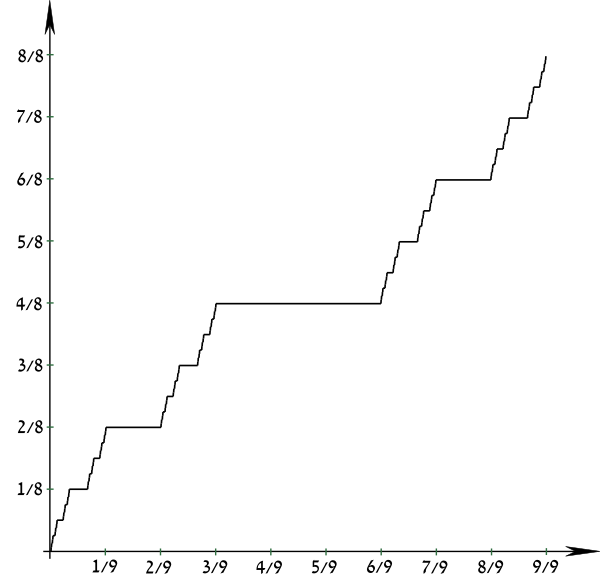
\includegraphics[scale=0.3]{img/devils_staircase.png}
      \caption{Plot} 
      \label{fig:devils_staircase}
    \end{figure}
  \end{definition} 

  \begin{theorem}
    $\phi$ is a nondecreasing, continuous function s.t. $\phi^\prime (x) = 0$ for all $x \in O$ and $m(O) = 1$. 
  \end{theorem}
  \begin{proof}
    Listed. 
    \begin{enumerate}
      \item \textit{Increasing}. $\phi$ is increasing on each $O_k$, and so on $O$. Then, it is also increasing on $C$ by definition. 
      \item \textit{Continuity}. If $x \in C$, it lies between 2 intervals of $O_k$ for any $k$. The difference in function values between 2 neighboring intervals of $O_k$ is $2^{-k}$, so $\phi$ is continuous. 
      \item \textit{Derivative}. The derivative is $0$ because it is constant around an interval. 
    \end{enumerate}
  \end{proof}

  \begin{theorem}[]
    Define $\psi (x) = \phi(x) + x$. Then, 
    \begin{enumerate}
      \item $\psi$ is continuous and strictly increasing. 
      \item $\psi$ maps $C$ into a set of positive measure. 
      \item $\psi$ maps some subset of $C$ into a nonmeasurable set. 
    \end{enumerate}
  \end{theorem}
  \begin{proof}
    Listed. 
    \begin{enumerate}
      \item Continuity is from sum of continuous functions, and strictly increasing since $\phi$ is nondecreasing and $x$ is strictly increasing. 
      \item We know that $\psi([0, 1]) = [0, 2]$ and $m(\psi(O))= 1$, where for each interval $I_j \subset O$, $m(\psi(I_j)) = \ell(I_j)$. Therefore, $m(\psi(C)) = 1$. 
      \item Since $\psi$ is strictly increasing, there exists a continuous inverse $\psi^{-1}$. Find $Z \subset \psi(C)$ that is nonmeasurable, which we can do from the previous theorem. Then, there exists $E \subset C$ s.t. $\psi(E) = Z$, and $E$ is not Borel since if it were, then $Z$ would be Borel, too. 
    \end{enumerate}
  \end{proof}


\section{Measurable Functions}

  So far, we have defined measurable sets, constructed the Lebesgue measure, and shown that Lebesgue measurable sets can be approximated by nice open sets. Now, let's talk about measurable functions. Just like for measurable sets, there is a general sense in which we can define them and there is the more ``Euclidean'' way of defining them. 

  \begin{definition}[Measurable Function]
    Given a measurable space $(X, \mathcal{A})$, $f: (X, \mathcal{A}) \longrightarrow \mathbb{R}$ is \textbf{measurable} if 
    \begin{equation}
      f^{-1}(A) \in \mathcal{A} \text{ for all } A \text{ open}
    \end{equation}
    Note that measurable functions are always defined on measurable sets, so we don't have to state that its domain is always measurable. 
  \end{definition}

  \begin{theorem}[Measurable Functions on Real Line]
    Let $f: E \subset \mathbb{R} \to \mathbb{R} \cup \{ \pm \infty\}$ and $E$ be measurable. Then, TFAE 
    \begin{enumerate} 
      \item $\forall c \in \mathbb{R}$, $\{x \in E \mid f(x) > c\}$ is measurable. 
      \item $\forall c \in \mathbb{R}$, $\{x \in E \mid f(x) \geq c\}$ is measurable. 
      \item $\forall c \in \mathbb{R}$, $\{x \in E \mid f(x) < c\}$ is measurable. 
      \item $\forall c \in \mathbb{R}$, $\{x \in E \mid f(x) \leq c\}$ is measurable. 
      \item $f$ is Lebesgue measurable. 
    \end{enumerate}
    Furthermore, if any of these hold, then also $\{x \in E \mid f(x) = c \}$ is measurable for all $c$ (but not the converse!). 
  \end{theorem} 
  \begin{proof}
    We know that $(1) \iff (4)$ and $(2) \iff (3)$ by taking complements. We prove $(1) \iff (2)$. 
    \begin{enumerate}
      \item $(1) \implies (2)$. 
      \begin{equation}
        \{x \in E \mid f(x) \geq c \} = \bigcap_{k=1}^\infty \{x \in E \mid f(x) > c - \frac{1}{k} \}
      \end{equation}

      \item $(2) \implies (1)$. 
      \begin{equation}
        \{ x \in E \mid f(x) > c\} = \bigcup_{k=1}^\infty \{x \in E \mid f(x) \geq c + \frac{1}{k} \}
      \end{equation}
    \end{enumerate}

    For $(5)$, we know that
    \begin{enumerate}
      \item $(5) \implies (1)$ is trivial, since open intervals are open sets. 
      \item $(1) \implies (5)$. Any open set is a countable union of disjoint open intervals, and so let 
      \begin{equation}
        U = \bigcup_{k=1}^\infty I_k, \qquad I_k = (a_k, b_k) = \underbrace{(-\infty, b_k)}_{B_k} \cap \underbrace{(a_k, +\infty)}_{A_k}
      \end{equation} 
      Therefore, 
      \begin{equation}
        f^{-1} (U) = \bigcup_{k=1}^\infty f^{-1} (B_k \cap A_k) = \bigcup_{k=1}^\infty \{f^{-1} (B_k) \cap f^{-1} (A_k) \}
      \end{equation}
      which is measurable since countable union/intersections are measurable (by definition of $\sigma$-algebra). 
    \end{enumerate}

    For the final implication, we can use $(2)$ and $(4)$ to get 
    \begin{equation}
      \{x \in E \mid f(x) = c\} = \{x \in E \mid f(x) \leq c \} \cup \{x \in E \mid f(x) \geq c \}
    \end{equation}
  \end{proof} 

  The first question is how you would relate this to continuity. 

  \begin{theorem}[Continuous Functions are Measurable]
    If $f: X \to \mathbb{R}$ is continuous, then it is measurable. 
  \end{theorem}
  \begin{proof}
    If $f$ is continuous, then $f^{-1} (O) = U \cap X$ for every open $O$ with open $U$. 
  \end{proof}

  \begin{theorem}[Monotonic Functions are Measurable] 
    Let $I$ be an interval. If $f: I \subset \mathbb{R}$ is monotone, then $f$ is measurable.
  \end{theorem}
  \begin{proof}
    You can probably see that it is more advantageous to prove using the definition of measurability using rays. We wish to show that for all $c$, $E_c \coloneqq \{x \in I \mid f(x) > c\}$ is measurable. We wish to show that $E_c$ is an interval, though there seems to be some complications with potential discontinuities. 

    Therefore, we use an equivalent definition of an interval: $I$ is an interval if for every $x, y \in I$, $x < t < y \implies t \in I$. Therefore, we can see that if $x, y \in E_c$, then $f(x) > c, f(y) > c$. Therefore, if $t$ is in between them, $f(t) > f(\min\{x, y\}) > c$, and so $t \in E_c$. Since intervals are measurable, we are done. 
  \end{proof}

  There is also some notion of robustness. 

  \begin{theorem}[Function Difference on Measure 0 Set Doesn't Affect Measurability]
    Suppose $f: E \subset \mathbb{R} \to \mathbb{R} \cup \{\pm \infty\}$ with $E$ measurable, and let $g$ be some other function. If $f$ is measurable on $E$ and $g(x) = f(x)$ a.e. for $x \in E$, then $g$ is measurable on $E$. 
  \end{theorem}
  \begin{proof}
    We wish to show that for any open $O \subset \mathbb{R}$, $g^{-1} (O)$ is measurable. We might start with Carathéodory and try to show that for all $A \subset E$, 
    \begin{equation}
      m^\ast(A) = m^\ast (A \cap g^{-1}(O)) + m^\ast (A \cap g^{-1}(O)^c)
    \end{equation}
    But this turns out to be overkill. Since this is about $0$ measure sets, you should be thinking about how $0$-measure sets do not affect measurability and try to use this. In $g^{-1}(O)$, there is a portion of it that overlaps with $f$---call it $A \subset E$---and a portion that doesn't. We know that $m^\ast (E \setminus A) = 0$\footnote{TBD: Can we write $m$? } and a measure $0$ set difference doesn't affect measurability, so $A$ is measurable. So let's decompose it. 
    \begin{align}
      g^{-1} (O) & = \big( g^{-1} (O) \cap A \big) \cup \big( g^{-1} (O) \cap (E \setminus A) \big) \\ 
                 & = \big( f^{-1} (O) \cap A \big) \cup \big( g^{-1} (O) \cap (E \setminus A) \big)
    \end{align}
    If we try to take the measure of this, the first term is the union of measurable sets $f^{-1} (O)$ and $A$. The second term is also measurable since the outer measure is $0$, by subadditivity compared to $m^\ast(E \setminus A) = 0$. Therefore $g^{-1} (O)$ is measurable. 
  \end{proof}
  \begin{proof}
    In class. Consider $S = \{x \in E \mid g(x) < c \}$. Let $A \subset E$ be the set where $g(x) = f(x)$, with $m (E \setminus A) = 0$. Then, 
    \begin{equation}
      S = \big( \{x \in E \mid g(x) < c\} \cap (E \setminus A) \big) \cup \big( \{x \in E \mid f(x) < c\} \cap A \big) 
    \end{equation}
    where the first term is measure $0$ by monotonicity with $E \setminus A$, $m(E \setminus A) = 0$, and the second term is measurable since $A = E \setminus (E \setminus A)$. So, $S$ is measurable. 
  \end{proof}

  You preserve measurability if you split the domain in a ``measurable way.'' 

  \begin{theorem}[Measurable Partition Induces Measurable Restrictions of Functions]
    Take a measurable subset $D \subset E$ and let $f: E \to \mathbb{R} \cup \{\pm\infty\}$ be a function. Then, the following are equivalent. 
    \begin{enumerate}
      \item $f$ is measurable on $E$ 
      \item $f$ is measurable on $D$ and on $E \setminus D$. 
    \end{enumerate}
  \end{theorem}
  \begin{proof}
    We prove bidirectionally. 
    \begin{enumerate}
      \item $(\rightarrow)$. Let's prove measurability on $D$. We can see that 
      \begin{equation}
        \{x \in D \mid f(x) \in O \} = \{x \in E \mid f(x) \in O \} \cap D
      \end{equation}
      as the intersection of measurable sets, is measurable. Then we can just take the complement of both sides to get. 
      \begin{align}
        \{x \in E \setminus D \mid f(x) \in O\} 
          & = E \setminus \{x \in D \mid f(x) \in O \} \\ 
          & = E \setminus \big( \{x \in E \mid f(x) \in O \} \cap D \big) \\
          & = \underbrace{\big( E \setminus \{x \in E \mid f(x) \in O \} \big)}_{\text{measurable}} \cup \underbrace{\big( E \setminus D \big)}_{\text{measurable}}
      \end{align}
      which is also measurable. 

      \item $(\leftarrow)$. Take some open $O \subset \mathbb{R} \cup \{\pm\infty\}$ and take its preimage. Then, 
      \begin{equation}
        f^{-1} (O) = \{x \in D \mid f(x) \in O\} \cup \{x \in E \setminus D \mid f(x) \in O \}
      \end{equation} 
      as the finite union and intersection of measurable sets, is measurable. 
    \end{enumerate}
  \end{proof}

\subsection{Arithmetic and Composition of Measurable Functions}

  The following theorem is useful, since we don't want to manually check measurability of every single new function we create. 

  \begin{theorem}[Arithmetic on Measurable Functions]
    Given measurable functions $f, g: E \subset \mathbb{R} \to \mathbb{R}$, the following standard operations on them create new measurable functions: 
    \begin{enumerate}
      \item $\alpha f$ is measurable for all $\alpha \in \mathbb{R}$. 
      \item $f + g$ is measurable 
      \item $f \cdot g$ is measurable 
      \item $f / g$ is measurable on $\{x \mid g(x) \neq 0\}$ 
    \end{enumerate}
  \end{theorem} 
  \begin{proof}
    WLOG, we can assume $f, g$ are finite everywhere since changing these values to finite values over a set of measure $0$ doesn't affect measurability. 
    \begin{enumerate}
      \item If $\alpha = 0$, this is trivially true. If not, then 
      \begin{equation}
        \{ x \in E \mid (\alpha f) (x) < c \} = \{x \in E \mid f(x) < \frac{c}{\alpha} \} 
      \end{equation}

      \item Suppose $f(x) + g(x) < c \iff f(x) < c - g(x) \iff \exists q \in \mathbb{Q}$ s.t. $f(x) < q < c - g(x)$.\footnote{The reason we want to introduce rationals is that we want to take advantage of countability.} Then, 
      \begin{equation}
        \{x \in E \mid f(x) + g(x) < c \} = \bigcup_{q \in \mathbb{Q}} \big( \{x \in E \mid f(x) < q\} \cap \{x \in E \mid g(x) < c - q \}\big)
      \end{equation}
      which is a countable union of measurable sets, and is measurable. 

      \item We use a nice trick from analysis. 
      \begin{equation}
        fg = \frac{1}{4} \big( (f + g)^2 - (f - g)^2 \big) 
      \end{equation}
      and so it suffices to prove that $h$ measurable implies $h^2$ measurable. For $c \geq 0$\footnote{We only need to consider this case since $h^2$ is always nonnegative and so $c < 0$ would mean preimage is empty set.}, we have 
      \begin{equation}
        \{ x \in E \mid h^2 (x) > c \} = \{x \in E \mid h(x) > \sqrt{c} \} \cup \{x \in E \mid h(x) < -\sqrt{c} \}
      \end{equation}

      \item 
    \end{enumerate}
  \end{proof}

  \begin{theorem}[Finite Min/Max of Measurable Functions are Measurable]
    If $f_1, \ldots, f_n: E \subset \mathbb{R} \to \mathbb{R}$ are measurable, then so are $\max_k f_k$ and $\min_k f_k$. 
  \end{theorem}
  \begin{proof}
    We can prove by induction, but this is still a one-liner. For maximum, 
    \begin{equation}
      \{x \in E \mid (\max_k{f_k})(x) > c \} = \bigcup_{k=1}^n \{x \in E \mid f_k (x) > c\} 
    \end{equation}
    and for the minimum, 
    \begin{equation}
      \{x \in E \mid (\min_k{f_k})(x) > c \} = \bigcap_{k=1}^n \{x \in E \mid f_k (x) > c\} 
    \end{equation}
  \end{proof} 

  \begin{example}[Composition of Two Functions need not be Measurable]
    Recall from \ref{thm:pathological-devils-staircase} that we built a function $\psi(x)$ that maps some measurable $A$ to nonmeasurable $\psi(A)$. Let's extend $\psi$ to all $\mathbb{R}$ and keep it strictly increasing. Let $\chi_A$ be the characteristic function of $A$. Consider $f = \chi_A \circ \psi^{-1}$, and take the preimage of $(1/2, +\infty)$ under $\psi$. 
    \begin{equation}
      f^{-1} ((\frac{1}{2}, +\infty)) = \{x \mid \psi^{-1} (x) \in A \}  = \{x \in \psi(A)\} = \psi(A)
    \end{equation}
    which we have proven  that there exists some $A$ s.t. $\psi(A)$ is not measurable. 
  \end{example}

  So this is bad news, but we have a compromise. 

  \begin{theorem}[Composition of Measurable then Continuous is Measurable]
    Suppose $g$ is measurable on $E$, $f$ is continuous on $\mathbb{R}$. Then, $f \circ g$ is measurable. 
  \end{theorem}
  \begin{proof}
    Take any open $O$. Then, 
    \begin{equation}
      (f \circ g)^{-1} (O) \iff g(x) \in f^{-1} (O) 
    \end{equation}
    where $f^{-1} (O)$ is open, which implies measurable. 
  \end{proof}

  So we get much more results, like that $|f|$ or $|f|^p$ is measurable if $f$ is measurable. 

\subsection{Sequences of Measurable Functions}

  Let's compare continuous functions and measurable functions. In terms of composition, continuity is a little more robust since we can compose continuous functions to get continuous functions. Meanwhile, we know that measurable functions don't necessarily compose to measurable functions. The relation is reversed when we talk about convergence. Recall from analysis the definitions of \hyperref[real-def:pointwise-convergence]{pointwise convergence} and \hyperref[real-def:uniform-convergence]{uniform convergence} of a sequence of functions. First, we present an analogous measure-theoretic definition of pointwise convergence. 

  \begin{definition}[Almost Sure Convergence]
    A sequence of functions $(f_n: E \to \mathbb{R})_n$ is said to \textbf{converge almost surely to $f$} if $f_n (x) \to f(x)$ for all $x \in A \subset E$ where $m(E \setminus A) = 0$. 
  \end{definition}

  If you have uniform convergence, this is great since the uniform limit of continuous (Riemann integrable) functions is continuous (Riemann integrable). However, the pointwise limit of continuous (Riemann integrable) functions may fail to be continuous (Riemann integrable). It turns out that measurability is preserved through almost sure convergence. 

  \begin{theorem}[Almost Sure Convergence of Measurable Functions are Measurable]
    Suppose $f_n$ are measurable on $E$ and $f_n \to f$ a.e. on $E$. Then, $f$ is measurable. 
  \end{theorem}
  \begin{proof}
    WLOG, $f_n \to f$ at all $x \in E$ (since behavior on measure $0$ sets don't affect measurability). Now, consider $\{x \in E \mid f(x) < c\}$. Then, $f(x) < c \iff \exists n, N \in \mathbb{N}$ s.t. $f_k (x) < c - \frac{1}{n}$ for all $k \geq N$. Observe that $\{x \in E \mid f_k (x) < c - \frac{1}{n}\}$ is measurable, so 
    \begin{equation}
      \int_{k = N}^\infty \{ x \in E \mid f_k (x) < c - \frac{1}{n} \}
    \end{equation}
    is also measurable. But 
    \begin{equation}
      \{ x \in E \mid f(x) < c\} = \bigcup_{n, N = 1}^\infty \bigg( \bigcap_{k=N}^\infty \{ x \in E \mid f_k (x) < c - \frac{1}{n} \} \bigg) 
    \end{equation}
    is again also measurable. 
  \end{proof}

  So though continuous functions are more robust w.r.t. composition, measurable functions are more robust w.r.t. convergence. 

\subsection{Nearly Uniform Convergence of Measurable Functions} 

  This is one of the major ideas in measure theory. 

  \begin{lemma} 
    Let $(f_n: E \subset \mathbb{R} \to \mathbb{R})$ be a sequence of measurable functions with $m(E) < +\infty$ that converges pointwise to $f$. Then, for each $\eta > 0$ and $\delta > 0$, there exists a measurable subset $A \subset E$ and index $N$ such that 
    \begin{equation}
      |f_n - f| < \eta \text{ on } A \text{ for all } n \geq N, \text{ and } m(E \setminus A) < \delta 
    \end{equation}
  \end{lemma}
  \begin{proof}
    
  \end{proof}

  The next theorem is one we will use all the time. It basically tells us a way to turn a sequence of pointwise convergent functions into a sequence of uniformly convergent functions. It seems similar to \hyperref[real-thm:dini]{Dini's theorem}. 

  \begin{theorem}[Egorov]
    Let $(f_n: E \subset \mathbb{R} \to \mathbb{R})$ be a sequence of measurable functions with $m(E) < +\infty$ that converges pointwise to $f$. Then, for each $\epsilon > 0$, there exists a closed set $F \subset E$  s.t. 
    \begin{equation}
      f_n \to f \text{ uniformly on } F \text{ and } m(E \setminus F) < \epsilon
    \end{equation}
  \end{theorem}
  \begin{proof}
    
  \end{proof}

\subsection{Continuous Approximations of Measurable Functions}

  So if we throw out a small set, we can approximate measurable functions with continuous functions. Consider a generalization of step functions called \textit{simple functions}. 

  \begin{definition}[Simple Functions]
    For $A \subset X$ (any subset, not just in some $\sigma$-algebra), the \textbf{characteristic}, or \textbf{indicator} \textbf{function} of $A$ is the function $\chi_A : X \longrightarrow \mathbb{R}$ defined 
    \begin{equation}
      \chi_A (x) = \begin{cases} 1 & \text{ if } x \in A \\ 0 & \text{ if else} \end{cases}
    \end{equation}
    A function $\phi: \mathbb{R} \longrightarrow \mathbb{R}$ is called a \textbf{simple function} if it is a finite linear combination of characteristic functions. 
    \begin{equation}
      \phi = \sum_{i=1}^n a_i \chi_{A_i}
    \end{equation}
  \end{definition} 

  \begin{lemma}[Luzin, for Simple Functions]
    Suppose $f: E \subset \mathbb{R} \to \mathbb{R}$ is simple. Then $\forall \epsilon > 0$, $\exists$ a closed $F \subset E$, $g \in C(\mathbb{R})$, s.t. $f|_F = g |_F$ and $m(E \setminus F) < \epsilon$. 
  \end{lemma}
  \begin{proof}
    
  \end{proof}

  \begin{theorem}[Luzin]
    Suppose $f: E \subset \mathbb{R} \to \mathbb{R}$ is measurable. Then $\forall \epsilon > 0$, $\exists$ a closed $F \subset E$, $g \in C(\mathbb{R})$, s.t. $f|_F = g |_F$ and $m(E \setminus F) < \epsilon$. 
  \end{theorem}
  \begin{proof}
    Assume $m(E) < \infty$. If it is $\infty$, then we can divide the set into countable sets, each with finite measure, and we can do it for $\epsilon/2^{n}$. So it suffices for finite measure. Suppose $f_n$ are simple and $f_n \to f$ pointwise on $E$. By the lemma, we can find closed $F_n \subset E$ s.t. $m(E \setminus F_n) < \epsilon / 2^{n+1}$ and $g_n \in C(\mathbb{R})$, with $g_n |_{F_n} = f_n |_{F_n}$. Also, by Egorov, we can find $F_0$ s.t. $f_n$ converges uniformly on $F_0$, and $m(E \setminus F_0) < \epsilon / 2$. Define 
    \begin{equation}
      F = \bigcap_{n=0}^\infty F_n, \qquad E \setminus F = \bigcup_{n=0}^\infty E \setminus F_n
    \end{equation}
    Then by subadditivity,
    \begin{equation}
      m(E \setminus F) \leq \sum_{n=0}^\infty m(E \setminus F_n) < \epsilon
    \end{equation}
    Finally, $f_n$ converges uniformly on $F$ and $f_n |_F = g_n |_F$, so $f_n$ are continuous on $F$. Since uniform limit of continuous functions is continuous, the limit $f$ is continuous on $F$. 
  \end{proof}

  This is an argument for the interval, but this can be generalized to more general sets. 

\subsection{Simple Approximations of Measurable Functions}

  \begin{lemma}[Simple Approximations Lemma]
    Assume $f$ is bounded on $E \subset \mathbb{R}$, measurable. For every $\epsilon > 0$, there exists simple functions $\phi_\epsilon, \psi_\epsilon$ s.t. 
    \begin{equation}
      \phi_\epsilon \leq f \leq \psi_\epsilon, \qquad \psi_\epsilon - \phi_\epsilon \leq \epsilon
    \end{equation}
    for all $x \in E$. 
  \end{lemma}
  \begin{proof}
    Suppose $|f(x)| \leq M$. Consider a ``partition of $[-M, M]$ into intervals of size $\epsilon$. 
    \begin{equation}
      y_0 = -M < y_1 < y_2 < \ldots < y_{n-1} < y_n = M
    \end{equation}
    where $y_k - y_{k-1} = h < \epsilon$ for all $k$. Define $E_k = f^{-1} ([y_{k-1}, y_k])$, which are measurable. Then, we define 
    \begin{equation}
      \phi_\epsilon(x) = \sum_{k=1}^n y_{k-1} \chi_{E_k} (x) , \qquad \psi_\epsilon (x) = \sum_{k=1}^n y_k \chi_{E_k} (x) 
    \end{equation}
    and can show that this satisfies the properties. 
  \end{proof}

  \begin{theorem}[Simple Approximation Theorem]
    Let $f: E \subset \mathbb{R} \cup \{ \pm \infty\}$ be measurable. Then, there is a sequence of simple functions $\phi_n$ s.t. $\phi_n \to f$ for all $x \in E$, and $\| \phi_n (x) \| \leq \| f(x) \|$ for all $x \in E$. 
  \end{theorem}
  \begin{proof}
    We give a general picture of this proof for a function $f: \mathbb{R} \longrightarrow [0, \infty]$. We can first divide the codomain of the graph below into segments of $t = 1, 2, \ldots$, and take the preimage of all these units under $f$ to get $f_1$. More specifically, $A_1^t = f^{-1} ([t, \infty])$ for all $t$. By measurability of $f$, $A_1^t$ is measurable, and we can assign $f_1 = \chi_{A^1_1} + \chi_{A_1^2} \leq f$. 
    \begin{center}
      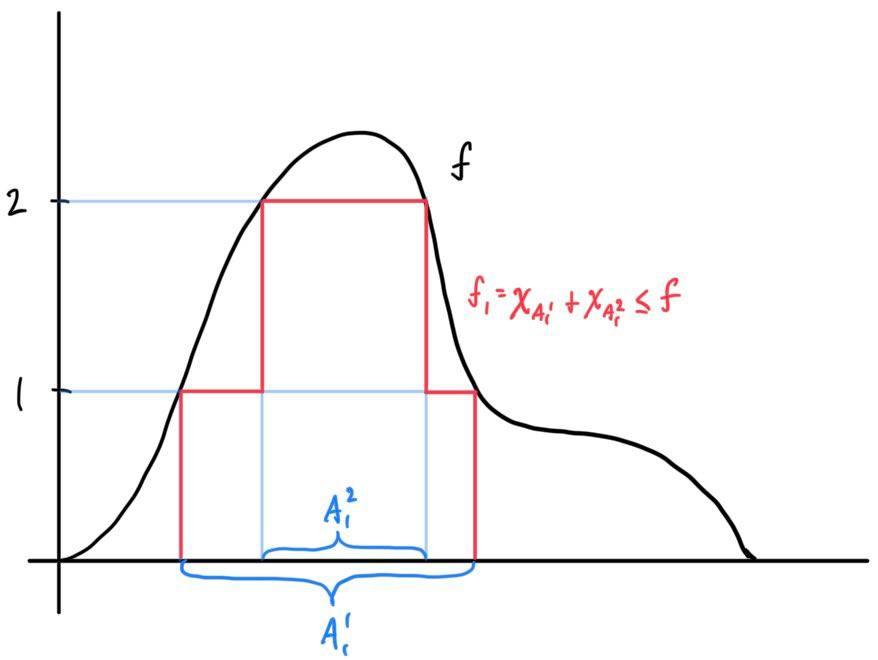
\includegraphics[scale=0.23]{img/Lebesgue_1.jpg}
    \end{center}
    Doing this again with finer subintervals of the codomain gives us, with $f_2 = \chi_{A_2^1} + \chi_{A_2^2} + \chi_{A_2^3} + \chi_{A_2^4} \leq f$. 
    \begin{center}
      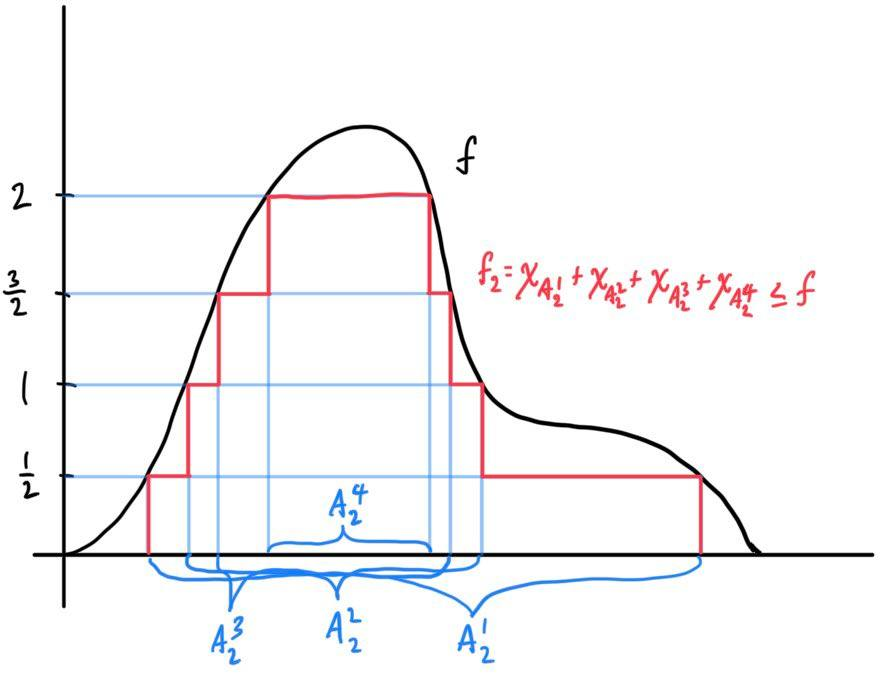
\includegraphics[scale=0.23]{img/Lebesgue_2.jpg}
    \end{center}
    and in general, we have $f_k = \sum_{j=1}^\infty \frac{1}{2^{k-1}} \chi_{A^j_k}$. But we said a simple function is a \textit{finite} sum, and if $\infty$ is in the range of $f$, then this becomes a problem. We can quickly fix this by just truncating the summation at a certain point in the codomain ($f_1$ only considers intervals up to $1$, $f_2$ up to $2$ and so on), ultimately giving us 
    \begin{equation}
      f_k = \sum_{j=1}^{k 2^{k-1}} \frac{1}{2^{k-1}} \chi_{A^j_k} 
    \end{equation}
  \end{proof}


\section{Integration}

  \subsection{Construction of the Riemann Integral}

    We shall first define the integral using the familiar notation of Riemann sums. 

    \begin{definition}[Partitions with Distinguished Points]
      A \textbf{partition} $P$ of a closed interval $[a, b]$, $a < b$, is a finite system of points $x_0, \ldots, x_n$ of the interval such that
      \[a = x_0 < x_1 < x_2 < \ldots < x_n = b\]
      The intervals $[x_{i-1}, x_i]$, $i = 1, 2, \ldots, n$, are called the \textbf{intervals} of the partition $P$. The largest of the lengths of the intervals of the partition $P$, denoted $\lambda(P)$, is called the \textbf{mesh} of the partition. 

      A \textbf{partition with distinguished points} $(P, \xi)$ on the closed interval $[a, b]$ is a partition $P$ of $[a,b]$ along with the set of $n$ points 
      \[\xi_1 \in [x_0, x_1], \xi_2 \in [x_1, x_2], \ldots, \xi_n \in [x_{n-1}, x_n]\]
      The $n$-tuple of $\xi_i$'s is denoted by the single letter $\xi$
      \[\xi = (\xi_1, \xi_2, \ldots, \xi_n)\]
    \end{definition}

    This naturally leads to the following construction. 

    \begin{definition}[Riemann Sums]
      If a function $f$ is defined on a closed interval $[a, b]$ and $(P, \xi)$ is a partition with distinguished points on this closed interval, the sum
      \[\sigma(f; P, \xi) \equiv \sum_{i=1}^n f(\xi_i)\, \Delta x_i, \text{ where } \Delta x_i = x_i - x_{i-1},\]
      is the \textbf{Riemann sum} of the function $f$ corresponding to the partition $(P, \xi)$ with distinguished points on $[a, b]$. 
      \begin{center}
          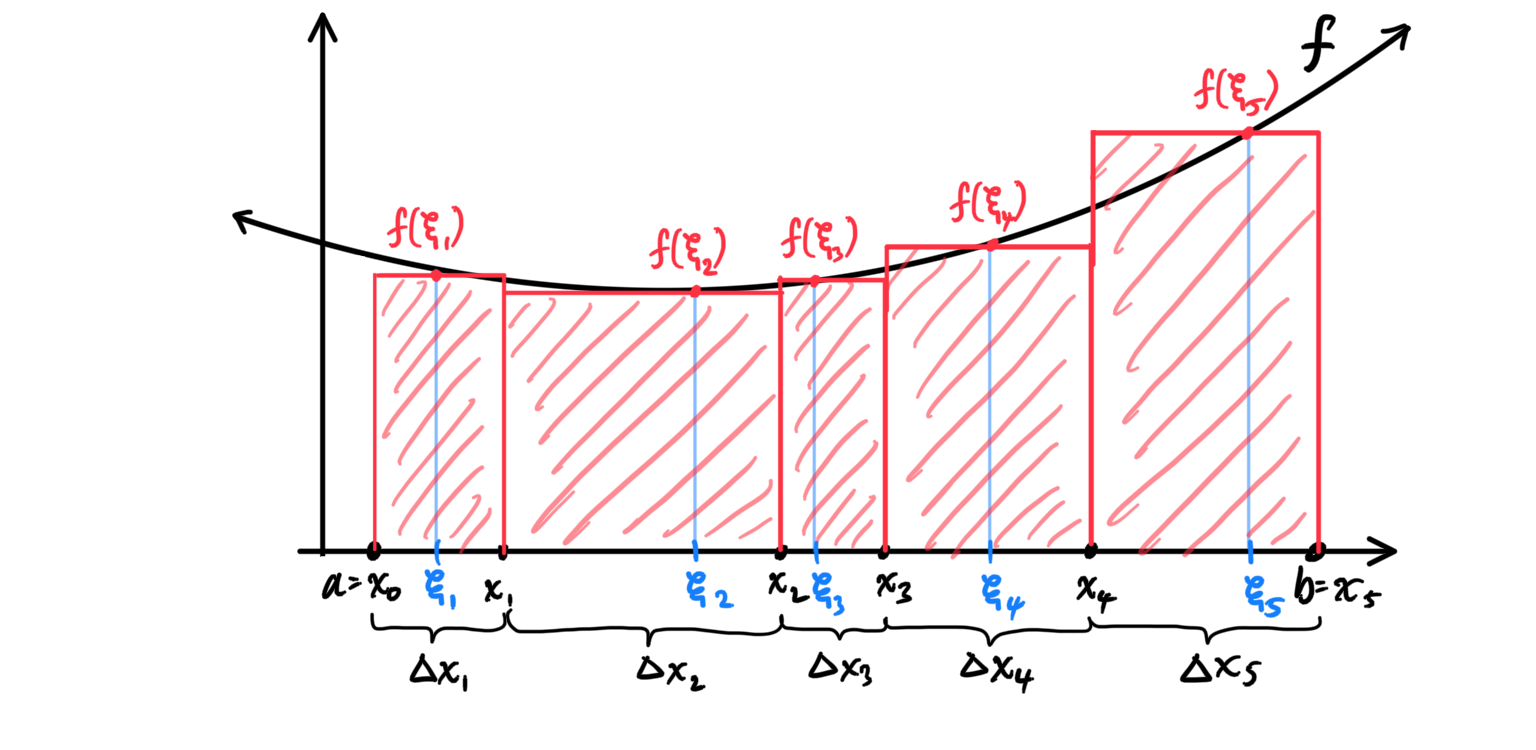
\includegraphics[scale=0.25]{img/Riemann_Sum_with_Partitions_Points.PNG}
      \end{center}
      Thus, when a function $f$ is fixed, the Riemann sum $\sigma (f; P, \xi)$ is a mapping that takes in a partition with distinguished points $p = (P, \xi)$ on the closed interval $[a, b]$ and outputs a number representing the total area of the Riemann sums. That is, for a fixed $f$ and some input $p = (P, \xi)$, we can define the function 
      \[\Phi: \mathcal{P} \longrightarrow \mathbb{R}, \;\;\; \Phi(p) \equiv \sigma(f; p) \equiv \sigma(f; (P, \xi))\]
      that takes in a partition with distinguished points on $[a,b]$ and outputs the corresponding Riemann sum for that fixed $f$. 
    \end{definition}

    \begin{definition}[Riemann Integral]
      The number $\int_a^b f(x)\,dx$ is the \textbf{Riemann integral} of the function $f$ on the closed interval $[a, b]$ if for every $\epsilon>0$ there exists a $\delta>0$ such that
      \[\Bigg| \int_a^b f(x)\,dx - \sum_{i=1}^n f(\xi_i) \Delta x_i \Bigg| < \epsilon\]
      for any partition $(P, \xi)$ with distinguished points on $[a, b]$ whose mesh $\lambda(P)$ is less than $\delta$. We can view this as a limit where $n \rightarrow \infty$, but there is a problem since we can increase the partition within different subsets of $[a,b]$, leading to multiple values of convergence. 
      \begin{center}
          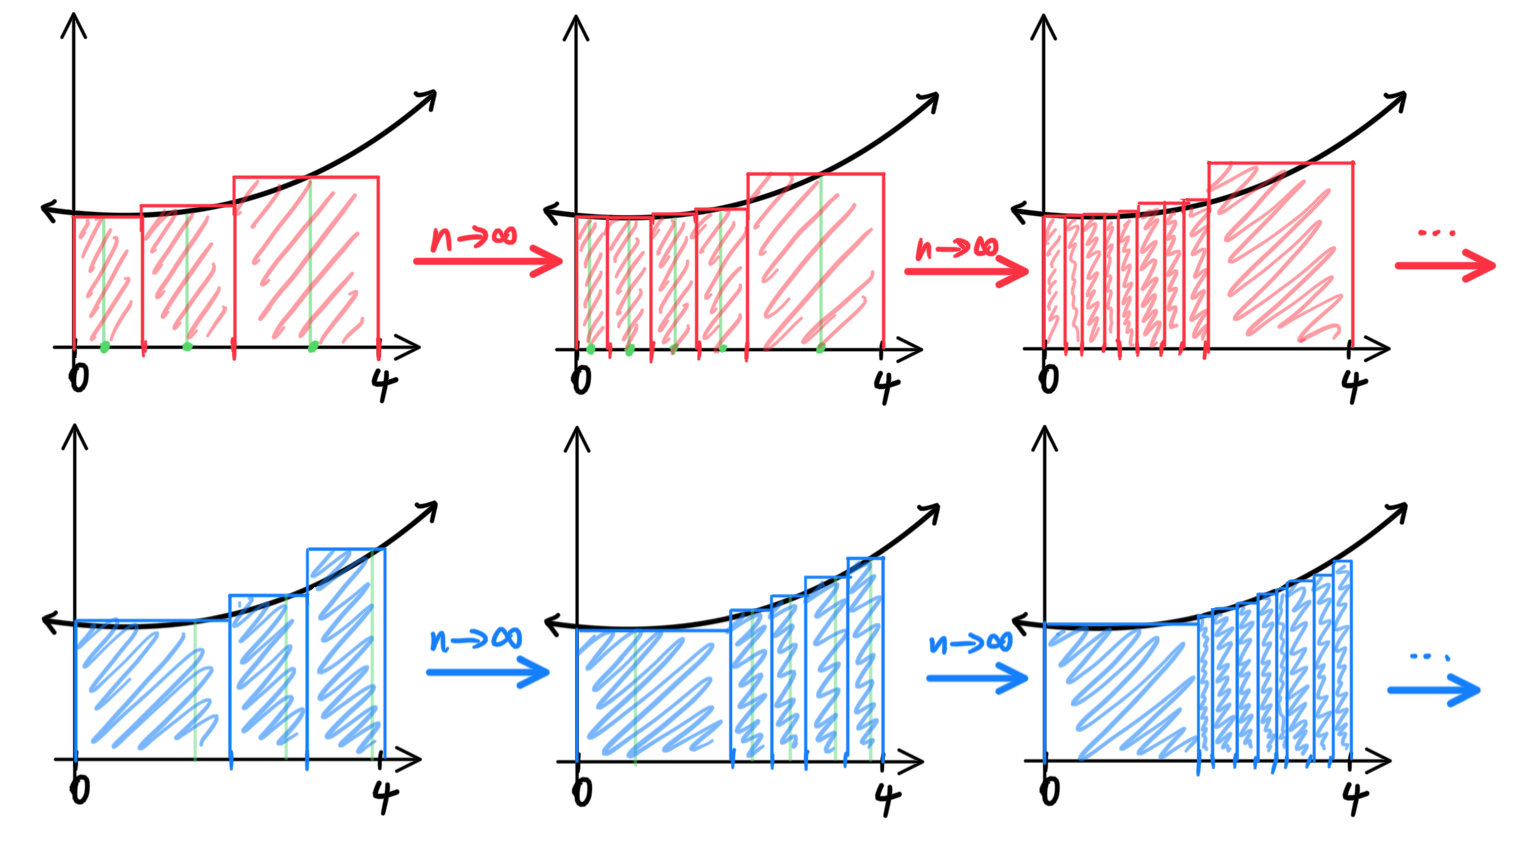
\includegraphics[scale=0.28]{img/Riemann_Integral_Converging_onto_2_Numbers.PNG}
      \end{center}
      Rather, we can set the mesh $\lambda(P)$ to approach $0$, which would take care of the problems. We can visualize this by imagining the lengths of the rectangles converging "uniformly."
      \begin{center}
          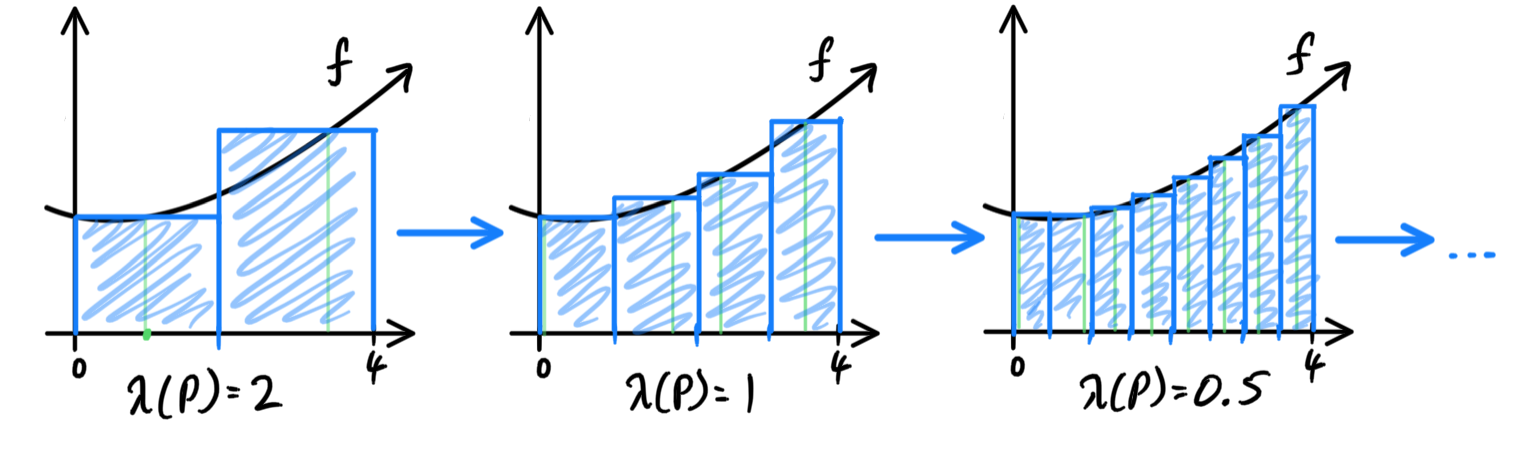
\includegraphics[scale=0.28]{img/Riemann_Integral_Limit_Mesh_goes_to_0.PNG}
      \end{center}
      Therefore, we can culminate by defining the Riemann integral of $f(x)$ over $[a,b]$ as 
      \[\int_a^b f(x)\,dx \equiv \lim_{\lambda(P) \rightarrow 0} \sum_{i=1}^n f(\xi_i) \lambda x_i\]
    \end{definition}

  \subsubsection{Conditions for Integrability}

    \begin{definition}[Riemann Integrable Functions]
      A function $f$ is \textbf{Riemann integrable} on the closed interval $[a, b]$ if 
      \[\int_a^b f(x)\,dx \equiv \lim_{\lambda(P) \rightarrow 0} \sum_{i=1}^n f(\xi_i) \lambda x_i\]
      is defined, i.e. if the limit of the right-hand side of Riemann sums exists as $\lambda(P) \rightarrow 0$ (that is, the Riemann integral of $f$ is defined). 

      Furthermore, the set of Riemann-integrable functions on a closed interval $[a, b]$ is denoted $\mathcal{R}[a,b]$. 
    \end{definition}

    Remember that the Riemann integral, as complicated as the formula is, is still a limit of a function. That means that we can apply the Cauchy criterion to it to determine convergence. 

    \begin{lemma}[Cauchy Criterion on Existence of Riemann Integral]
      Given a function $f$, the integral of $f$ over $[a, b]$, defined
      \[\int_a^b f(x)\,dx \equiv \lim_{\lambda(P) \rightarrow 0} \sum_{i=1}^n f(\xi_i) \lambda x_i\]
      exists if and only if for every $\epsilon>0$, there exists a $\delta>0$ such that 
      \[\big| \sigma(f; P^\prime, \xi^\prime) - \sigma(f; P^{\prime\prime}, \xi^{\prime\prime} \big| < \epsilon\]
      or, what is the same, 
      \[\Bigg| \sum_{i=1}^{n^\prime} f(\xi_i^\prime) \Delta x_i^\prime - \sum_{i=1}^{n^{\prime\prime}} f^(\xi_i^{\prime\prime}) \Delta x_i^{\prime\prime} \Bigg| < \epsilon\]
      for any partitions $(P^\prime, \xi^\prime)$ and $(P^{\prime\prime}, \xi^{\prime\prime})$ with distinguished points on the interval $[a, b]$ with
      \[\lambda(P^\prime), \lambda(P^{\prime\prime}) < \delta\]
      In words, this means that for any $\epsilon>0$ that we choose, there always exists a $\delta>0$ such that \textbf{any} two Riemann sums with mesh size \textbf{both} smaller than $\delta$ will have an error difference of less than $\epsilon$. \begin{center}
          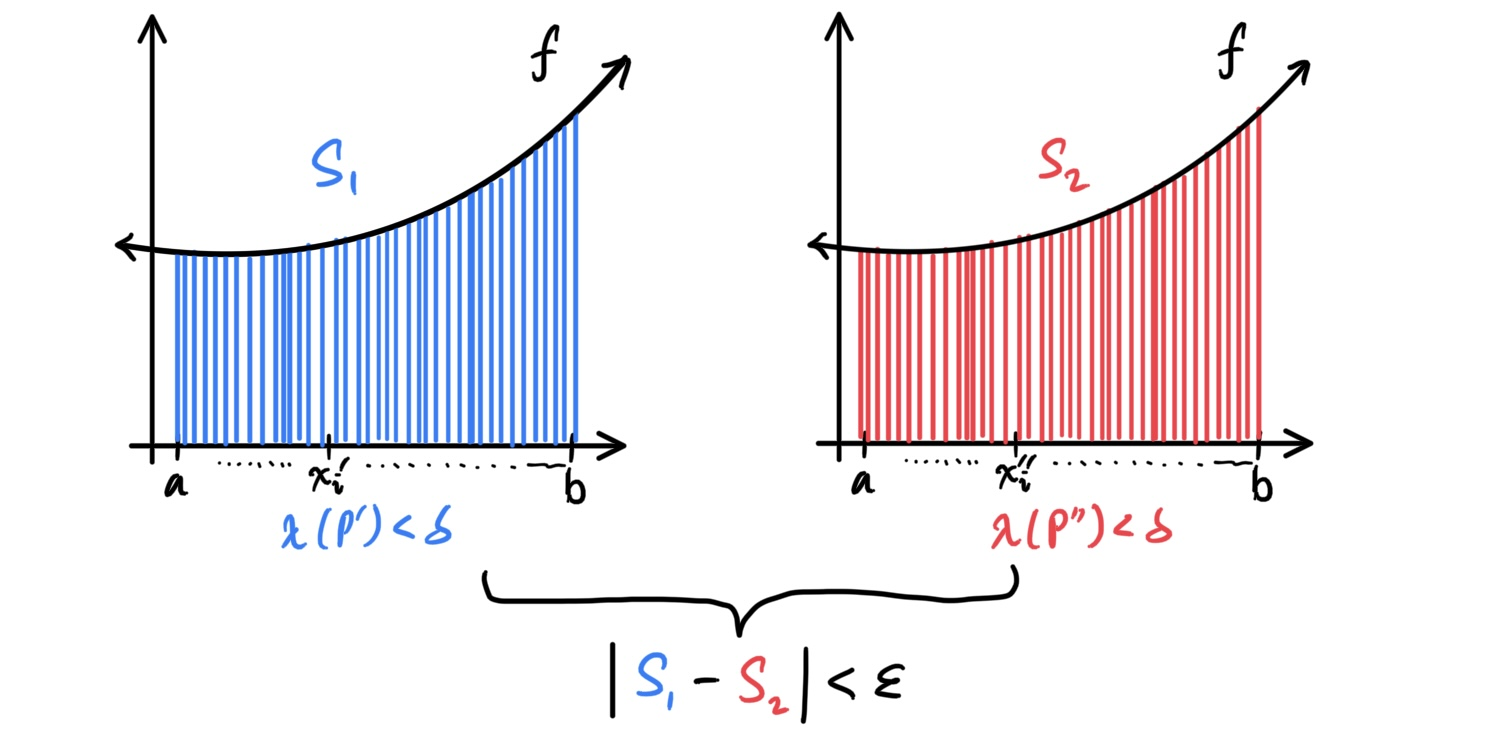
\includegraphics[scale=0.25]{img/Cauchy_Criterion_of_Riemann_Integral.jpg}
      \end{center}
    \end{lemma}

    \begin{theorem}[Necessary Condition for Integrability]
    A necessary condition for $f$ defined on a closed interval $[a, b]$ to be Riemann integrable on $[a, b]$ is that $f$ be bounded on $[a, b]$. That is, 
    \[f \in \mathcal{R}[a, b] \implies f \text{ is bounded on } [a, b]\]
    We can clearly see the necessity of $f$ being bounded by looking at the contrapositive of the following statement. 
    \end{theorem}

    \begin{theorem}[Refinement]
    Given a partition $P$ on interval $[a, b]$, recall that we have points $x_0, \ldots, x_n$ such that
    \[a = x_0 < x_1 < \ldots < x_n = b\]
    Here we introduce new notation: 
    \begin{enumerate}
      \item $\Delta_i$ denotes the interval $[x_{i-1}, x_i]$
      \item $\Delta x_i$ denotes the difference $x_i - x_{i-1}$, i.e. the length of $\Delta_i$
    \end{enumerate}
    If a partition $\Tilde{P}$ of the closed interval $[a, b]$ is obtained from the partition $P$ by the addition of new points to $P$, we call $\Tilde{P}$ a \textbf{refinement} of $P$. 

    When a refinement $\Tilde{P}$ of a partition $P$ is constructed, some (perhaps all) of the closed intervals $\Delta_i = [x_{i-1}, x_i]$ of the partition $P$ themselves undergo partitioning. 
    \[x_{i-1} = x_{i0} < x_{i1} < \ldots < x_{in_i} = x_i\]
    In that connection, it will be useful to label to points of $\Tilde{P}$ by double indices, where in the notation $x_{ij}$ the first index $i$ means that 
    \[x_{ij} \in \Delta_i = [x_{i-1}, x_i]\]
    and the second index $j$ is the ordinal number of the point on the closed interval $\Delta_i = [x_{i-1}, x_i]$. Therefore, it is natural to set the notations
    \begin{enumerate}
      \item $\Delta_{ij} = [x_{i j-1}, x_{ij}]$
      \item $\Delta x_{ij} = x_{ij} - x_{ij-1}$
    \end{enumerate}
    This means that 
    \[\Delta x_i = \Delta x_{i1} + \Delta x_{i2} + \ldots + \Delta x_{in_i}\]
    which can be visualized below
    \begin{center}
      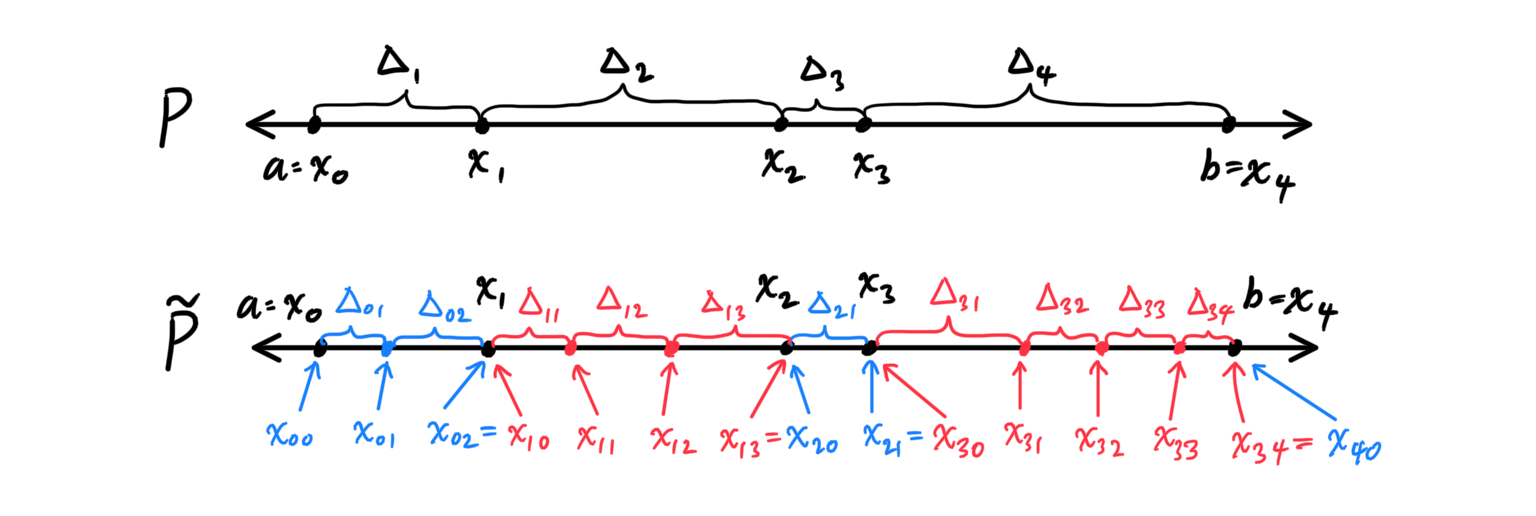
\includegraphics[scale=0.25]{img/Refinement_Definition_Analysis.PNG}
    \end{center}
    \end{theorem}

    \begin{example}[Union of Partitions as a Refinement]
    For some interval $[a, b]$, given partitions $P^\prime$ ($a = x_0 < \ldots < x_n = b$) and $P^{\prime\prime}$ ($a = y_0 < \ldots < y_n = b$), the union of the two partitions $\Tilde{P} = P^\prime \cup P^{\prime\prime}$ is a refinement of both $P^\prime$ and $P^{\prime\prime}$. 
    \begin{center}
        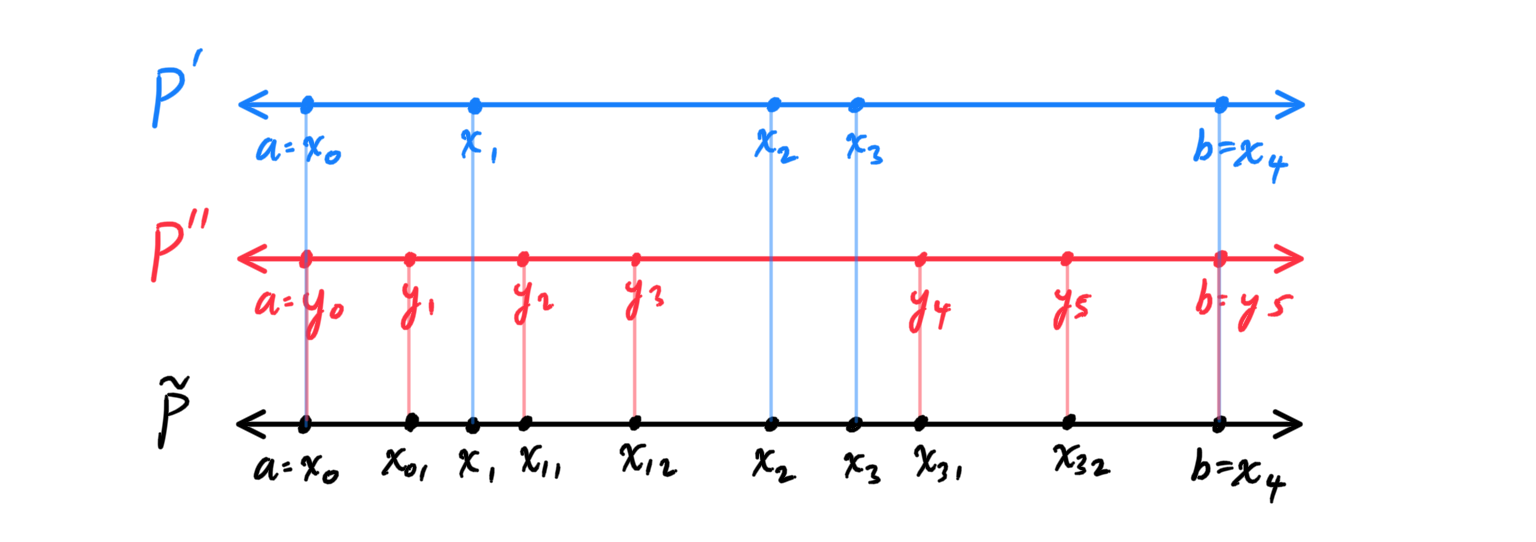
\includegraphics[scale=0.25]{img/Refinement_as_Union_of_Partitions.PNG}
    \end{center}
    \end{example}
    
    Recall that $\omega(f; E)$ denotes the oscillation of the function $f$ on the set $E$; that is, 
    \[\omega(f; E) \equiv \sup_{x^\prime, x^{\prime\prime} \in E} \big| f(x^\prime) - f(x^{\prime\prime})\big|\]
    In particular, $\omega(f; \Delta_i)$ is the oscillation of $f$ on the closed interval $\Delta_i$. 

    \begin{theorem}[Sufficient Condition for Integrability]
    Let $f$ be a bounded on a closed interval $[a, b]$ such that for every $\epsilon > 0$ there exists a number $\delta>0$ such that
    \[\sum_{i=1}^n \omega(f; \Delta_i) \Delta x_i < \epsilon\]
    for any partition $P$ of $[a, b]$ with mesh $\lambda(P) < \delta$. This is equivalent to saying that
    \[\lim_{\lambda(P) \rightarrow 0} \sum_{i = 1}^n \omega (f; \Delta_i) \, \Delta x_i = 0\]
    Then, $f$ is integrable. We can visualize
    \[\sum_{i=1}^n \omega(f; \Delta_i) \Delta x_i\]
    as the following sum of rectangles below. 
    \begin{center}
        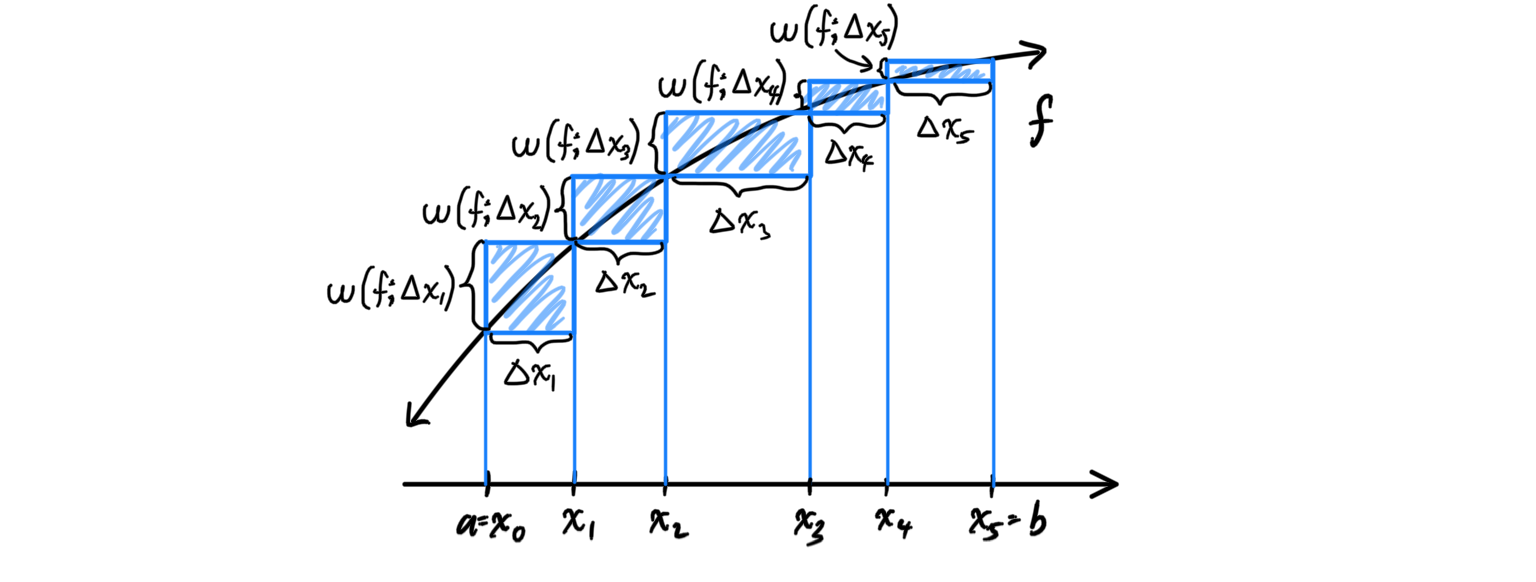
\includegraphics[scale=0.25]{img/Sufficient_Condition_for_Integrability.PNG}
    \end{center}
    What the theorem states, visually, is that as we make all the rectangles smaller and smaller (by putting a limit on the mesh $\lambda(P)<\delta$), we can make the sum of all these rectangles also arbitrarily small. 
    \end{theorem}

    \begin{corollary}[Integrability of Continuous Functions]
    Every continuous function on a closed interval is integrable on that closed interval. That is, 
    \[f \in C[a, b] \implies f \in \mathcal{R}[a, b]\]
    \end{corollary}

    We can actually make a stronger claim. 

    \begin{corollary}[Integrability of Discontinuous Functions]
    If a bounded function $f$ on a closed interval $[a, b]$ is continuous everywhere except at a finite set of points, then $f \in \mathcal{R}[a, b]$. 
    \end{corollary}

    \begin{corollary}[Integrability of Monotonic Functions]
    A bounded monotonic function on a closed interval is integrable on that interval. 
    \begin{center}
        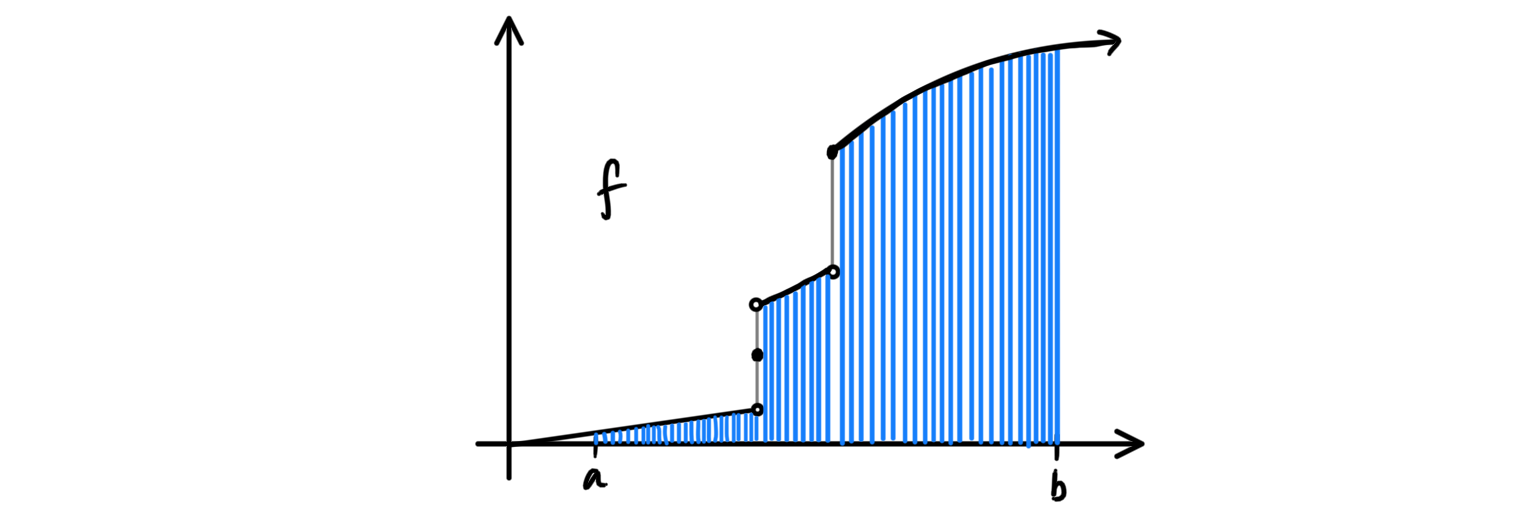
\includegraphics[scale=0.25]{img/Integrability_of_Monotonic_Function.PNG}
    \end{center}
    \end{corollary}

    \begin{definition}[Upper, Lower Riemann Sums]
      Let $f: [a, b] \longrightarrow \mathbb{R}$ be a real-valued function that is defined and bounded on the closed interval $[a, b]$, and let $P$ be a partition of $[a, b]$, and let $\Delta_i$ ($i = 1, 2, \ldots, n$) be the intervals of the partition $P$. Let 
      \begin{align*}
          m_i &= \inf_{x \in \Delta_i} f(x) \\
          M_i &= \sup_{x \in \Delta_i} f(x)
      \end{align*}
      be the infimum and supremum of $f$ over $\Delta x_i$. Then, the sums
      \begin{align*}
          s(f; P) & \equiv \sum_{i = 1}^n m_i \, \Delta x_i \\
          S(f; P) & \equiv \sum_{i=1}^n M_i \, \Delta x_i
      \end{align*}
      are respectively called the \textbf{lower} and \textbf{upper Riemann sums} of the function $f$ on the interval $[a, b]$ corresponding to the partition $P$ of that interval. 

      Given an arbitrary partition $(P, \xi)$ with distinguished points on $[a, b]$, it is clear that
      \[s(f; P) = \inf_{\xi} \sigma(f; P, \xi) \leq \sigma(f; P, \xi) \leq \sup_{\xi} \sigma(f; P, \xi) = S(f; P)\]
    \end{definition}

    \begin{theorem}
    A bounded real-valued function $f: [a, b] \longrightarrow \mathbb{R}$ is Riemann integrable on $[a, b]$ if and only if the following limits exist and are equal to each other. 
    \[\underline{I} \equiv \lim_{\lambda(P) \rightarrow 0} s(f; P) = \lim_{\lambda(P) \rightarrow 0} S(f; P) \equiv \overline{I}\]
    When the relation is true, then the integral is this common value. 
    \[\int_a^b f(x) \,dx = \underline{I} = \overline{I}\]
    \end{theorem}

    Note that this condition of the upper and lower Riemann sums converging to the same value and the condition that 
    \[\lim_{\lambda(P) \rightarrow 0} \sum_{i = 1}^n \omega (f; \Delta_i) \, \Delta x_i = 0\]
    are the same. For we can see that the rectangles visualized from the equation above are the exact same rectangles formed by $S(f; P) - s(f; P)$! 
    \begin{center}
        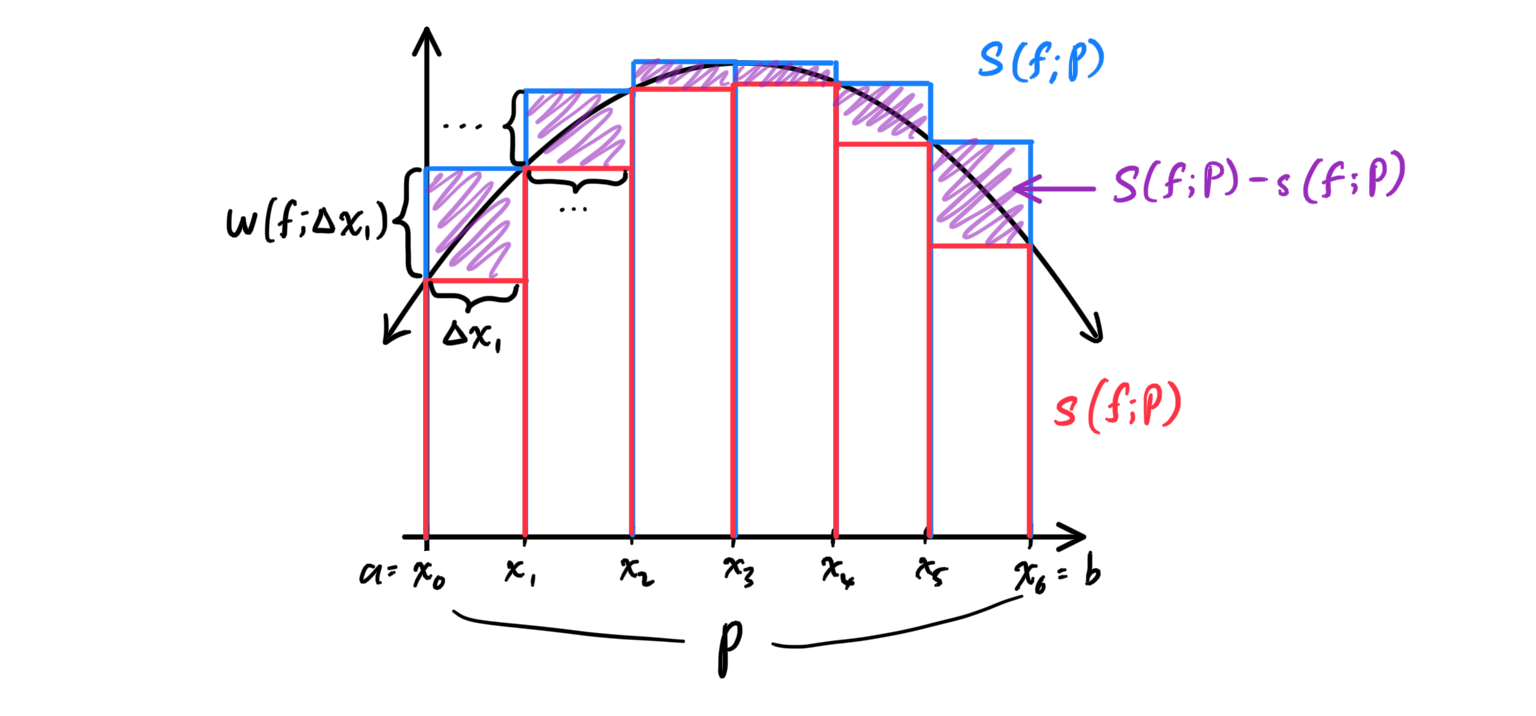
\includegraphics[scale=0.3]{img/Equivalent_Conditions_for_Integrability.PNG}
    \end{center}

    \subsubsection{The Vector Space of Riemann Integrable Functions}

    \begin{theorem}[The Vector Space of Integrable Functions]
    The set of Riemann integrable functions $\mathcal{R}[a, b]$ over closed interval $[a, b]$ is a vector space. That is, given $f, g \in \mathcal{R}[a, b]$ and $\alpha \in \mathbb{R}$, then
    \begin{enumerate}
      \item $(f + g) \in \mathcal{R}[a, b]$ 
      \item $(\alpha f) \in \mathcal{R}[a, b]$
    \end{enumerate}
    Furthermore, 
    \begin{enumerate}
      \item $|f| \in \mathcal{R}[a, b]$
      \item The restriction of $f$ in any $[c, d] \subset [a, b]$, denoted $f \big|_{[c,d]}$, is in $\mathcal{R}[c,d]$
      \item $(f \cdot g) \in \mathcal{R}[a, b]$
    \end{enumerate}
    \end{theorem}
    \begin{proof}

    \end{proof}

    \subsubsection{Lebesgue's Criterion for Riemann Integrability}
    We give Lebesgue's version of an intrinsic description of a Riemann integrable function. 

    \begin{definition}[Measure]
      A set $E \subset \mathbb{R}$ has \textbf{(Lebesgue) measure zero} if for every number $\epsilon > 0$ there exists a covering of the set $E$ be an at most countable system $\{I_k\}$ of intervals, the sum of whose lengths 
      \[\sum_{k=1}^\infty |I_k| \leq \epsilon\]
      This means that the above series summing up the lengths of the intervals is an absolutely convergent series. 
    \end{definition}

    \begin{lemma}
      We can deduce measures of basic sets. 
      \begin{enumerate}
        \item A finite number of points are sets of measure zero. 
        \item The union of a finite or countable number of sets of measure zero is a set of measure zero. \item A subset of a set of measure zero is itself a set of measure zero. 
        \item A closed interval $[a, b]$ with $a<b$ is not a set of measure zero. 
      \end{enumerate}
    \end{lemma}

    \begin{definition}
      If a property holds at all points of a set $X$ except possible the points of a set of measure zero, we say that this property holds \textbf{almost everywhere on $X$} or \textbf{at almost every point of $X$}. 
    \end{definition}

    Now, we can state Lebesgue's criterion for integrability, which nicely summarizes what we have so far. 

    \begin{theorem}[Lebesgue's Criterion for Integrability]
    A function defined on a closed interval is Riemann integrable on that interval if and only if it is bounded and continuous at almost every point. 
    \end{theorem}

    \begin{example}[Non-Integrability of the Dirichlet Function]
    The Dirichlet function
    \[\mathcal{D}(x) \equiv \begin{cases}
    1, & \text{ for } x \in \mathbb{Q} \\
    0, & \text{ for } x \in \mathbb{R} \setminus \mathbb{Q}
    \end{cases}\]
    on the interval $[0,1]$ is not integrable on that interval. We state two different reasons why. 
    \begin{enumerate}
      \item For any partition $P$ of $[0,1]$ we can find in each interval $\Delta_i$ both a rational point $\xi^\prime_i$ and an irrational point $\xi_i^{\prime\prime}$. Then, we can see that the lower and upper Riemann sums do not necessarily converge to each other since
      \[\sigma(f; P, \xi^\prime) = \sum_{i=1}^n 1 \cdot \Delta x_i = 1 \text{ while } \sigma(f;P, \xi^{\prime\prime}) = \sum_{i=1}^n 0 \cdot \Delta x_i = 0\]
      as $\lambda(P) \rightarrow 0$. 
      \item From the point of view of the Lebesgue criterion the nonintegrability of the Dirichlet function is obvious since $\mathcal{D}(x)$ is discontinuous at every point of $[0, 1]$, which is not a set of measure zero. 
    \end{enumerate}
    \end{example}

    Notice that by the Lebesgue criterion, integrability is a weaker condition than continuity. That is, 
    \[f \text{ continuous } \implies f \text{ Riemann integrable}\]
    but not necessarily the other way around. It turns out that this has consequences when determining the composition of functions. 

    \begin{proposition}[Integrable + Continuous Composition]
    Let $f: I_1 = [a, b] \longrightarrow\mathbb{R}$ be a function that is integrable on $[a, b]$, with Im$\,f = [c, d] = I_2$. Define a continuous (remember, continuity is stronger than integrability) function $g: [c, d] \longrightarrow \mathbb{R}$. Then the composition
    \[g \circ f: [a, b] \longrightarrow \mathbb{R}\]
    is clearly defined and continuous at all the points of $[a, b]$ where $f$ is continuous. But since $f$ is integrable, the union of all the discontinuities in $[a, b]$ must have measure zero, and so it follows that since $[a, b]$ is the same  
    \[g \circ f \in \mathcal{R}[a, b]\]
    Therefore, we can found out that 
    \[f \text{ integrable and } g \text{ continuous} \implies g \circ f \text{ integrable}\]
    as visualized in the commutative diagram below. 
    \[
      \begin{tikzcd}
        I_1 \arrow[r, "f"] \arrow[rr, bend left, "g \circ f"] & I_2 \arrow[r, "g"] & \mathbb{R}
      \end{tikzcd}
    \]
    However, contrary to intuition, 
    \[f \text{ integrable and } g \text{ integrable} \centernot\implies g \circ f \text{ integrable}\]
    \end{proposition}

    We present a counterexample. 
    \begin{example}
    Consider the functions
    \[|sgn|(x) \equiv \begin{cases}
    1 & x \neq 0 \\
    0 & x = 0
    \end{cases}\]
    and the Riemann function 
    \[\mathcal{R}(x) \equiv \begin{cases}
    \frac{1}{n} & x = \frac{m}{n} \in \mathbb{Q}, \gcd(m, n) = 1 \\
    0 & x \in \mathbb{R} \setminus \mathbb{Q}
    \end{cases}\]
    We can see that $\mathcal{R}$ is continuous at all irrational points and discontinuous at all rational points except $0$, meaning that it is integrable ($\mathbb{Q}$ has measure zero). Then, the composition of these two functions is precisely the Dirichlet function
    \[\mathcal{D}(x) = |sgn| \circ \mathcal{R}\]
    which is not integrable. 
    \end{example}

  \subsection{Basic Properties of the Integral}

    One of the most basic properties of the integral is that it is a linear map. 
    \begin{lemma}[Linearity of the Integral]
      Given closed interval $[a, b] \subset \mathbb{R}$, the Riemann integration function 
      \[\int_a^b: \mathcal{R}[a, b] \longrightarrow \mathbb{R}\]
      is a linear functional living within the dual space $\mathbb{R}^* [a, b]$. That is, given $f, g \in \mathcal{R}[a, b]$, a linear combination of them $\alpha f + \beta g$ is also integrable on $[a,b]$, and 
      \[\int_a^b (\alpha f + \beta g)(x)\,dx = \alpha \int_a^b f(x)\,dx + \beta \int_a^b g(x)\,dx\]
    \end{lemma}
    \begin{proof}
    It is clear from basic algebraic transformation that the Riemann sums for the integral expressions on both sides are equal. 
    \[\sum_{i=1}^n (\alpha f + \beta g) (\xi_i) \Delta x_i = \alpha \sum_{i=1}^n f(\xi_i) \Delta x_i + \beta \sum_{i=1}^n g(\xi_i) \Delta x_i\]
    Taking the limit as $\lambda(P) \rightarrow 0$ on both sides leads to the respective Riemann integrals. 
    \end{proof}


    The next property of the Riemann integral is its additive property \textbf{on the interval of integration}. Note that the value of the integral 
    \[\int_a^b f(x) \,dx \equiv \lim_{\lambda(P) \rightarrow 0} \sigma(f; P, \xi)\]
    depends on both the integrand and the closed interval over which the integral is taken. 

    \begin{lemma}[Properties of the Interval of Integration]
      If $a < b < c$ and $f \in \mathcal{R}[a, c]$, then $f \big|_{[a,b]} \in \mathcal{R}[a, b]$, $f \big|_{[b,c]} \in \mathcal{R}[b, c]$, and the following equality holds 
      \[\int_a^c f(x)\,dx = \int_a^b f(x)\, dx + \int_b^c f(x)\,dx\]
      From these we set
      \[\int_a^b f(x)\,dx \equiv - \int_b^a f(x)\,dx\]
      and 
      \[\int_a^a f(x)\,dx \equiv 0\]
    \end{lemma}

    \begin{theorem}[Symmetry of the Riemann Integral]
    Let $a, b, c \in \mathbb{R}$ and let $f$ be integrable over the largest closed interval having two of these points as endpoints. Then, the restriction of $f$ to each of the other closed intervals is also integrable over those intervals and the following equality holds. 
    \[\int_a^b f(x)\,dx + \int_b^c f(x)\,dx + \int_c^a f(x)\,dx = 0\]
    This property can be abstractified to those of additive interval functions, which will be shown soon. 
    \end{theorem}

    We finally end with an important property of the integral which, as seen later, allows us to define inner products on function spaces. 
    \begin{theorem}
    If $a \leq b$ and $f \in \mathcal{R}[a, b]$, then $|f| \in \mathcal{R}[a, b]$, and 
    \[\Bigg| \int_a^b f(x)\,dx \Bigg| \leq \int_a^b |f|(x)\,dx\]
    \end{theorem}

    \subsubsection{Mean Value Theorem of the Integral}

    \begin{lemma}[Monotonicity of the Integral]
      If $a \leq b, f_1, f_2 \in \mathcal{R}[a, b]$, and $f_1 (x) \leq f_2 (x)$ for every $x \in [a, b]$, then
      \[\int_a^b f_1 (x)\,dx \leq \int_a^b f_2 (x)\,dx\]
      \begin{center}
          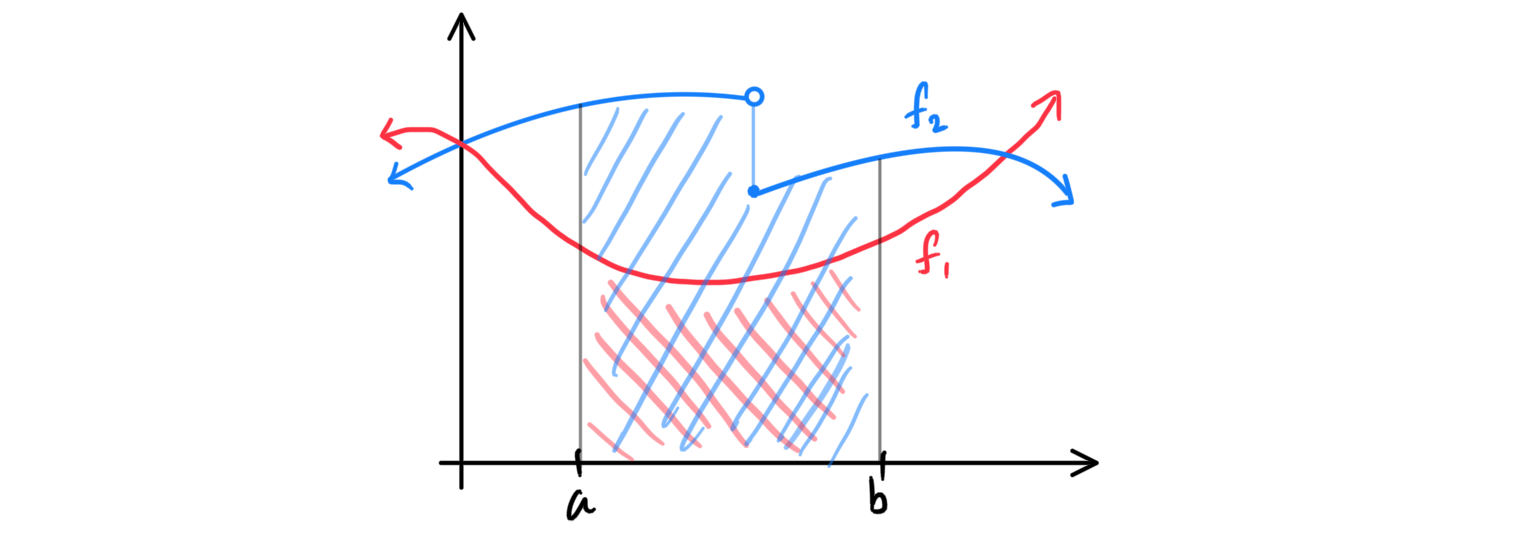
\includegraphics[scale=0.27]{img/Monotonicity_of_Integral.PNG}
      \end{center}
      This immediately implies that given constants $m, M$ such that $m \leq f(x) \leq M$ at each $x \in [a, b]$, we have
      \[m \cdot (b - a) \leq \int_a^b f(x)\,dx \leq M \cdot (b-a)\]
      This is very easily visualized below. 
      \begin{center}
          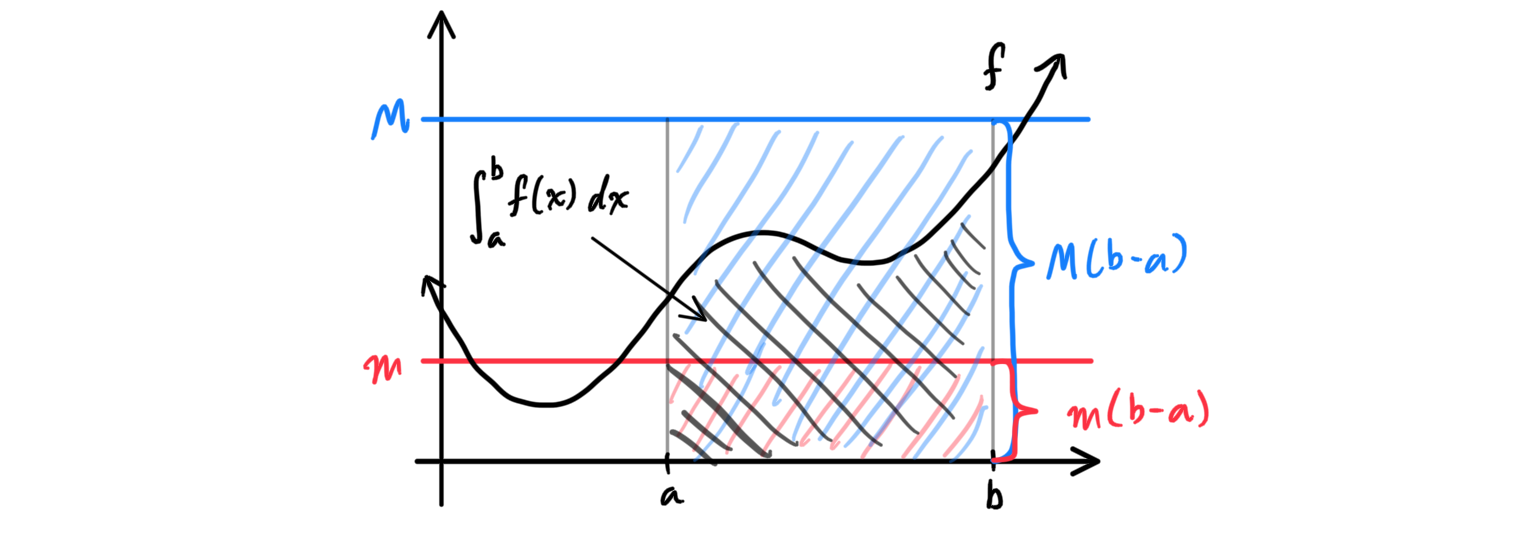
\includegraphics[scale=0.27]{img/Monotonicity_of_Intergral_2.PNG}
      \end{center}
      In particular, if $0 \leq f(x)$ on $[a, b]$, then
      \[0 \leq \int_a^b f(x)\,dx\]
    \end{lemma}

    \begin{theorem}[Mean Value Theorem of the Integral]
    Given $f \in \mathcal{R}[a, b]$, with 
    \[m = \inf_{x \in [a, b]} f(x) \text{ and } M = \sup_{x \in [a, b]} f(x)\]
    then there exists a number $\mu \in [m, M]$ such that
    \[\int_a^b f(x)\,dx = \mu \cdot (b - a)\]
    Furthermore, if $f \in C[a, b]$ (that is, continuous on $[a, b]$), it immediately follows by the intermediate value theorem that there exists a point $\xi \in [a, b]$ such that
    \[\int_a^b f(x)\,dx = f(\xi) (b - a)\]
    \begin{center}
        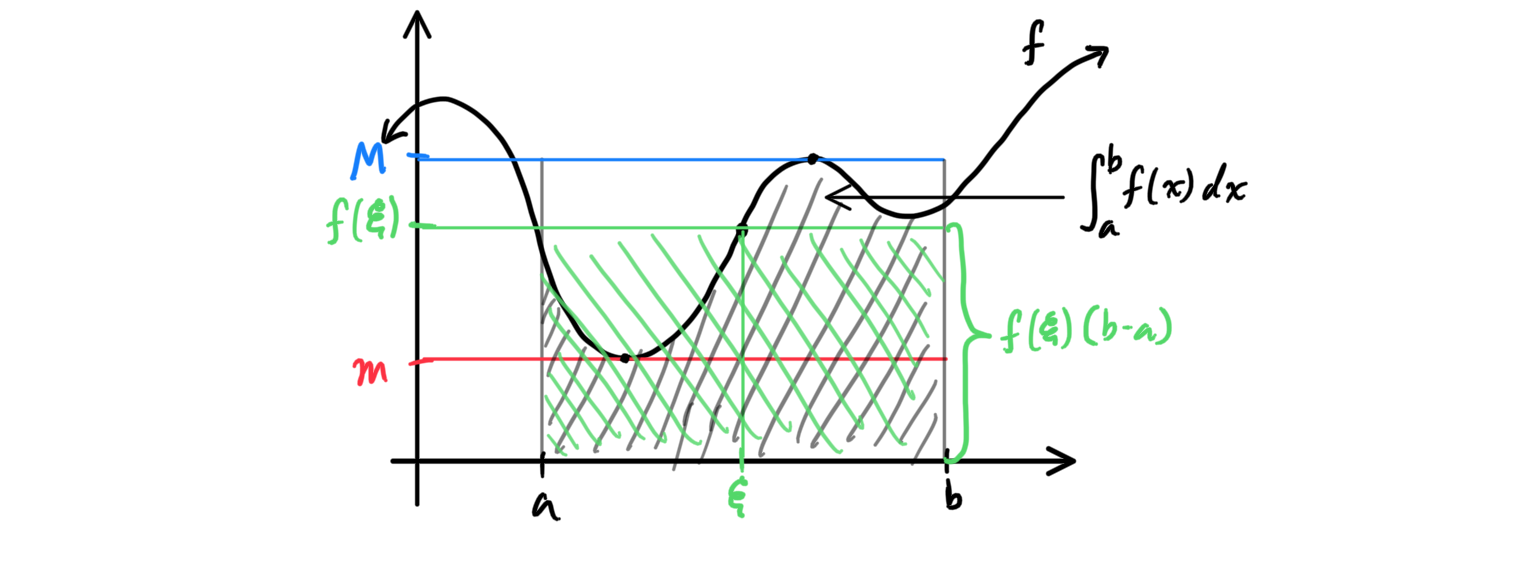
\includegraphics[scale=0.27]{img/Mean_Plus_Intermediate_Value_Theorem_Integral.PNG}
    \end{center}
    \end{theorem}

    Due to the length of the proof, we ask the reader to take it for granted the following theorem. 

    \begin{theorem}[Bonnet's Formula]
    If $f, g \in \mathcal{R}[a, b]$ and $g$ is a monotonic function on $[a, b]$, then there exists a point $\xi \in [a, b]$ such that
    \[\int_a^b (f \cdot g) (x)\,dx = g(a) \int_a^\xi f(x)\,dx + g(b) \int_\xi^b f(x)\,dx\]
    \end{theorem}

  \subsection{Connections between Integrals, Primitives, Derivatives}

    \begin{definition}[Integral with Variable Upper Limit]
      Let $f \in \mathcal{R}[a, b]$, and let us choose an $x \in [a, b]$ in order to construct the function
      \[F(x) \equiv \int_a^x f(t)\,dt\]
      which is called an \textbf{integral with variable upper limit}. Note that since $[a, x] \subset [a, b]$, it follows that $f \big|_{[a,x]} \in \mathcal{R}[a, x]$ and therefore the function $x \mapsto F(x)$ is unambiguously defined for $x \in [a, b]$. 
      \begin{center}
          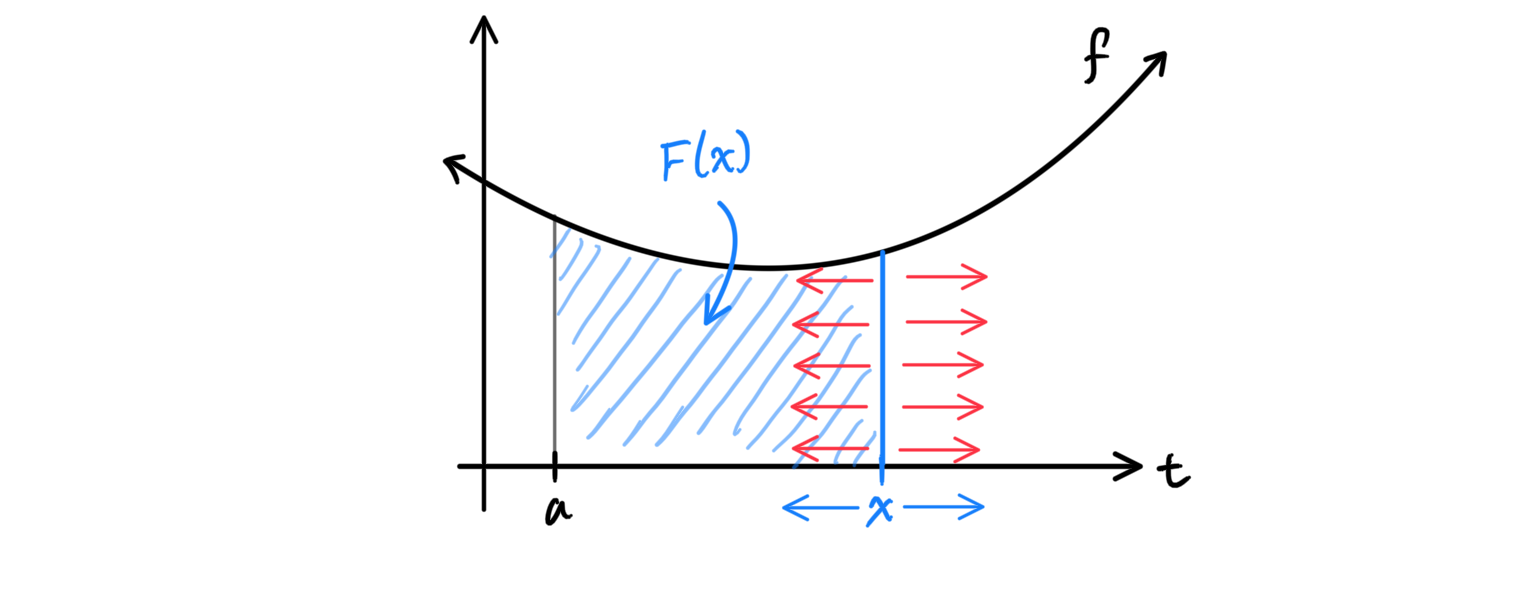
\includegraphics[scale=0.27]{img/Integral_with_Variable_Upper_Limit.PNG}
      \end{center}
      Furthermore, $F(x)$ is continuous on $[a, b]$. Since $f$ is integrable on $[a, b]$, it is bounded by a constant $C$ such that
      \[|f(t)| \leq C \text{ on } [a, b]\]
      It follows from the additive properties of the integral and boundedness theorem that 
      \[|F(x + h) - F(x)| \leq C|h|\]
      if $x, x + h \in [a, b]$, as visualized. This means that for any $\delta$-neighborhood of $F(x)$, we can find an arbitrary small $h$ such that the $C|h|$-neighborhood of $F(x)$ is completely contained in the $\delta$-neighborhood. But by the inequality above, this means that there exists an $\epsilon = h$-neighborhood of $x$ such that its entire image is contained within the $C|h|$-neighborhood, which itself is contained within the $\delta$-neighborhood. This shows that $F$ is continuous. 
    \end{definition}

    \begin{theorem}[First Fundamental Theorem of Calculus]
    Let $f \in \mathcal{R}[a, b]$ be continuous at point $x \in [a, b]$ (resp. continuous on closed interval $[a, b]$). Let $F$ be the function, defined for all $x \in [a, b]$ by 
    \[F(x) \equiv \int_a^x f(t)\,dt\]
    Then, $f$ is continuous and differentiable at $x$ (resp. uniformly continuous on $[a, b]$ and differentiable on $(a, b)$), 
    \[F^\prime (x) = f(x)\]
    at $x$ (resp. for all $x \in [a, b]$). This is an amazing fact, because visually, it tells us that the rate at which the integral $F$ is increasing at $x$ (represented by the increasing area under the curve of $f$) is equal to the value of $f$ at the point $x$ itself! 
    \begin{center}
        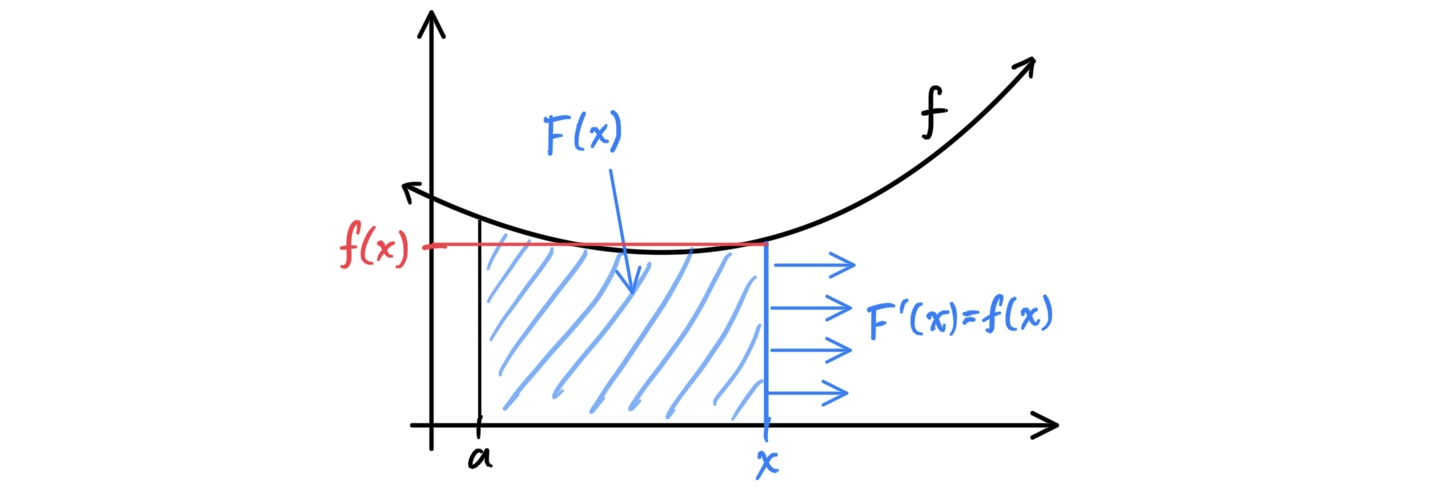
\includegraphics[scale=0.25]{img/First_Fundamental_Theorem_Analysis.jpg}
    \end{center}
    \end{theorem}
    \begin{proof}
    Let $x, x + h \in [a, b]$, and let us estimate the difference $F(x+h) - F(x)$. It follows from the continuity of $f$ at $x$ that $f(t) = f(x) + \Delta(t)$, where $\Delta(t) \rightarrow 0$ as $t \rightarrow x$. If point $x$ is held fixed, the function 
    \[\Delta(t) = f(t) - f(x)\]
    is integrable on $[a, b]$, being the difference of the integrable function $t \mapsto f(t)$ and the constant $f(x)$. Let us denote
    \[M(h) \equiv \sup_{t \in [x, x+h]} |\Delta(t)|\]
    which means that $M(h)$ is the largest difference between $f(x)$ and $f(t)$ in the interval $[x, x+h]$. 
    \begin{center}
        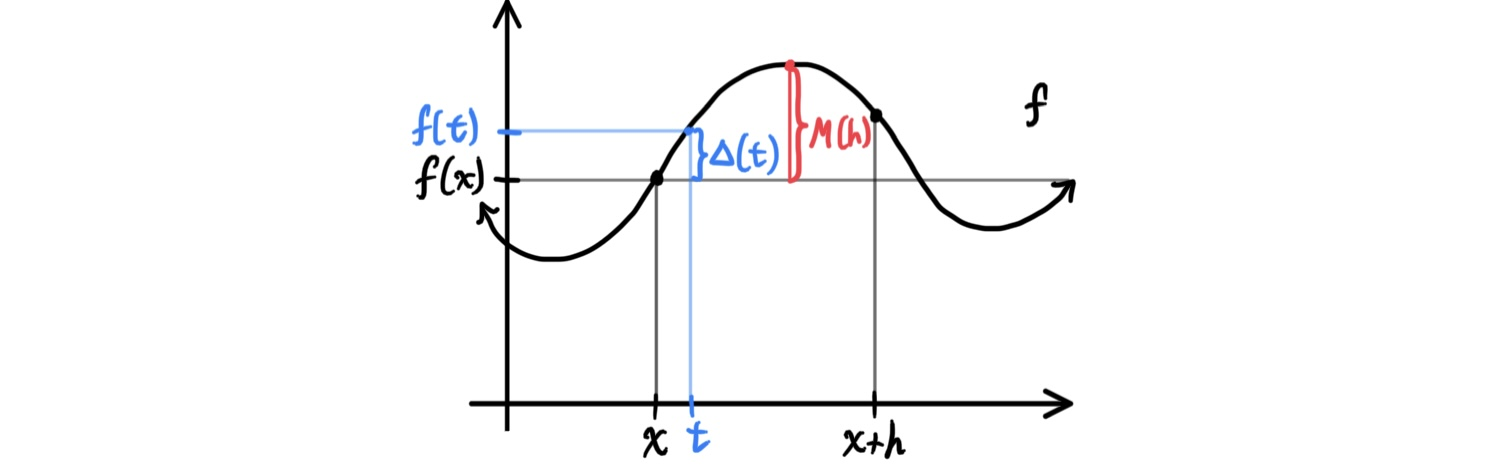
\includegraphics[scale=0.25]{img/Proof_First_Fundamental_Theorem_Analysis.jpg}
    \end{center}
    Clearly $M(h) \rightarrow 0$ as $h \rightarrow 0$. We can now find
    \begin{align*}
        F(x + h) - F(x) & = \int_a^{x+h} f(t)\,dt - \int_a^x f(t)\,dt \\
        & = \int_x^{x+h} f(t)\,dt \\
        & = \int_x^{x+h} \big( f(x) + \Delta(t)\big)\,dt \\
        & = \int_x^{x+h} f(x)\,dt + \int_x^{x+h} \Delta(t)\,dt \\
        & = f(x) h + \alpha(h) h
    \end{align*}
    where we have set 
    \[\int_x^{x+h} \Delta(t)\,dt = \alpha(h) h\]
    where $\alpha$ is infinitesimal as $h \rightarrow 0$, since 
    \[\Bigg| \int_x^{x+h} \Delta(t)\,dt \Bigg| \leq \Bigg| \int_x^{x+h} |\Delta(t)|\,dt \Bigg| \leq \Bigg| \int_x^{x+h} M(h)\,dt \Bigg| = M(h) |h| = \alpha(h)|h|\]
    Therefore, we have shown that if the function $f$ is continuous at a point $x \in [a, b]$, then for displacements $h$ from $x$ such that $x +h \in [a, b]$, the following equality holds.
    \[F(x + h) - F(x) = f(x) h + \alpha(h) h\]
    where $\alpha(h) \rightarrow 0$ as $h \rightarrow 0$, and by definition, this means that $F(x)$ is differentaible on $[a, b]$ at the point $x \in [a, b]$ and that $F^\prime(x) = f(x)$. 
    \end{proof}

    \begin{corollary}
    Every bounded function $f: [a, b] \longrightarrow \mathbb{R}$ on the closed interval $[a, b]$ and has only a finite number of points of discontinuity has a primitive, and every primitive of $f$ on $[a, b]$ has the form 
    \[\mathcal{F}(x) \equiv \int_a^x f(t)\,dt + c\]
    where $c$ is a constant. 
    \end{corollary}

    \begin{theorem}[Second Fundamental Theorem of Calculus]
    Let $f$ be a real-valued function on a closed interval $[a, b]$ with $\mathcal{F}$ any primitive of $f$ on $[a, b]$. If $f$ is Riemann-integrable (i.e. $f$ bounded with finite points of Lebesgue measure zero) on $[a, b]$, then 
    \[\int_a^b f(x)\,dx  = \mathcal{F} \big|_a^b \equiv \mathcal{F}(b) - \mathcal{F}(a)\]
    \begin{center}
        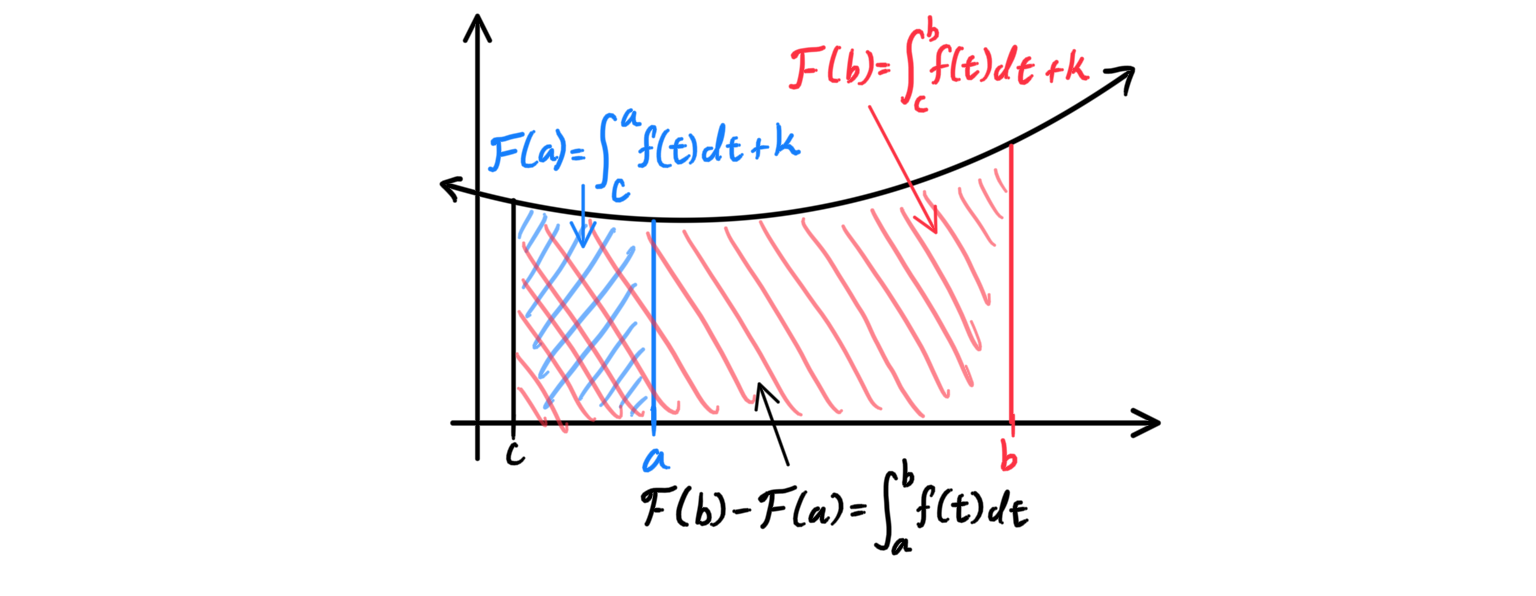
\includegraphics[scale=0.25]{img/Second_Fundamental_Theorem_Analysis.PNG}
    \end{center}
    \end{theorem}
    \begin{proof}
    We already know that a bounded function on a closed interval having a finite number of discontinuities is integrable, and by the corollary, we are guaranteed an existence of a primitive $\mathcal{F}(x)$ of the function $f$ on $[a, b]$ with the form 
    \[\mathcal{F} (x) \equiv \int_a^x f(t)\,dt + c\]
    Setting $x = a$, we find that $c = \mathcal{F}(a)$, and so 
    \[\mathcal{F}(x) \equiv \int_a^x f(t)\,dt + \mathcal{F}(a)\]
    Evaluating $\mathcal{F}$ at $x = b$ gives
    \[\int_a^b f(t)\,dt = \mathcal{F}(b) - \mathcal{F}(a)\]
    \end{proof}

    \subsubsection{Integration by Parts and Taylor's Formula}
    \begin{theorem}[Definite Integration by Parts]
    If the functions $u(x)$ and $v(x)$ are continuously differentiable on a closed interval with endpoints $a$ and $b$, then
    \[\int_a^b (u \cdot v^\prime)(x)\,dx = (u \cdot v)\big|^b_a - \int_a^b (v \cdot u^\prime)(x)\,dx\]
    which is customarily written in the form as
    \[\int_a^b u\,dv = u \cdot v \big|_a^b - \int_a^b v\,du\]
    \end{theorem}
    \begin{proof}
    By the product rule of differentiation, we have
    \[(u \cdot v)^\prime (x) = (u^\prime \cdot v)(x) + (u \cdot v^\prime) (x)\]
    where by hypothesis, $u^\prime \cdot v, u \cdot v^\prime$ are continuous and hence integrable on $[a, b]$. Using the linearity of the integral and the 2nd fundamental theorem of calculus, we get
    \[(u \cdot v) (x) \big|^b_a = \int_a^b (u^\prime \cdot v)(x)\,dx + \int_a^b (u \cdot v^\prime) (x)\,dx\]
    \end{proof}

    \begin{theorem}[Integral Form of the Remainder]
    If $f: E \longrightarrow \mathbb{R}$ has continuous derivatives up to order $n$ on the closed interval $[a, x]$, then Taylor's formula holds
    \[f(x) = f(a) + \frac{f^\prime (a)}{1!} (x - a) + \ldots + \frac{f^{(n-1)}(a)}{(n-1)!} (x - a)^{n-1} + r_{n-1}(a; x)\]
    where 
    \[r_{n-1} (a;x) = \frac{1}{(n-1)!} \int_a^x f^{(n)} (t) (x - t)^{n-1} \,dt\]
    This form is called \textbf{Taylor's formula with the integral form of the remainder}. 
    \end{theorem}
    \begin{proof}
    Using the 2nd fundamental theorem and the definite integration by parts formula, we can carry out the following chain of transformations, assuming continuity and differentiability when needed. 
    \begin{align*}
        f(x) - f(a) & = \int_a^x f^\prime (t) \,dt \\
        & = - \int_a^x f^\prime(t) (x - t)^\prime \,dt \\
        & = -f^\prime (t) (x - t)\big|_a^x + \int_a^x f^{\prime\prime} (t) (x - t) \,dt \\
        & = f^\prime (a) (x - a) - \frac{1}{2} \int_a^x f^{\prime\prime} (t) \big( (x - t)^2\big)^\prime \,dt \\
        & = f^\prime (x - a) - \frac{1}{2} f^{\prime\prime} (t) (x - t)^2 \big|_a^x + \frac{1}{2} \int_a^x f^{\prime\prime\prime} (t) (x - t)^2\,dt \\
        & = f^\prime(a) (x - a) + \frac{1}{2} f^{\prime\prime} (a) (x - a)^2 - \frac{1}{2 \cdot 3} \int_a^x f^{\prime\prime\prime} (t) \big((x - t)^3\big)^\prime\,dt \\
        & = \ldots \\
        & = f^\prime (a) (x - a) + \ldots + \frac{1}{(n-1)!} f^{(n-1)} (a)(x - a)^{n-1} + r_{n-1}(a;x)
    \end{align*}
    where $r_{n-1}(a;x)$ is given by the integral formula mentioned. 
    \end{proof}

    \subsubsection{Change of Variables in Integration}
    We now show and prove the method what we call "u-substitution" for definite integration. 

    \begin{theorem}[Change of Variable]
    If $\varphi: [\alpha, \beta] \longrightarrow [a, b]$ is a continuously differentiable mapping such that $\varphi(\alpha) = a$ and $\varphi(\beta) = b$, then for any continuous function $f(x)$ on $[a, b]$ the function $f\big(\varphi(t)\big) \varphi^\prime (t)$ is continuous on the closed interval $[\alpha, \beta]$ and 
    \[\int_a^b f(x)\,dx = \int_\alpha^\beta f\big(\varphi(t)\big) \varphi^\prime(t)\,dt\]
    \begin{center}
        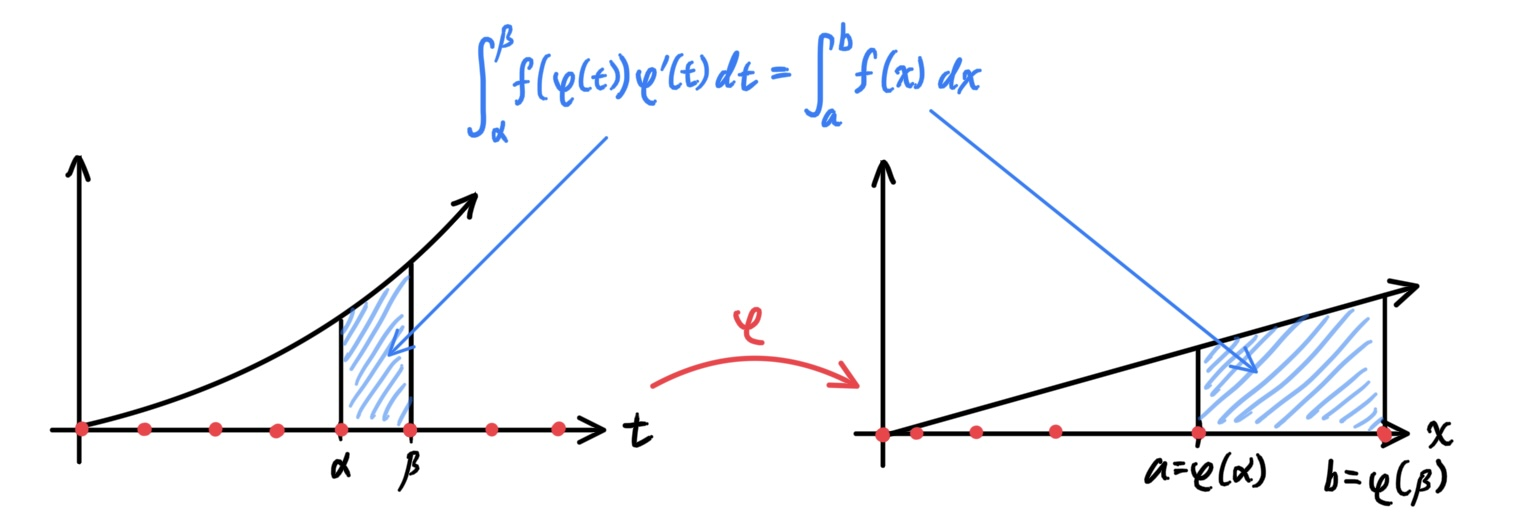
\includegraphics[scale=0.25]{img/Change_of_Variable_Analysis_Integral.jpg}
    \end{center}
    \end{theorem}
    \begin{proof}
    We prove a slightly weaker form of the theorem with the additional hypothesis that $\varphi$ is strictly monotonic. 
    \end{proof}

    \subsubsection{Additive Interval Functions and the Integral}
    In this section we take a step back and construct the integral in a more abstract sense, using the concepts of an additive interval function. 

    \begin{definition}[Additive Interval Function]
      An \textbf{additive (oriented) interval function} is a function 
      \[(\alpha, \beta) \mapsto I(\alpha, \beta) \in \mathbb{R}\]
      that assigns a number $I(\alpha, \beta)$ to each ordered pair of points $(\alpha, \beta)$ of a fixed closed interval $[a, b]$ in such a way that the following equality holds for any triple of points $\alpha, \beta, \gamma \in [a, b]$. 
      \[I(\alpha, \gamma) = I(\alpha, \beta) + I(\beta, \gamma)\]
      Notice that the integral holds this property, shown in the theorem on the symmetric property of the integral. It follows that all additive interval functions are anticommutative: 
      \[I(\alpha, \beta) + I(\beta, \alpha) = 0\]
      which immediately results in
      \[I(\alpha, \alpha) = 0\]
    \end{definition}

    \begin{lemma}[Generating Functions of Additive Interval Functions]
      For any function $x \mapsto \mathcal{F}(x)$ that maps points on the interval $[a, b]$ to $\mathbb{R}$, we set
      \[\mathcal{F}(x) \equiv I(a, x)\]
      and by additivity we have
      \[I(\alpha, \beta) = I(\alpha, \beta) - I(a, \alpha) = \mathcal{F}(\beta) - \mathcal{F}(\alpha)\]
      and thus, every additive oriented interval function has the form 
      \[I(\alpha, \beta) = \mathcal{F}(\beta) - \mathcal{F}(\alpha)\]
      By constructing $I$ in this manner, we say that \textbf{the function $\mathcal{F}$ generates the additive function $I$}. 
    \end{lemma}

    \begin{example}
    If $f \in \mathcal{R}[a, b]$, the function $\mathcal{F} = \int_a^x f(t)\,dt$ generates the additive function
    \[I(\alpha, \beta) = \mathcal{F}(\beta) - \mathcal{F}(\alpha) = \int_a^\beta f(t)\,dt - \int_a^\alpha f(t)\,dt = \int_\alpha^\beta f(t)\,dt\]
    \end{example}

    We conclude by stating a sufficient condition for an additive interval function to be generated by an integral. 
    \begin{theorem}
    Suppose the additive function $I(\alpha, \beta)$ defined for points $\alpha, \beta \in [a, b]$ has the property that, for some known function $f \in \mathcal{R}[a, b]$, 
    \[\inf_{x \in [\alpha, \beta]} f(x) (\beta - \alpha) \leq I(\alpha, \beta) \leq \sup_{x \in [\alpha, \beta]} f(x) (\beta - \alpha)\]
    holds for any closed interval $[\alpha, \beta] \subset [a, b]$ ($\alpha \leq \beta$). Then, the additive function $I$ must be the definite integral
    \[I(a, b) = \int_a^b f(x)\,dx\]
    \end{theorem}

    This theorem is extremely useful. It says that if we have any abstract additive interval function $I(\alpha, \beta)$ that satisfies the properties above, then it \textbf{must} be generated by an integral with variable upper limit, meaning that (by the previous example) $I$ itself must be a definite integral! 

    \subsubsection{Arc Length}
    When modeling systems in physics, one of the most fundamental tools we use are path functions that models the movement of a particle in $\mathbb{R}^3$. 

    \begin{definition}[Path]
      A \textbf{path} in $\mathbb{R}^3$ is a continuous mapping $r: [a, b] \subset \mathbb{R} \longrightarrow \mathbb{R}^3$ defined
      \[t \mapsto \big(x(t), y(t), z(t)\big)\]
      of an interval of the real line into $\mathbb{R}^3$ defined by the (continuous) scalar functions $x, y, z$. The endpoints 
      \[A = \big(x(a), y(a), z(a)\big) \text{ and } B = \big(x(b), y(b), z(b)\big)\]
      in $\mathbb{R}^3$ are called the \textbf{initial point} and \textbf{terminal point} of the path. Furthermore, a path is \textbf{closed} if its initial and terminal points coincide. 
    \end{definition}

    \begin{definition}[Support]
      If $\Gamma: I \longrightarrow \mathbb{R}^3$ is a path, the image $\Gamma(I) \subset \mathbb{R}^3$ is called the \textbf{support} of the path. 
    \end{definition}

    \begin{definition}[Simple Paths]
      A path $\Gamma: I \longrightarrow \mathbb{R}^3$ that is injective is called a \textbf{simple path}, or a \textbf{paramaterized curve}, and its support is called a \textbf{curve} in $\mathbb{R}^3$. 

      A closed path $\Gamma: [a, b] \longrightarrow \mathbb{R}^3$ is called a \textbf{simple closed path/curve} if the path $\Gamma: [a, b) \longrightarrow \mathbb{R}^3$ is simple. 
    \end{definition}

    \begin{definition}[Smooth Paths]
      A path $\Gamma: [a, b] \longrightarrow \mathbb{R}^3$ is $C^k$ smooth if the functions $x(t), y(t), z(t)$ are $C^k$ smooth. $\Gamma$ is \textbf{piecewise smooth} if the closed interval $[a, b]$ can be partitioned into a finite number of closed intervals on each of which the corresponding restriction of $\Gamma$ is smooth. 
    \end{definition}

    Now, we are ready to construct the length of a smooth path $\Gamma: [a, b] \longrightarrow \mathbb{R}^3$. Our initial ideas about the length $l[a, b]$ of the path traversed during the time interval $\alpha \leq t \leq \beta$ are as follows: 
    \begin{enumerate}
      \item If $\alpha < \beta < \gamma$, then $l$ is an additive interval function.
      \[l[\alpha, \gamma] = l[\alpha, \beta] + l[\beta, \gamma]\]
      \item If $v(t) = \big( x^\prime (t), y^\prime (t), z^\prime (t)\big)$ is the velocity of the point at time $t$, then 
      \[\int_{x \in [\alpha, \beta]} |v(t)| (\beta - \alpha) \leq l[\alpha, \beta] \leq \sup_{x \in [\alpha, \beta]} |v(t)| (\beta - \alpha)\]
    \end{enumerate}
    Thus, if the functions $x, y, z$ are continuously differentiable on $[a, b]$, this is sufficient condition (by the theorem in the previous subsection) that the additive function $l$ is an integral.

    \begin{definition}[Arc Length Integral]
      The length of a smooth path $\Gamma: [a, b] \longrightarrow \mathbb{R}^3$ is defined by 
      \[l[a, b] \equiv \int_a^b |\Gamma^\prime (t)|\,dt \equiv \int_a^b \sqrt{x^{\prime 2} (t) + y^{\prime 2} (t) + z^{\prime 2} (t)}\, dt\]
      We can visualize this by partitioning the interval $[a, b]$ into the intervals $\Delta_i$, each with point $\xi_i \in \Delta_i$. This would partition the path to $\Gamma(\Delta_i)$, each with points $\Gamma(\xi_i)$, and at each point $\Gamma(\xi_i)$, we can imagine the velocity vector of the curve. By taking the magnitude of this vector $\Gamma^\prime (\xi_i)$, we multiply it by the length of the interval $\Delta x_i$ to get one rectangle, creating an approximation for one partition of the path. 
      \begin{center}
          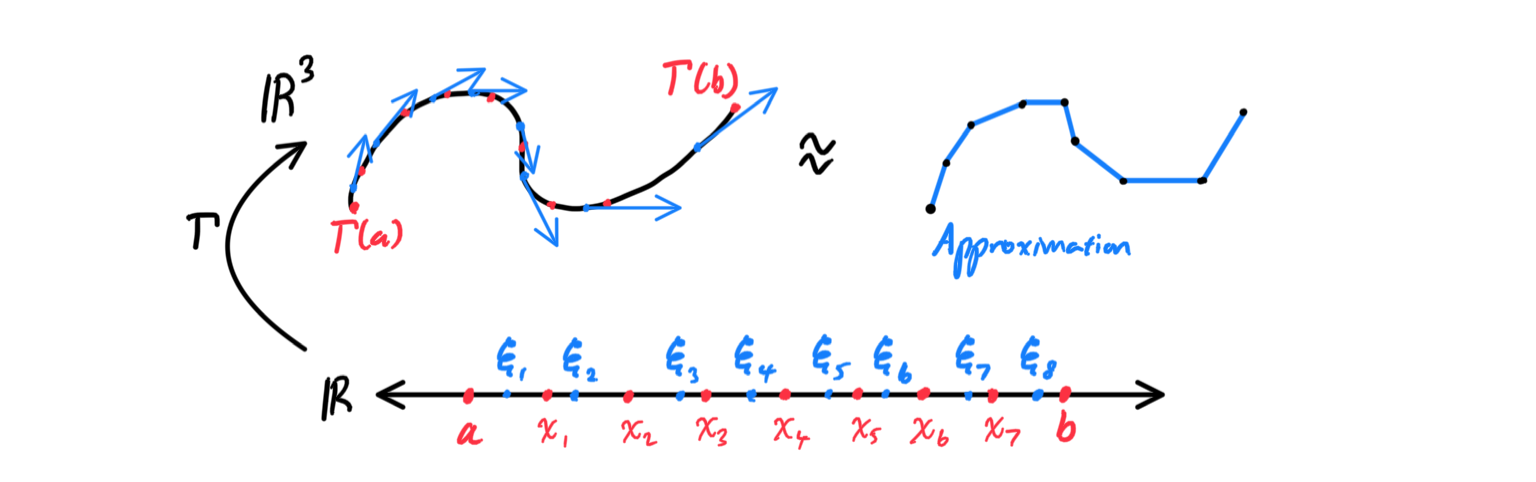
\includegraphics[scale=0.25]{img/Arc_Length_Integral.PNG}
      \end{center}
      An immediate result of this formula is the formula for the length of a graph of a function $f: [a, b] \longrightarrow \mathbb{R}$ in $\mathbb{R}^2$, by looking at the paramaterization $t \mapsto \Gamma(t) = \big(t, f(t)\big)$. 
      \[l[a,b] \equiv \int_a^b \sqrt{1 + (f^\prime (t))^2}\,dt\]
    \end{definition}

    The question on the effect of paramaterization on the integral now arises. 

    \begin{definition}[Admissible Change of Parameter]
      The path $\Tilde{\Gamma}: [\alpha, \beta] \longrightarrow \mathbb{R}^3$ is obtained from $\Gamma: [a, b] \longrightarrow \mathbb{R}^3$ by an \textbf{admissible change of parameter} if there exists a smooth mapping 
      \[T: [\alpha, \beta] \longrightarrow [a, b]\]
      such that $T(\alpha) = a, T(\beta) = b$, $T^\prime (\tau) > 0$ (that is, the reparamaterization $T$ is monotonic) on $[\alpha, \beta]$, and 
      \[\Tilde{\Gamma} = \Gamma \circ T\]
      The series of mappings can be represented with the following commutative diagram, where $I_{\alpha, \beta} = [\alpha, \beta] \subset \mathbb{R}$ and $I_{a, b} = [a, b] \subset \mathbb{R}$. 
      \[
        \begin{tikzcd}
          I_{\alpha, \beta} \arrow{r}{T} \arrow{rd}{\Tilde{\Gamma}}& I_{a, b} \arrow{d}{\Gamma}\\
           & \mathbb{R}^3
        \end{tikzcd}
      \]
      or with the more detailed visual below (Note that the points are labeled $0, 1, 2, 3, 4, 5$ do not represent numerical values, but rather the order in which the points are paramaterized. We can see from this ordering that $T$ is monotonic.)
      \begin{center}
          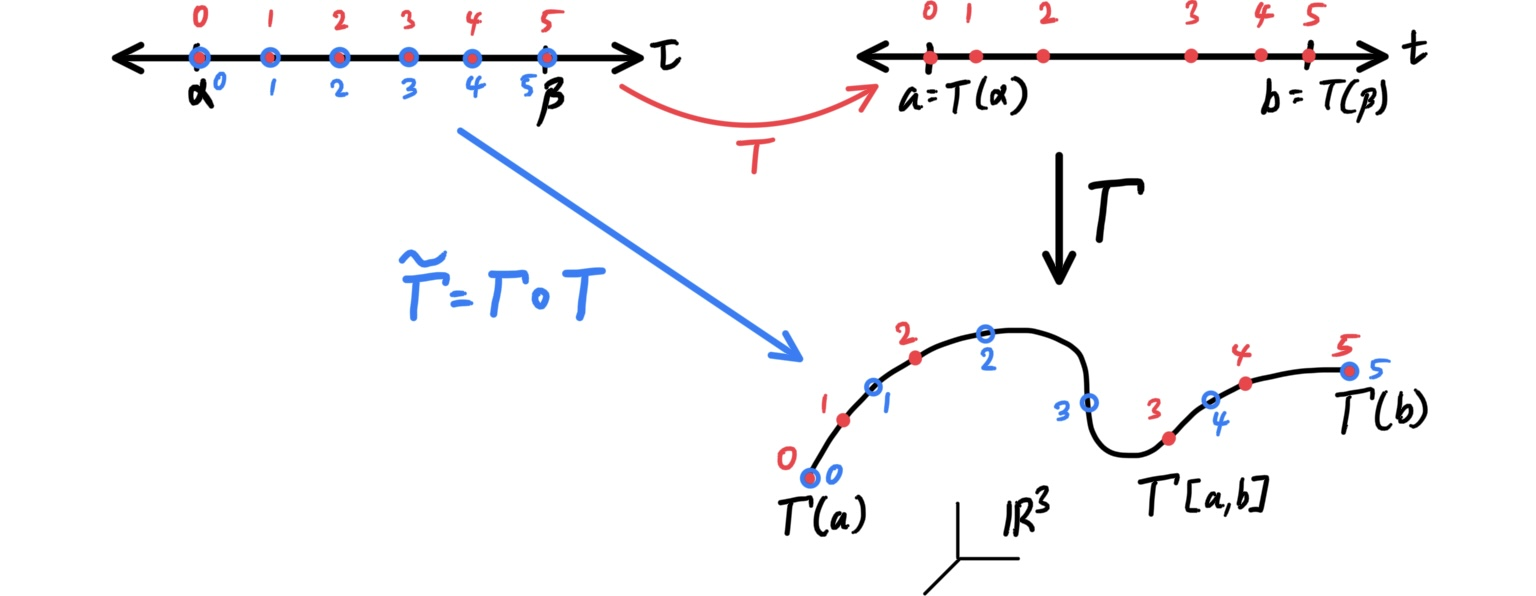
\includegraphics[scale=0.25]{img/Admissible_Change_of_Parameter.jpg}
      \end{center}
    \end{definition}

    \begin{theorem}[Invariance of Arclength Integral under Admissible Change of Parameters]
    If a smooth path $\Tilde{\Gamma}: [\alpha, \beta] \longrightarrow \mathbb{R}^3$ is obtained from a smooth path $\Gamma: [a, b] \longrightarrow \mathbb{R}^3$ by an admissible change of parameter, then the lengths of the two paths are equal. That is, a
    \[\int_a^b |\Gamma^\prime (t) |\,dt = \int_\alpha^\beta |\Tilde{\Gamma}^\prime (t)|\,dt \equiv \int_\alpha^\beta |(\Gamma \circ T)^\prime (t)|\,dt\]
    \end{theorem}

  \subsection{Improper Integrals}

    Due to some limitations of the Riemann integral, we cannot integrate over "singularities" where either the interval or the function is unbounded. We develop the tools of improper integration to deal with this problem; there are two types of improper integrals. 

    \begin{definition}[Improper Integral of Unbounded Interval]
      Suppose the function $x \mapsto f(x)$ is defined on the interval $[a, +\infty)$ and is integrable on every closed interval $[a, b]$ contained in that interval. Then, we call the following term
      \[\int_a^{+\infty} f(x)\,dx \equiv \lim_{b \rightarrow + \infty} \int_a^b f(x)\,dx\]
      the \textbf{improper Riemann integral of $f$ over the interval $[a, +\infty)$} and 
      \[\int_{-\infty}^b f(x)\,dx \equiv \lim_{a \rightarrow -\infty} \int_a^b f(x)\,dx \]
      the \textbf{improper Riemann integral of $f$ over the interval $(-\infty, b]$}.If the limit exists, then we say that the integral \textbf{converges} and \textbf{diverges} otherwise. 
    \end{definition}

    \begin{definition}[Improper Integral of Unbounded Function]
      Suppose the function $x \mapsto f(x)$ is defined on the interval $[a, B)$ and integrable on any closed interval $[a, b] \subset [a, B)$. Then, we call the following term
      \[\int_a^B f(x)\,dx \equiv \lim_{b \rightarrow B^-} \int_a^b f(x)\,dx\]
      the \textbf{improper Riemann integral of $f$ over interval $[a, B)$} and
      \[\int_A^b f(x)\,dx \equiv \lim_{a \rightarrow A^+} \int_a^b f(x)\,dx\]
      the \textbf{improper Riemann integral of $f$ over interval $(A,b]$}.
    \end{definition}

    For cohesiveness, we can combine these two definitions of improper integrals into the following one. 

    \begin{definition}[Improper Integrals]
      Let $[a, \omega)$ be a finite or infinite interval and $x \mapsto f(x)$ a function defined on that interval and integrable over every closed interval $[a, b] \subset [a, \omega)$. Then, by definition
      \[\int_a^\omega f(x)\,dx \equiv \lim_{b \rightarrow \omega} \int_a^b f(x)\,dx\]
      if this limit exists as $b \rightarrow \omega, b \in [a, \omega)$. Similarly, given the finite or infinite interval $(\omega, b]$ with $f$ integrable over every closed interval $[a, b] \subset (\omega, b]$, we have
      \[\int_\omega^b f(x)\,dx \equiv \lim_{a \rightarrow \omega} \int_a^b f(x)\,dx\]
      Note that if $\omega \in \mathbb{R}$ and $f \in \mathcal{R}[a, \omega]$, the improper integral is equivalent to the regular Riemann integral. 
      \[\int_a^\omega f(x) = \lim_{b\rightarrow \omega} \int_a^b f(x)\,dx\]
    \end{definition}

    \begin{lemma}[Properties of the Improper Integral]
      Suppose $f, g$ are functions defined on interval $[a, \omega)$ (without loss of generality, we let $\omega$ be the upper limit of integration) and integrable on every closed interval $[a, b] \subset [a, \omega)$. Suppose the improper integrals 
      \[\int_a^\omega f(x)\,dx \text{ and } \int_a^\omega g(x)\,dx\]
      are well-defined. 
      \begin{enumerate}
        \item For any $\lambda_1, \lambda_2 \in \mathbb{R}$ the function $(\lambda_1 f + \lambda_2 g)(x)$ is integrable in the improper sense on $[a, \omega)$ and
        \[\int_a^\omega (\lambda_1 f + \lambda_2 g)(x)\,dx = \lambda_1 \int_a^\omega f(x)\,dx + \lambda_2 \int_a^\omega g(x)\,dx\]
        \item For any $c \in [a, \omega)$, 
        \[\int_a^\omega f(x)\,dx = \int_a^c f(x)\,dx + \int_c^\omega f(x)\,dx\]
        \item If $\varphi: [\alpha, \gamma) \longrightarrow [a, \omega)$ is a smooth strictly monotonic mapping with $\varphi(\alpha) = a$ and $\varphi(\beta) \rightarrow \omega$ as $\beta \rightarrow \gamma^-$, then the improper integral of the function $t \mapsto (f \circ \varphi)(t) \varphi^\prime (t)$ over $[\alpha, \gamma)$ exists and 
        \[\int_a^\omega f(x)\,dx = \int_\alpha^\gamma (f \circ \varphi)(t) \varphi^\prime (t)\,dt\]
      \end{enumerate}
    \end{lemma}

    \subsubsection{Convergence of an Improper Integral}

      Note that by definition, an improper integral 
      \[\int_a^\omega f(x)\,dx \equiv \lim_{b \rightarrow \omega} \int_a^b f(x) \,dx\]
      is a limit of the function 
      \[\mathcal{F}(b) \equiv \int_a^b f(x)\,dx\]
      as $b \rightarrow \omega$. This means that we can use the Cauchy criterion to determine the convergence of this limit, and hence, existence of this improper integral. 

      \begin{theorem}[Cauchy Criterion for Convergence of an Improper Integral]
      If the function $x \mapsto f(x)$ is defined on the interval $[a, \omega)$ and integrable on every closed interval $[a, b] \subset [a, \omega)$, then the integral 
      \[\int_a^\omega f(x)\,dx\]
      converges if and only if for every $\epsilon > 0$ there exists $B \in [a, \omega)$ such that the relation
      \[\Bigg| \int_{b_1}^{b_2} f(x)\,dx \bigg| < \epsilon\]
      holds for any $b_1, b_2 \in [a, \omega)$ satisfying $B < b_1$ and $B < b_2$. 
      \end{theorem}
      \begin{proof}
      We have
      \[\int_{b_1}^{b_2} f(x)\,dx = \int_a^{b_2} f(x)\,dx - \int_a^{b_1} f(x)\,dx = \mathcal{F}(b_2) - \mathcal{F}(b_1)\]
      and therefore the condition is simply the Cauchy criterion for the existence of a limit for the function $\mathcal{F}(b)$ as $b \rightarrow \omega$. 
      \end{proof}

      \begin{definition}[Absolute Convergence of an Improper Integral]
        The improper integral 
        \[\int_a^\omega f(x)\,dx\]
        \textbf{converges absolutely} if the integral
        \[\int_a^\omega |f|(x)\,dx\]
        converges. Clearly, the inequality
        \[\Bigg| \int_{b_1}^{b_2} f(x)\,dx \Bigg| \leq \Bigg| \int_{b_1}^{b_2} |f|(x)\,dx \Bigg|\]
        implies that if an improper integral converges absolutely, then it converges. 
      \end{definition}

      This study of absolute convergence reduces to the study of convergence of integrals of nonnegative functions. The following lemma is useful in determining convergence of such functions. 

      \begin{lemma}
        Let there be a function $f$ defined on interval $[a, \omega)$ that is also integrable over every closed interval $[a, b] \subset [a, \omega)$. If $f(x) \geq 0$ on $[a, \omega)$, then the improper integral 
        \[\int_a^\omega f(x)\,dx\]
        exists if and only if the function 
        \[\mathcal{F}(b) \equiv \int_a^b f(x)\,dx\]
        is bounded on $[a, \omega)$. 
      \end{lemma}
      \begin{proof}
      It is clear that 
      \[\int_a^\omega f(x)\,dx = \lim_{b \rightarrow \omega} \mathcal{F}(b)\]
      If $f(x)\geq 0$, then the function $\mathcal{F}(b)$ is nondecreasing on $[a, \omega)$ and therefore has a limit as $b \rightarrow \omega$ only if it is bounded (since every monotonically increasing sequence that is bounded always converges). 
      \end{proof}

      This leads to the familiar integral test for convergence of a series. 

      \begin{theorem}[Integral Test for Convergence of a Series]
      If the function $x \mapsto f(x)$ is defined on the interval $[1, +\infty)$, nonnegative, nonincreasing, and integrable on each closed interval $[1, b] \subset [1, +\infty)$, then the series 
      \[\sum_{n=1}^\infty f(n) = f(1) + f(2) + \ldots\]
      and the integral 
      \[\int_a^{+\infty} f(x)\,dx\]
      either both converge or both diverge. 
      \end{theorem}

      We can use the comparison test analogue to determine convergence of improper integrals. 

      \begin{theorem}[Comparison Test for Convergence of Improper Integrals]
      Suppose the functions $f(x), g(x)$ are defined on the interval $[a, \omega)$ and integrable on any closed interval $[a, b] \subset [a, \omega)$. If 
      \[0 \leq f(x) \leq g(x)\]
      on $[a, \omega)$, then 
      \[\int_a^\omega g(x)\,dx \text{ converges} \implies \int_a^\omega f(x)\,dx \text{ converges}\]
      and the inequality 
      \[\int_a^\omega f(x)\,dx \leq \int_a^\omega g(x)\,dx\]
      holds. Also, 
      \[\int_a^\omega f(x)\,dx \text{ diverges} \implies \int_a^\omega g(x)\,dx \text{ diverges}\]
      \end{theorem}
    
    \subsubsection{Improper Integrals with Multiple Singularities}

      \begin{definition}[Improper Integral with Both Limits as Singularities]
        Given singularities $\omega_1, \omega_2$, the improper integral is defined
        \[\int_{\omega_1}^{\omega_2} f(x)\,dx \equiv \int_{\omega_1}^c f(x)\,dx + \int_c^{\omega_2} f(x)\,dx\]
        where $c$ is an arbitrary point in $(\omega_1, \omega_2)$. 
      \end{definition}

    \begin{example}[Gaussian Integral]
    The integral 
    \[\int_{-\infty}^{+\infty} e^{-x^2}\,dx = \sqrt{\pi}\]
    \end{example}


\section{Convergence} 

  \begin{definition}[Convergence in Measure]
    Let $(f_n)$ be a sequence of measurable and finite\footnote{We add finite condition since we avoid dealing with $+\infty - \infty$.} a.e. \textbf{$f_n \to f$ in measure} if for every $\eta > 0$, 
    \begin{equation}
      \lim_{n \to \infty} m \big( \{x \mid |f_n (x) - f(x)|  > \eta \}\big) = 0
    \end{equation}
    Colloquially, the set over which $f_n$ and $f$ differ too much is small. 
  \end{definition}

  So we have 3 types of convergence: uniform convergence, a.e. convergence, and now convergence in measure. Now we want to relate this convergence to the ones we already have. 

  \begin{theorem}
    Suppose $E$ is measurable, $m(E) < +\infty$, and $f_n \to f$ a.e. in $E$ (assume $f_n$ all measurable). Then , $f_n \to f$ in measure. 
  \end{theorem}
  \begin{proof}
    Observe that if $f_n \to f$ uniformly, then it converges in measure, because given some $\eta > 0$, $\exists N$ s.t. 
    \begin{equation}
      \{ x \mid |f_n (x) - f(x) | > \eta \} = \emptyset
    \end{equation}
    by definition. It doesn't go to $0$; it is $0$. You can guess why we started with this, because now we can directly use Egorov's theorem. Fix any $\epsilon > 0$. Find $E_0 \subset E$ s.t. $m (E \setminus E_0) < \epsilon$, and $f_n \to f$ uniformly on $E_0$. It follows that for all $\eta > 0$, 
    \begin{equation}
      m(\{x \mid |f_n (x) - f(x)| > \eta\}) \leq \epsilon 
    \end{equation}
    for all $n \geq N(\eta)$. Since this is true for every $\epsilon > 0$, so this implies
    \begin{equation}
      \lim_{n \to \infty} m(\{ x \mid |f_n (x) - f(x)| > \eta\}) = 0
    \end{equation} 
    for every $\eta > 0$. 
  \end{proof}

  A few remarks. First, if the measure of $E$ is infinite, this need not be true. Consider $f_n (x) = \chi_{[n, n+1]} (x)$. Then, this converges to $0$ pointwise, but it does not converge to $0$ in measure. There is always a measure $1$ set where $f$ is $1$. Where the proof breaks down is in Egorov's theorem, since it does not work when $m(E) = +\infty$. 

  The second remark is that the converse is not true. Consider $[0, 1]$ and the sequence of functions 
  \begin{equation}
    \chi_{[0, 1/2]}, \chi_{[1/2, 1]}, \chi_{[0, 1/4]}, \chi_{[1/4, 1/2]}, \chi_{[1/2, 3/4]}, \ldots 
  \end{equation}
  Then $f_n \to 0$ in measure since the size shrinks at the rate of $2^{-n}$. However, it doesn't converge a.e. since for any point $x \in [0, 1]$, the function will be $1$ eventually as we hit the subinterval containing $x$, like ``waves.'' So $f_n(x)$ diverges for all $x \in [0, 1]$. So indeed, convergence in measure is the weakest type of convergence. 

  Here is a sort-of converse. 

  \begin{theorem}[Riesz]
    Suppose $f_n \to f$ in measure. Then, there exists a subsequence $f_{n_k} \to f$ a.e. 
  \end{theorem}
  \begin{proof}
    For every $k$, find $n_k$ s.t. for all $n \geq n_k$,
    \begin{equation}
      m(\underbrace{\{x \mid |f_n(x) - f(x)| > 1/k\}}_{E_k}) < 2^{-k}
    \end{equation}
    Then, 
    \begin{equation}
      \sum_{k=1}^\infty m(E_k) < +\infty
    \end{equation}
    By Borel-Cantelli, the set of all $x$'s that are in infinitely many $E_k$ have measure $0$. So, almost everywhere, $x$ is only in a finite number of $E_k$. So for a.e., $x$, there exists $N(x)$ s.t. $x \not\in E_k$ for all $k \geq N(x)$. This means 
    \begin{equation}
      | f_{n_k} (x) - f(x)| < 1/k 
    \end{equation}
    for all $k \geq N(x)$. Therefore, $f_{n_k} (x) \to f(x)$ for a.e. $x$. 
  \end{proof}

  In the example above, we can just skip the functions that evaluate $x$ to $1$.  

  Practically, proving convergence in measure is still pretty good since we can pass in a subsequence that converges a.e. Here is a corollary. 

  \begin{corollary}
    Let $f_n \geq 0$, integrable on $E$. Then, 
    \begin{equation}
      \lim_{n \to +\infty} \int_E f_n \,dx = 0  \iff f_n \to 0 \text{ in measure}
    \end{equation}
    $f_n$ are tight and uniformly integrable. 
  \end{corollary}
  \begin{proof}
    We prove bidirectionally. 
    \begin{enumerate}
      \item $(\rightarrow)$. Tight, uniformly integrable is true be definition. Also, $f_n \to 0$ in measure by Chebyshev. 
        \begin{equation}
          m(\{x \mid f_n (x) > \eta\}) \leq \frac{1}{\eta} \int_E f_n \,dx 
        \end{equation}
      \item $(\leftarrow)$ For the opposite, we use the previous theorem. Find $f_{n_k}$ s.t. that it converges to $0$ a.e., and then use Vitali's convergence theorem. 
    \end{enumerate}
  \end{proof}

  In general, if $f_n \to 0$ in measure, it doesn't mean that the integral will go to $0$ since you can take larger and larger bumps. So we need extra assumptions. 

  \begin{lemma} 
    Suppose $f$ is bounded, and there exists measurable sequences of functions $\phi_n, \psi_n$ s.t. 
    \begin{equation}
      \psi_n (x) \leq f(x) \leq \psi_n(x) \quad \forall x \in E
    \end{equation}
    and 
    \begin{equation}
      \lim_{n \to +\infty} \int_E (\psi_n - \phi_n) = 0
    \end{equation}
    Then, there exists $\Tilde{phi}_n \to f$ and $\Tilde{psi}_n \to f$ a.e. 
  \end{lemma}
  \begin{proof}
    Define 
    \begin{equation}
      \Tilde{\phi}_n (x) = \max\{\phi_1 (x) , \ldots, \phi_n (x) \}, \quad \Tilde{\psi}_n (x) = \min\{\psi_1 (x) , \ldots, \psi_n (x) \}
    \end{equation}
    We still have $\Tilde{\phi}_n (x) \leq f(x) \leq \Tilde{\phi}_n (x)$ for all $n$ and for all $x$. Also, $\Tilde{\phi}_n (x)$ is increasing, $\Tilde{\psi}_n (x)$ is decreasing. Now define 
    \begin{equation}
      \phi^\ast (x) \coloneqq \lim_{n \to \infty} \Tilde{\phi}_n (x), \qquad \psi^\ast (x) \coloneqq \lim_{n \to \infty} \Tilde{\psi}_n (x)
    \end{equation}
    Observe that 
    \begin{equation}
      \int (\Tilde{\psi}_n - \Tilde{\phi}_n) \leq \int (\psi_n - \phi_n) \implies \int (\Tilde{\psi}_n - \Tilde{\phi}_n) \to 0 \text{ as } n \to \infty 
    \end{equation}
    Also, 
    \begin{equation}
      \int (\underbrace{\psi^\ast (x) - \phi^\ast(x)}_{\geq 0}) \,dx \leq \int (\Tilde{\psi}^\ast - \Tilde{\phi}^\ast) 
    \end{equation}
    for all $n$. Therefore, 
    \begin{equation}
      \int (\psi^\ast (x) - \phi^\ast (x)) = 0 \implies \psi^\ast (x) = \phi^\ast (x) \text{ a.e.}
    \end{equation}
    And so $f(x)$, which is sandwiched between $\psi^\ast$ and $\phi^\ast$, must be equal a.e. We didn't assume that $f$ was measurable, but these $\psi_n, \phi_n$ is measurable by assumption. 
  \end{proof}

  Now, we can prove this master theorem. 

  \begin{theorem}[Characterization of Lebesgue Integrability]
    Let $f$ be bounded on measurable set $E$ of finite measure. Then $f$ is Lebesgue integrable iff $f$ is measurable. 
  \end{theorem}
  \begin{proof}
    The backward implication is true in general. We want to show that $f$ is measurable. Recall that for bounded functions, we defined Lebesgue integrals with $\underline{L}f$ and $\overline{L}f$. Therefore, we can find simple $\phi_n, \psi_n$ s.t. $\phi_n \leq f \leq \psi_n$, and $\int \psi_n - \int \phi_n \leq 1/n$. Now we are exactly in the setting of the lemma, and so by the lemma, we can find measurable $\Tilde{\psi}_n (x) \to f$ a.e. (in fact, $\Tilde{\psi}$ will be simple). Since the limit of measurable functions is measurable, $f$ is measurable.
  \end{proof}

  This is a very reasonable criterion, and you can't really hope for more then Lebesgue measurability. This following theorem on Riemmann integrability is much more restrictive, while for above, measurable functions can be very wild. 

  \begin{theorem}[Characterization of Riemann Integrability]
    $f$ is Riemann integrable on $[a, b]$ if the set of its discontinuities has measure $0$. 
  \end{theorem}
  \begin{proof}
    Not stated. In book. 
  \end{proof}


  Oct 8. Now we will build the theory of differentiation on monotone functions. 

  \begin{definition}[]
    Given a set $E$, a collection $\mathcal{F}$ \textbf{covers $E$ in Vitali sense} if $\forall x \in E, \forall \epsilon > 0$, there exists $I \in \mathcal{F}$ s.t. $x \in I$, $\ell(I) < \epsilon$. 
  \end{definition}

  Note that we don't assume that $E$ is measurable. It is easy to see that a Vitali set can be uncountable (all subintervals of $[0, 1]$) and even countable (all subintervals with rational endpoints). Nevertheless, we can still select a finite set of intervals that almost covers $E$. 

  \begin{lemma}[Vitali Covering Lemma]
    Suppose $m^\ast (E) < +\infty$ and $\mathcal{F}$ covers $E$ in Vitali sense. Then, $\forall \epsilon > 0$, $\exists$ a disjoint finite collection $I_1, I_2, \ldots, I_n$ of intervals from $\mathcal{F}$ s.t. 
    \begin{equation}
      m^\ast \bigg( E \setminus \bigcup_{k=1}^n I_k \bigg) < \epsilon
    \end{equation}
  \end{lemma}
  \begin{proof}
    Since $m^\ast (E) < +\infty$, by definition $\exists$ open $O$ s.t. $E \subset O$, $m(O) < +\infty$. WLOG we can assume that all intervals in $\mathcal{F}$ lie in $O$.\footnote{We can just discard any interval that it not Vitali in $O$ and keep only those intervals in $O$ such that it would still be in a Vitali cover. Indeed, we can discard all $I \subset \mathcal{F}$ s.t. $I \not\subset O$. Given $x \in E, x \in O$, so $d(x, O^c) > 0$ for all $\epsilon > 0$, $\exists I \in F$ s.t. $\ell(I) < \epsilon$, $x \in I, I \subset O$ (just take $\ell(I), < \min(\epsilon, d(x, O^c))$). So even remaining intervals cover $E$ in Vitali sense. }

    Note two things. 
    \begin{enumerate}
      \item If $I_1, I_2, \ldots, I_n$ are disjoint and belong to $O$, then $\sum_{k=1}^n \ell(I_k) < +\infty$ since it is less than the measure of $O$ which is finite. 

      \item Second, if we have finite collection $\{I_k\}_{k=1}^n \in \mathcal{F}$ , define 
      \begin{equation}
        \mathcal{F}_n \coloneqq \{I \in \mathcal{F} \mid I \cap \bigcup_{k=1}^n I_k = \emptyset \}
      \end{equation}
      Then every $x \in E \setminus \bigcup_{k=1}^n I_k$ lies in some $I \in \mathcal{F}_n$. 
    \end{enumerate}

    The ideal is to define $I_1, \ldots, I_n \in \mathcal{F}$ s.t. they are disjiont and 
    \begin{equation}
      E \setminus \bigcup_{k=1}^n I_k \subset \bigcup_{k=n+1}^\infty 5 I_k \quad \forall n \label{inclusion}
    \end{equation}
    where $5I$ means that we keep the center of the interval fixed and scale it up by 5 times. If we do that, then $\forall \epsilon > 0$, find $n$ s.t. $\sum_{k=n+1}^\infty \ell(I_k) < \epsilon / 5$. Take $I_1, \ldots, I_n$ as our intervals 
    \begin{equation}
      m^\ast \bigg( E \setminus \bigcup_{k=1}^n I_k \bigg) \leq \sum_{k=n+1}^\infty \ell(5 I_k) < \epsilon
    \end{equation}
    So it remains to select these intervals $I_1, \ldots, I_n$. We will do this inductively. 
    \begin{enumerate}
      \item $I_1$ be any interval in $\mathcal{F}$ s.t. 
      \begin{equation}
        \ell(I_1) \geq \frac{1}{2} \sup_{I \in \mathcal{F}} \ell(I) 
      \end{equation}

      \item Once $I_1, \ldots, I_n$ have been selected, we select $I_{n+1}$ from $\mathcal{F}_n$ s.t. 
      \begin{equation}
        \ell(I_{n+1}) \geq \frac{1}{2} \sup_{I \in \mathcal{F}_n} \ell(I)
      \end{equation}
      So these intervals are clearly disjoint from the ones that we have selected earlier. So it remains to show \ref{inclusion}. Suppose $x \in E \setminus \cup_{k=1}^n I_k$. Then, $\exists I \in \mathcal{F}_n$ s.t. $x \in I$. 
    \end{enumerate}
    Suppose $I \in \mathcal{F}_m$ for all $m \geq n$. This is impossible since by construction, $\ell(I_m) \geq \frac{1}{2} \ell(I)$. This contradicts $\sum \ell(I_m)$ is finite. Therefore, $\exists m$ s.t. $I \in \mathcal{F}_{m-1}$ but $I \not\in \mathcal{F}_m$. This implies that $I \cap I_m \neq \empty$ (while the intersection with the previous ones were empty). But then, $I \subset 5 I_m$, since $\ell(I_m) \geq \frac{1}{2} \ell(I)$.\footnote{The $5$ is needed since we have $1/2$. So we are taking the midpoint $3/4$ of the interval $[1/2, 1] \subset [0, 1]$, which should be blown up by $5$. } 
  \end{proof}

  This may be a heavy proof, but this lemma seems to be very convenient. 

  \begin{definition}[Derivative]
    Given any $f$ and $x$ in the interior of its domain, we can define the \textbf{upper and lower derivative} as
    \begin{equation}
      \overline{D} f(x) \coloneqq \lim_{h \to 0} \sup_{0 < |t| < h} \frac{f(x + t) - f(x)}{t}, \qquad \underline{D} f(x) \coloneqq \lim_{h \to 0} \inf_{0 < |t| < h} \frac{f(x + t) - f(x)}{t} 
    \end{equation}
    If they are equal, then we can define the \textbf{derivative} as either one, and we say $f$ is \textbf{differentiable} at $x$. 
  \end{definition}

  Note that as $h$ goes to $0$, the first is nondecreasing and the second is nonincreasing, and clearly 
  \begin{equation}
    \underline{D} f(x) \leq \overline{D} f(x)
  \end{equation}

  \begin{lemma} 
    Suppose $f$ is increasing on $[a, b]$. Then $\forall \alpha > 0$, then, 
    \begin{equation}
      m^\ast \{ x \mid \overline{D} f(x) \geq \alpha \} \leq \frac{1}{\alpha} \big( f(b) - f(a) \big)
    \end{equation}
    and 
    \begin{equation}
      m^\ast \{ x \mid \overline{D} f(x) = \infty\} = 0
    \end{equation}
  \end{lemma}
  \begin{proof}
    Fix $\alpha > 0$, define $E_\alpha = \{ x \mid \overline{D} f(x) \geq \alpha\}$. Take any $\alpha^\prime < \alpha$, any $\epsilon > 0$. Consider all intervals $[c, d] \subset [a, b]$ s.t. $f(d) - f(c) > \alpha^\prime (d - c)$. This collection covers $E_\alpha$ in Vitali sense. Since no matter how small $h$ is, we can find $t$ so that this ratio term is bigger than $\alpha^\prime$. 

    Now, we can use the covering lemma to find a finite disjoint collection $\{[c_k, d_k]\}_{k=1}^n$ s.t. $m^\ast ( E \setminus \cup_{k=1}^n [c_k, d_k]) < \epsilon$. Then, 
    \begin{equation}
      m^\ast (E) \leq \sum_{k=1}^n (d_k - c_k) + \epsilon 
    \end{equation}
    by subadditivity of outer measure. Using the inequality, 
    \begin{equation}
      \leq \frac{1}{\alpha^\prime} \sum_{k=1}^n \big( f(d_k) - f(c_k) \big) + \epsilon
    \end{equation}
    But $f$ is monotone, so 
    \begin{equation}
      \leq \frac{1}{\alpha^\prime} \big( f(b) - f(a) \big) + \epsilon
    \end{equation}
    This is true for all $\alpha^\prime < \alpha$ for all $\epsilon > 0$, proving the first claim. The second part follows since it is an intersection of all sets for $\alpha = n$ for all $n \in \mathbb{N}$, which go to $0$. 
  \end{proof}

  Since we are using outer measure, we don't have to worry nor rely on about measurability. Also, there can be uncountable set at which $f$ is infinite, but it just guarantees outer measure $0$.  
  
  \begin{theorem}[Lebesgue]
    Suppose $f$ is increasing on $(a, b)$. Then, it is differentiable a.e. on $(a, b)$. 
  \end{theorem}
  \begin{proof}
    WLOG, $(a, b)$ is bounded.\footnote{Otherwise, we can always split it into a countable union of bounded intervals. } Consider the countable family of sets 
    \begin{equation}
      E_{\alpha, \beta} = \{x \mid \overline{D} f (x) > \alpha > \beta > \underline{D}f(x), \alpha, \beta \in \mathbb{Q} \}
    \end{equation}
    Note that if the derivatives aren't equal, we can always squeeze 2 rationals in, so 
    \begin{equation}
      \{x \mid \overline{D} f(x) > \underline{D} f(x) \} \subset \bigcup_{\alpha, \beta \in \mathbb{Q}} E_{\alpha, \beta}
    \end{equation}
    We want to prove that $m^\ast (E_{\alpha, \beta}) = 0 \quad \forall \alpha, \beta$. Let's find $O$ open s.t. $E_{\alpha, \beta} \subset O$ and $m(O) < m^\ast (E) + \epsilon$, where we will denote $E = E_{\alpha, \beta}$. 

    Consider all intervals $[c, d] \subset O$ s.t. $f(d) - f(c) < \beta (d - c)$. Since we know $\underline{D} f(x) < \beta$, these intervals cover $E$ in Vitali sense. So you find a disjoint subcollections $[c_k, d_k]$ for $k = 1, \ldots, n$ s.t. 
    \begin{equation}
      m^\ast \bigg( E \setminus \bigcup_{k=1}^n [c_k, d_k] \bigg) < \epsilon 
    \end{equation}
    Observe that 
    \begin{align}
      \sum_{k=1}^n \big( f(d_k) - f(c_k) \big) & < \beta \sum_{k=1}^n (d_k - c_k) \\ 
                                               & \leq \beta \big( m^\ast (E) + \epsilon \big)
    \end{align}
    On the other hand, we can apply the previous lemma to $E \cap [c_k, d_k]$ to get 
    \begin{equation}
      m^\ast (E \cap [c_k, d_k]) \leq \frac{1}{\alpha} \big( f(d_k) - f(c_k) \big) 
    \end{equation}
    and so 
    \begin{align}
      m^\ast (E) & \leq \frac{1}{\alpha} \sum_{k=1}^n \big( f(d_k) - f(c_k) \big) + \epsilon \\ 
                 & \leq \frac{\beta}{\alpha} \big( m^\ast(E) + \epsilon) + \epsilon, \quad \forall \epsilon > 0 
    \end{align}
    So, $m^\ast(E) \leq \frac{\beta}{\alpha} m^\ast (E)$, where $\frac{\beta}{\alpha} < 1$. Therefore $m^\ast (E) = 0$. 
  \end{proof}

  But being differentiable doesn't imply that fundamental theorem of calculus holds. So integrating the derivative won't get you back these functions (think of step functions). So we will have to specify a class of functions such that this holds. 

  \begin{corollary}
    Suppose $f$ is increasing on $[a, b]$. Then $f^\prime$ is integrable, and 
    \begin{equation}
      \int_a^b f^\prime \leq f(b) - f(a)
    \end{equation}
  \end{corollary}
  \begin{proof}
    Define 
    \begin{equation}
      D_n f(x) = \frac{f(x + 1/n) - f(x)}{1/n}
    \end{equation}
    by Lebesgue theorem, $D_n f \to f^\prime$ a.e. By Fatau, 
    \begin{equation}
      \int_a^b \leq \liminf \int_a^b D_n f = 
    \end{equation}
    where 
    \begin{align}
      \int_a^b D_n f & = n \int_{a + 1/n}^{b + 1/n} f(x) - n \int_a^b f(x) \\
                     & = n \bigg( \int_b^{b + 1/n} f(b) - \int_a^{a + 1/n} f(x) \bigg) \\ 
                     & \leq f(b) - f(a)
    \end{align}
    Here we extended $f(x)$ by $f(b)$ for $x \in [b, b + \frac{1}{n}]$. 
  \end{proof}

  \begin{example}
    If $f$ is not monotone but continuous, $f^\prime$ doesn't have to be integrable. Consider 
    \begin{equation}
      f(x) = x^2 \sin \Big( \frac{1}{x^2} \Big)
    \end{equation}
    on $[0, 1]$. Then 
    \begin{equation}
      f^\prime (x) 2 x \sin \Big( \frac{1}{x^2} \Big) - \frac{2}{x} \cos \Big( \frac{1}{x^2} \Big)
    \end{equation}
  \end{example}

\section{Differentiation}

\section{Measure (TBD)}

  The introduction of the $\sigma$-algebra seemed quite arbitrary, but bear with me as it will make sense very soon. In general, we want to define a measure $\mu: 2^X \to [0, +\infty]$ that satisfies two properties. 
  \begin{enumerate}
    \item \textit{Null empty set}. $\mu(\emptyset) = 0$. 
    \item \textit{Countable Additivity}. For all countable collections $\{A_k\}_{k=1}^\infty$ of pairwise disjoint subsets $A_k \subset 2^{X}$, 
    \begin{equation}
      \mu \bigg( \bigsqcup_{k=1}^\infty A_k \bigg) = \sum_{k=1}^\infty \mu(A_k)
    \end{equation}
  \end{enumerate} 

  The first condition is important because it allows us to take finite disjoint unions. That is, since $\mu(A_1 \cup A_2) = \mu(A_1 \cup A_2 \cup \emptyset \cup \ldots)$, we have 
  \begin{equation}
    \sum_{k=1}^\infty = \mu(A_1) + \mu(A_2)
  \end{equation}
  Disjointness is clearly important since if it wasn't, then $\mu(A) = \mu(A \cup A) = 2 \mu(A)$, which is absurd. 

  It turns out that this second property is highly restrictive, and in fact some measures cannot be even defined---in the sense that we can create partitions of weird sets and rearrange them to get paradoxes (the most famous being the Banach-Tarski paradox). Therefore, we need to find a certain subset $\mathcal{A} \subset 2^X$ that is consistent with this definition of measure. 
  
  \begin{enumerate}
    \item We want to define a function $\mu^\ast: 2^X \to [0, +\infty]$ that has a slightly less restrictive form of property 2.\footnote{How we implement such a function is a different question, though.} We should always be able to construct such a function, which we will call the \textit{outer measure}. 

    \item Then, we want to use this outer measure to define sets that should like in $\mathcal{A}$. We call these \textit{measurable sets}. It will turn out that $\mathcal{A}$ must be a $\sigma$-algebra. 

    \item Finally, we take the restriction of the outer measure to only measurable sets, and this defines our measure: $\mu = \mu^\ast \big|_{\mathcal{A}}$.  
  \end{enumerate}

  \footnote{Old but good explanation: Now let's try to construct a measure $\lambda$ on the Borel $\sigma$-algebra $\mathcal{B}(\mathbb{R})$ that assigns length, i.e. $\lambda([a, b]) = b - a$. We will do so by constructing outer measures $\lambda^*: 2^\mathbb{R} \longrightarrow \mathbb{R}$ that acts on the power set of $\mathbb{R}$ s.t. $\lambda^*([a, b]) = b - a$. But this turns out to have its own problems and contradictions, so once we construct such a $\lambda^*$, we will "throw away" all the sets that don't behave nicely under $\lambda^*$ and just use its restriction on the Borel algebra. It turns out that the sets that do behave well under $\lambda^*$ is bigger than the Borel algebra, call it $\mathcal{M}_{\lambda^*}$. So, we have $\mathcal{B}(\mathbb{R}) \subset \mathcal{M}_{\lambda^*} \subset 2^\mathbb{R}$. We will do this in full generality in the following way. We take any space $X$ and construct an outer measure $\mu^*$ on its power set $2^X$. Then, we construct the $\sigma$-algebra of well-behaved sets $\mathcal{M}_{\mu^*} \subset 2^X$, and define our measure $\mu$ on $\mathcal{M}_{\mu^*}$. When defining our outer measure, the condition that the outer measure of a disjoint union of subsets is equal to the sum of the outer measure of the subsets is a bit too restricting, so we use a softer condition. }

  \begin{definition}[Measure]
    Given a measurable space $(X, \mathcal{A})$, a \textbf{measure} is a function $\mu : \mathcal{A} \longrightarrow [0, +\infty]$\footnote{We usually introduce this by taking the codomain to be either $[0, +\infty]$ or $(-\infty, +\infty)$, which is the signed measure.} satisfying 
    \begin{enumerate}
      \item Null empty set $\mu(\emptyset) = 0$. 
      \item Countable additivity: 
        For all countable collections $\{A_k\}_{k=1}^\infty$ of pairwise disjoint subsets $A_k \in \mathcal{A}$, 
      \begin{equation}
        \mu \bigg( \bigsqcup_{k=1}^\infty A_k \bigg) = \sum_{k=1}^\infty \mu(A_k)
      \end{equation}
      Remember that we are allowed to take countable unions inside our $\sigma$-algebra, so this makes sense. 
    \end{enumerate}
    This immediately implies that given $A, B \in \mathcal{A}$, then $A \subset B \implies \mu(A) \leq \mu(B)$. The triplet $(X, \mathcal{A}, \mu)$ is called a \textbf{measure space}. 
  \end{definition}

  Let's go through each of these three steps in detail. 

\subsection{Outer Measure} 

  \begin{definition}[Outer Measure]
    Given a space $X$, an \textbf{outer measure} is a function $\mu^\ast : 2^X \to [0, +\infty]$ satisfying either the two properties. 
    \begin{enumerate}
      \item \textit{Null Empty Set}. $\mu^\ast(\emptyset) = 0$. 
      \item \textit{Countable Subadditivity}. For arbitrary subset $A, B_1, B_2, \ldots$, 
      \begin{equation}
        A \subset \bigcup_{k=1}^\infty B_k \implies \mu(A) \leq \sum_{k=1}^\infty \mu(B_k)
      \end{equation} 
    \end{enumerate}

    or equivalently, the three properties. 
    \begin{enumerate}
      \item \textit{Null Empty Set}. $\mu^\ast(\emptyset) = 0$. 
      \item \textit{Monotonicity}. If $A, B \subset X$, then 
      \begin{equation}
        A \subset B \implies \mu^\ast (A) \leq \mu^\ast (B)
      \end{equation}
      \item \textit{Countable Subadditivity}. For any countable collection of subsets $\{A_k\}$ of $X$, 
      \begin{equation}
        \mu^\ast \bigg( \bigcup_k A_k \bigg) \leq \sum_{k} \mu^\ast (A_k) 
      \end{equation}
    \end{enumerate}
  \end{definition}
  \begin{proof}
    Prove that the two definitions are equal. 
  \end{proof} 

  It's a hard definition, but a natural one, since we're taking all these intervals and trying to make them as snug as possible to define the outer measure of an arbitrary set. As always, let's begin with the simplest case in the real line. The following definition suffices. 

  \begin{lemma}[Lebesgue Outer Measure is an Outer Measure]
    The Lebesgue outer measure $\lambda^\ast$ on $\mathbb{R}$ is indeed an outer measure. 
  \end{lemma} 

  We can also generalize this further by introducing a increasing, continuous function $F: \mathbb{R} \rightarrow \mathbb{R}$ and defining the outer measure to be 
  \begin{equation}
   \lambda^\ast (A) = \inf_{C_A} \sum_{j=1}^\infty \big( F(b_j) - F(a_j) \big) 
  \end{equation}

\subsection{Measurable Sets} 

  \begin{definition}[Carathéodory's criterion]
    Given outer measure $\mu^\ast$ on $X$, a set $E \subset X$  is called \textbf{$\mu^\ast$-measurable} if for every set $A \subset X$, 
    \begin{equation}
      \mu^\ast (A \cap E) + \mu^\ast (A \cap E^c) = m^\ast (A) 
    \end{equation}
  \end{definition} 

  In general it says that no matter how nasty a subset $A$ is, $E$ should be nice enough that we can cut $E$ into two pieces $C$ and $D$. Due to the definition of the outer measure, we are guaranteed to have  $\mu^\ast (C \cup D) \leq \mu^\ast (C) + \mu^\ast (D)$. The sets with which this inequality is strict is not measurable, and the measurable sets specifically satisfy 
  \begin{enumerate}
    \item equality 
    \item for countable sets. 
  \end{enumerate}

  One should note that in particular, if $E$ is $\mu^\ast$-measurable and $A$ is any set disjoint from $E$, then we must have 
  \begin{align}
    \mu^\ast (A \cup E) & = \mu^\ast ((A \cup E) \cap E) + \mu^\ast ((A \cup E) \cap E^c) \\ 
                        & = \mu^\ast (E) + \mu^\ast (A)
  \end{align}
  which solves a bit of the theorem on measures. In practice, we will often prove that $\mu^\ast (A \cap E) + \mu^\ast (A \cap E^c) \leq m^\ast (A)$, since the properties of outer measure implies $\geq$. 

  \begin{example}
    Take $X = \mathbb{R}$ and have $B = (-\infty, b]$. Then $B^c = (b, \infty)$, and $B$ divides $\mathbb{R}$ into a right side and a left side. If we take any subset $A \subset \mathbb{R}$, then $B$ is nice enough to divide $A$ into a left and a right side. 
  \end{example} 

  Now we want to establish some nice properties. 

  \begin{theorem}[Outer Measure $0$ Sets are Measurable]
    For any outer measure $\mu^\ast$ on $X$, $E \subset X$ with $\mu^\ast (E) = 0$  implies that $E$ is $\mu^\ast$-measurable. 
  \end{theorem}
  \begin{proof}
    Take any $A$. Then $(A \cap E) \subset E$ and $(A \cap E^c) \subset A$. So by monotonicity, 
    \begin{equation}
      \mu^\ast(A \cap E) + \mu^\ast (A \cap E^c) \leq \mu^\ast(E) + \mu^\ast(A) = \mu^\ast (A)
    \end{equation}
    and this by definition means that $E$ is measurable. 
  \end{proof}

  Now let's talk about constructing measurable sets. 

  \begin{theorem}[Finite Unions are Measurable]
    A finite union of $\mu^\ast$-measurable sets is $\mu^\ast$-measurable. 
  \end{theorem}
  \begin{proof}
    It suffices to prove for $E_1, E_2$, and the rest follows by induction. Fix any $A$. Then 
    \begin{align}
      \mu^\ast (A) & = \mu^\ast (A \cap E_1) + \mu^\ast (A \cap E_1^c) \\ 
                   & = \mu^\ast (A \cap E_1) + \mu^\ast \big((A \cap E_1^c) \cap E_2 \big) + \mu^\ast \big((A \cap E_1^c) \cap E_2^c \big)
    \end{align}
    But 
    \begin{align}
      (A \cap E_1^c) \cap E_2^c & = A \cap (E_1 \cup E_2)^c \\ 
      (A \cap E_1^c) \cap E_2 & = (A \setminus E_1) \setminus E_2 
    \end{align}
    So, $(A \cap E_1) \cup \big( (A \setminus E_1) \cap E_2 \big) = A \cap \big(A \cap (E_1 \cup E_2)^c \big)$. Therefore, we get 
    \begin{equation}
      \mu^\ast (A \cap E_1) + \mu^\ast \big((A \cap E_1^c) \cap E_2 \big) + \mu^\ast \big((A \cap E_1^c) \cap E_2^c \big) \geq \mu^\ast (A \cap (E_1 \cup E_2)) + \mu^\ast ( A \cap (E_1 \cup E_2)^c ) 
    \end{equation}
  \end{proof} 

  So we have proved that the set of all measurable sets is closed under finite unions. By definition it works for finite intersections. This makes it into an \textit{algebra}, but we want to upgrade this to a $\sigma$-algebra by proving closure under \textit{countable} unions. We will need the lemma. 

  \begin{lemma} 
    Suppose $E_1, \ldots, E_n$ are disjoint. Then, 
    \begin{equation}
      \mu^\ast \bigg( \bigcup_{j=1}^n E_j \bigg) = \sum_{j=1}^n \mu^\ast (E_j)
    \end{equation}
  \end{lemma}
  \begin{proof}
    We already did this for 2 sets, and just use induction. 
  \end{proof} 

  Now we prove lemma, which is more general (arbitrary intersections than finite?). 

  \begin{lemma} 
    Suppose $A$ is any set, $E_j$ disjoint and measurable. Then, 
    \begin{equation}
      \mu^\ast \bigg( A \cap \Big( \bigcup_{j=1}^n E_j \Big) \bigg) = \sum_{j=1}^n \mu^\ast (A \cap E_j)
    \end{equation}
  \end{lemma}
  \begin{proof}
    By induction, $n = 1$ is true. Then, 
    \begin{align}
      \mu^\ast \bigg( A \cap \Big( \bigcup_{j=1}^n E_j \Big) \bigg) 
        & = \mu^\ast \Bigg( \bigg( A \cap \Big( \bigcup_{j=1}^n E_j \Big) \bigg) \cap E_n \Bigg) + \mu^\ast \Bigg( \bigg( A \cap \Big( \bigcup_{j=1}^n E_j \Big) \bigg) \cap E_n^c \Bigg) \\  
        & = \mu^\ast (A \cap E_n) + \mu^\ast \bigg( A \cap \Big( \bigcup_{j=1}^{n-1} E_j \Big) \bigg) \\ 
        & = \sum_{j=1}^n \mu^\ast (A \cap E_j)
    \end{align}
    by the induction hypothesis. 
  \end{proof}

  \begin{theorem}[Countable Unions are Outer Measurable]
    Suppose $E_1, E_2, \ldots$ are a countable collection of measurable sets. Then, $E = \cup_{j=1}^\infty E_j$ is measurable. 
  \end{theorem}
  \begin{proof}
    They key is to look at disjoint sets. WLOG, one can assume $E_j$ are disjoint. Indeed, we can define new sets 
    \begin{equation}
      E_n^\prime \coloneqq E_n \setminus \bigg( \bigcup_{j=1}^{n-1} E_j \bigg) 
    \end{equation}
    that are measurable, with $\cup E_n^\prime = \cup E_n$. Now, fix any set $A$. Define sets $F_n = \cup_{j=1}^n E_j$. Then, $\mu^\ast (A) = \mu^\ast (A \cap F_n) + \mu^\ast (A \cap F_n^c)$. Then, $F_n^c \supset E^c \implies \mu^\ast (A \cap F_n^c) \geq \mu^\ast (A \cap E^c)$. Through the previous lemma, we have 
    \begin{equation}
      \mu^\ast (A \cap F_n) = \mu^\ast \bigg( \bigcup_{j=1}^n (A \cap E_j) \bigg) = \sum_{j=1}^n \mu^\ast (A \cap E_j) 
    \end{equation}
    Then, 
    \begin{equation}
      \mu^\ast (A) \geq \sum_{j=1}^n \mu^\ast (A \cap E_j) + \mu^\ast (A \cap E^c) 
    \end{equation}
    for every $n$, therefore also with $\infty$. But 
    \begin{equation}
      \sum_{j=1}^\infty \mu^\ast (A \cap E_j) \geq \mu^\ast (A \cap E)
    \end{equation}
    If follows that $\mu^\ast (A) \geq \mu^\ast (A \cap E) + \mu^\ast (A \cap E^c)$. 
  \end{proof}

  \begin{corollary}[Measurable Sets form a $\sigma$-Algebra]
    The set of all $\mu^\ast$-measurable sets of $X$ form a $\sigma$-algebra. 
  \end{corollary}

  With this, we can construct a lot of measurable sets. 

  \begin{lemma}[Sets of Measure 0 have no Effect]
    Suppose $\mu^\ast (E) = 0$ and $A$ is any set. Then, $\mu^\ast (A \cup E) = \mu^\ast (A)$. 
  \end{lemma}
  \begin{proof}
    We have 
    \begin{equation}
      \mu^\ast (A \cup E) = \underbrace{\mu^\ast \big( (A \cup E) \cap E \big)}_{=0} + \mu^\ast \underbrace{\big( (A \cup E) \cap E^c \big)}_{\subset A} \leq \mu^\ast (A) \leq \mu^\ast (A)
    \end{equation}
    But $A \cup E \supset A$, so $\mu^\ast (A \cup E) = \mu^\ast (A)$. 
  \end{proof}

  So we can always drop an outer-measure $0$ set and it won't affect the outer measure of the original set. 

  \begin{theorem}
    Every interval $(a, +\infty)$ is measurable. 
  \end{theorem}
  \begin{proof}
    Take any set $A$, and WLOG $a \not\in A$ (since we can take the point out without affecting outer measure). Suppose $\{I_k\}_{k=1}^\infty$ is a cover of $A$ s.t. 
    \begin{equation}
      \mu^\ast > \bigg( \sum_{k=1}^\infty \ell (I_k) \bigg) - \epsilon 
    \end{equation}
    Then, 
    \begin{enumerate}
      \item $I_k^\prime \coloneqq I_k \cap (a, +\infty)$ will cover $A_1 = A \cap (a, +\infty)$, and 
      \item $I_k^{\prime\prime} \coloneqq I_k \cap (-\infty, a)$ will cover $A_2 = A \cap (-\infty, a)$. 
    \end{enumerate}
    Therefore, $\mu^\ast (A_1)  \leq \sum_k \ell(I_k^\prime)$, $\mu^\ast (A_2) \leq \sum_k \ell(I_k^{\prime\prime})$. Also, 
    \begin{equation}
      \ell(I_k) = \ell(I_k^\prime) + \ell(I_k^{\prime\prime}) \implies \mu^\ast (A_1) + \mu^\ast (A_2) \leq \sum_k \ell(I_k) \leq \mu^\ast (A) + \epsilon
    \end{equation}
    for every $\epsilon > 0$. Since this is true for every $\epsilon > 0$, we are done.  
  \end{proof}
  
  The next theorem shows that we can construct measurable sets with ``nice'' sets on the real line. 

  \begin{theorem}[$\lambda^\ast$-measurable Sets]
    TFAE in $\mathbb{R}$ with the Lebesgue outer measure. 
    \begin{enumerate}
      \item $E$ is measurable. 
      \item $\forall \epsilon > 0$, $\exists$ open set $O \supset E$  s.t. $\mu(O \setminus E) \leq \epsilon$. 
      \item $\forall \epsilon > 0$, $\exists$ closed set $F \subset E$ s.t. $\mu^\ast (E \setminus F) < \epsilon$. 
      \item $\exists$ a $G_\delta$ set $G$ s.t. $E \subset G$ and $\mu^\ast (G \setminus E) = 0$. 
      \item $\exists$ a $F_\sigma$ set $F$ s.t. $F \subset E$ and $\mu^\ast (E \setminus F) = 0$. 
    \end{enumerate}
  \end{theorem}
  \begin{proof}
    Listed. 
    \begin{enumerate}
      \item (2) $\implies$ (1). Then for every $k \in \mathbb{N}$, we can find $O_k \supset E$ s.t. $m^\ast (O_k \setminus E) \leq 1/k$. Define the $G_\delta$ set $G = \cap_{k=1}^\infty O_k$. Then, $(G \setminus E) \subset (O_k \setminus E)$ for all $k \implies m^\ast (G \setminus E) \leq 1/k$ for all $k$. Therefore $m^\ast (G \setminus E) = 0$, and $E = G \setminus (G \setminus E)$ is measurable. 

      \item (1) $\implies$ (2). Assume $m^\ast (E) < +\infty$. Find a cover $\{I_k \}_{k=1}^\infty$ s.t. $\sum_{k=1}^\infty \ell (I_k) \leq m^\ast (E) + \epsilon$ . Call $O = \cup_k I_k$. Since $E$ is measurable, $m^\ast (O \setminus E) = m^\ast (O) - m^\ast (E) \leq \sum_{k=1}^\infty \ell(I_k) - m^\ast (E) \leq \epsilon$ 

      \item (1) $\iff$ (3). Straightforward with argument above.  

      \item (1) $\iff$ (4). Generally, we use the fact that $E$ measurable iff $E^c$ measurable. Find $O \supset E^c$ open, with $m^\ast (O \setminus E^c) \leq \epsilon$. Then $F = O^c$ is closed, $F \subset E$, and $m^\ast (E \setminus F) \leq \epsilon$. 

      \item (1) $\iff$ (5). Same argument as (1) $\iff$ (4). 
    \end{enumerate}
  \end{proof}

  The following theorem is a major one, showing that measurable sets can be approximated well by Borel sets. 

  \begin{theorem}[]
    Suppose $E$ is measurable, with $m^\ast (E) < +\infty$. Fix $\epsilon > 0$. Then there exists a finite number of intervals $\{I_k\}_{k=1}^n$ s.t. if $O = \cup_{ k=1}^n I_k$, then 
    \begin{equation}
      m^\ast (O \setminus E) + m^\ast (E \setminus O) < \epsilon
    \end{equation}
  \end{theorem}
  \begin{proof}
    Find $\{I_k\}_{k=1}^\infty$ s.t. $U = \cup_{k=1}^\infty I_k$ satisfies $E \subset U$, $m^\ast (U \setminus E) \leq \epsilon/2$. Find $n$ s.t. $\sum_{k=n+1}^\infty \ell(I_k) \leq \epsilon/2$ where WLOG, $I_k$ are disjoint. Define $O = \cup_{k=1}^n I_k$. Then, we have 
    \begin{align}
      m^\ast (O \setminus E) & \leq m(U \setminus E) \leq \frac{\epsilon}{2} \\ 
      m^\ast (E \setminus O) & \leq m(U \setminus O) \leq \sum_{k=n+1}^\infty \ell(I_k) \leq \frac{\epsilon}{2}
    \end{align}
  \end{proof}

  For $\mathbb{R}$, we can create our Lebesgue outer measure $\lambda^*$ on it, which generates the Lebesgue $\sigma$-algebra $\mathcal{M}_{\lambda^*}$. This turns out to be bigger than the Borel $\sigma$-algebra $\mathcal{B}(\mathbb{R})$, but there is little difference in which one we choose when we actually integrate. 

  \begin{theorem}
    A set $E \subset \mathbb{R}$ is Lebesgue measurable implies that it is also Borel measurable. 
    \begin{equation}
      \mathcal{B}(\mathbb{R}) \subset \mathcal{M}_{\lambda^*} \subset 2^\mathbb{R}
    \end{equation}
  \end{theorem}

  \begin{lemma}
    If $E \subset \mathbb{R}$ and $\lambda^*(E) = 0$, then $E \in \mathcal{M}_{\lambda^*}$, i.e. $E$ is Lebesgue outer-measurable. 
  \end{lemma}
  \begin{proof}
    We must prove that $E$ satisfies the Carathéodory's criterion. For all $E \subset \mathbb{R}$, we know that $\lambda^*(A) \leq \lambda^*(A \cap E) + \lambda^*(A \cap E^c)$ by definition of outer measure. Now, since $\lambda^* (E) =0$ and $A \cap E \subset E$, this means that $\lambda^* (A \cap E) = 0$ also. Furthermore, $A \cap E^c \subset A$, meaning that $\lambda^*(A) \geq \lambda^* (A \cap E^c)$, and we get 
    \begin{equation}
      \lambda^*(A) \geq \lambda^*(A \cap E) + \lambda^*(A \cap E^c)
    \end{equation}
    which proves equality. 
  \end{proof}



\end{document}

